 %%%%%%%%%%%%%%%%%%%%%%%%%%%%%%%%%%%%%%%%%
% Large Colored Title Article
% LaTeX Template
% Version 1.1 (25/11/12)
%
% This template has been downloaded from:
% http://www.LaTeXTemplates.com
%
% Original author:
% Frits Wenneker (http://www.howtotex.com)
%
% License:
% CC BY-NC-SA 3.0 (http://creativecommons.org/licenses/by-nc-sa/3.0/)
%
%%%%%%%%%%%%%%%%%%%%%%%%%%%%%%%%%%%%%%%%%

%----------------------------------------------------------------------------------------
%	PACKAGES AND OTHER DOCUMENT CONFIGURATIONS
%----------------------------------------------------------------------------------------
%%%%%%%%%%%%%%%%%%%%%%%%%%%%%%%%%%%%%%%%%
% Code Snippet
% LaTeX Template
% Version 1.0 (14/2/13)
%
% This template has been downloaded from:
% http://www.LaTeXTemplates.com
%
% Original author:
% Velimir Gayevskiy (vel@latextemplates.com)
%
% License:
% CC BY-NC-SA 3.0 (http://creativecommons.org/licenses/by-nc-sa/3.0/)
%
%%%%%%%%%%%%%%%%%%%%%%%%%%%%%%%%%%%%%%%%%

\documentclass[11pt,oneside]{book}
%\documentclass[DIV=calc, paper=a4, fontsize=11pt, twocolumn]{scrartcl}	 % A4 paper and 11pt font size
%----------------------------------------------------------------------------------------

\usepackage{listings} % Required for inserting code snippets
\usepackage[usenames,dvipsnames]{color} % Required for specifying custom colors and referring to colors by name
\usepackage{tocbibind}

%%%%%%%%%% Uncomment if you need to write some code
% \definecolor{DarkGreen}{rgb}{0.0,0.4,0.0} % Comment color
% \definecolor{highlight}{RGB}{255,251,204} % Code highlight color
%
% \lstdefinestyle{Style1}{ % Define a style for your code snippet, multiple definitions can be made if, for example, you wish to insert multiple code snippets using different programming languages into one document
% language=Java, % Detects keywords, comments, strings, functions, etc for the language specified
% backgroundcolor=\color{highlight}, % Set the background color for the snippet - useful for highlighting
% basicstyle=\footnotesize\ttfamily, % The default font size and style of the code
% breakatwhitespace=false, % If true, only allows line breaks at white space
% breaklines=true, % Automatic line breaking (prevents code from protruding outside the box)
% captionpos=b, % Sets the caption position: b for bottom; t for top
% commentstyle=\usefont{T1}{pcr}{m}{sl}\color{DarkGreen}, % Style of comments within the code - dark green courier font
% deletekeywords={}, % If you want to delete any keywords from the current language separate them by commas
% %escapeinside={\%}, % This allows you to escape to LaTeX using the character in the bracket
% firstnumber=1, % Line numbers begin at line 1
% frame=single, % Frame around the code box, value can be: none, leftline, topline, bottomline, lines, single, shadowbox
% frameround=tttt, % Rounds the corners of the frame for the top left, top right, bottom left and bottom right positions
% keywordstyle=\color{Blue}\bf, % Functions are bold and blue
% morekeywords={}, % Add any functions no included by default here separated by commas
% numbers=left, % Location of line numbers, can take the values of: none, left, right
% numbersep=10pt, % Distance of line numbers from the code box
% numberstyle=\tiny\color{Gray}, % Style used for line numbers
% rulecolor=\color{black}, % Frame border color
% showstringspaces=false, % Don't put marks in string spaces
% showtabs=false, % Display tabs in the code as lines
% stepnumber=5, % The step distance between line numbers, i.e. how often will lines be numbered
% stringstyle=\color{Purple}, % Strings are purple
% tabsize=4, % Number of spaces per tab in the code
% }
%
% % Create a command to cleanly insert a snippet with the style above anywhere in the document
% \newcommand{\insertcode}[2]{\begin{itemize}\item[]\lstinputlisting[caption=#2,label=#1,style=Style1]{#1}\end{itemize}} % The first argument is the script location/filename and the second is a caption for the listing
%%%%%%%%%%%%%%%%%%%%%%%%%%%%%

\usepackage[utf8x]{inputenc}
\usepackage{lipsum} % Used for inserting dummy 'Lorem ipsum' text into the template
\usepackage[english,italian]{babel} % English language/hyphenation
\usepackage[protrusion=true,expansion=true]{microtype} % Better typography
\usepackage{amsmath,amsfonts,amsthm} % Math packages
\usepackage{amssymb} % AMS symbols
\usepackage[lined,boxed,commentsnumbered]{algorithm2e}
\usepackage[svgnames]{xcolor} % Enabling colors by their 'svgnames'
\usepackage[hang, small,labelfont=bf,up,textfont=it,up]{caption} % Custom captions under/above floats in tables or figures
\usepackage{booktabs} % Horizontal rules in tables
\usepackage{fix-cm}	 % Custom font sizes - used for the initial letter in the document
\usepackage{graphicx}
\usepackage{adjustbox} % resize only if the table goes beyond \textwidth, otherwise not
\usepackage{sectsty} % Enables custom section titles
\allsectionsfont{\usefont{OT1}{phv}{b}{n}} % Change the font of all section commands

%----------------------------------------------------------------------------------------
%	Clickable Links
\usepackage{hyperref}
\hypersetup{
    colorlinks,
    citecolor=black,
    filecolor=black,
    linkcolor=black,
    urlcolor=black
}
%----------------------------------------------------------------------------------------

\usepackage{fancyhdr} % Needed to define custom headers/footers
\pagestyle{fancy} % Enables the custom headers/footers
\usepackage{lastpage} % Used to determine the number of pages in the document (for "Page X of Total")
\usepackage{graphicx}
\usepackage{subfig}
% Headers - all currently empty
\lhead{}
\chead{}
\rhead{}

% Footers
\lfoot{}
\cfoot{}
\rfoot{\footnotesize Pagina \thepage\ di \pageref{LastPage}} % "Pagina 1 di 2"

\renewcommand{\headrulewidth}{0.0pt} % No header rule
\renewcommand{\footrulewidth}{0.4pt} % Thin footer rule

\usepackage{lettrine} % Package to accentuate the first letter of the text
\newcommand{\initial}[1]{ % Defines the command and style for the first letter
\lettrine[lines=3,lhang=0.3,nindent=0em]{
\color{DarkGoldenrod}
{\textsf{#1}}}{}}

\newcommand{\ggll}{\mathrel{\substack{\ll\\[-.05em]\gg}}} % convergence symbol
\SetKwProg{Fn}{Function}{}{} % Function keyword in algorithm definition

%----------------------------------------------------------------------------------------
%	TITLE SECTION
%----------------------------------------------------------------------------------------

\usepackage{titling} % Allows custom title configuration

\newcommand{\HorRule}{\color{DarkGoldenrod} \rule{\linewidth}{1pt}} % Defines the gold horizontal rule around the title

\pretitle{\vspace{-30pt} \begin{flushleft} \HorRule \fontsize{30}{30} \usefont{OT1}{phv}{b}{n} \color{DarkRed} \selectfont} % Horizontal rule before the title

\title{Smart Grid} % Your article title

\posttitle{\par\end{flushleft}\vskip 0.5em} % Whitespace under the title

\preauthor{\begin{flushleft}\large \lineskip 0.5em \usefont{OT1}{phv}{b}{sl} \color{DarkRed}} % Author font configuration

\author{Marco Amoruso, Daniele Anello, Francesco Farina, \\Iolanda Rinaldi } % Your name

\postauthor{\footnotesize \usefont{OT1}{phv}{m}{sl} \color{Black} % Configuration for the institution name
\newline
\newline
Università degli Studi di Salerno % Your institution

\par\end{flushleft}\HorRule} % Horizontal rule after the title

\date{Last edit: \today} % Add a date here if you would like one to appear underneath the title block

%----------------------------------------------------------------------------------------

\begin{document}

\maketitle % Print the title

\thispagestyle{fancy} % Enabling the custom headers/footers for the first page

%----------------------------------------------------------------------------------------
%	ABSTRACT
%----------------------------------------------------------------------------------------

% The first character should be within \initial{}

%----------------------------------------------------------------------------------------
%	ARTICLE CONTENTS
%----------------------------------------------------------------------------------------
\tableofcontents
\chapter{Introduzione}
L'infrastruttura elettrica attuale, non subisce modifiche da circa un centinaio d'anni: le componenti della rete, organizzate in una struttura gerarchica, sono vicine alla fine della loro vita. \newline Mentre la rete invecchia sempre più, la richiesta di energia elettrica aumenta gradualmente e l'attuale organizzazione è troppo complessa e poco adatta per soddisfare i bisogni del 21-esimo secolo. \newline Tra le mancanze dell'infrastruttura corrente vi sono: mancanza di analisi automatizzate, tempi di risposta lenti, mancanza di consapevolezza della situazione, ecc. A tali fattori, si uniscono anche l'aumento della popolazione sul pianeta e la conseguente richiesta di energia, il cambiamento del clima globale, i fallimenti delle apparecchiature che costituiscono la rete, i problemi di conservazione dell'energia, capacità limitata della generazione di energia, comunicazione unidirezionale, diminuzione di combustibili fossili e scarse capacità di recupero in caso di guasti. \newline È facile capire, analizzando tutti questi fattori, che vi è un bisogno urgente di una nuova infrastruttura elettrica in grado di risolvere tutti questi problemi. \newline \newline
L'attuale rivoluzione dei sistemi di comunicazione, particolarmente stimolata anche dalla crescita di Internet, offre la possibilità di migliorare il monitoraggio e, in generale, le funzionalità dei sistemi energetici e di rendere, quindi, le operazioni più efficaci e flessibili ma, allo stesso tempo, meno costose. \newline
La \textbf{Smart Grid} è l'opportunità per utilizzare le novità introdotte dall'ICT   (\textit{Information and Communication Technology}) al fine di rivoluzionare il sistema energetico. Tuttavia, a causa delle grandi dimensioni sia del sistema che dell'entità degli investimenti che sono stati fatti nel corso degli anni, qualsiasi cambiamento significativo sarà costoso e richiederà un'attenta giustificazione. \newline La Smart Grid è una rete elettrica moderna che offre migliore efficienza, affidabilità e sicurezza, permettendo anche una facile integrazione di nuove fonti di energia rinnovabile. \newline \newline
In confronto ai sistemi precedenti, la Smart Grid è concepita per integrare pienamente, all'interno di milioni di dispositivi, tecnologie che permettano comunicazioni veloci e bidirezionali e che permettano di formare un'infrastruttura dinamica ed interattiva con nuove e migliori capacità di gestione dell'energia. Tuttavia, una dipendenza così forte dal \textit{networking} di informazioni, inevitabilmente sottopone la Smart Grid ad una serie di potenziali vulnerabilità associate ai sistemi di comunicazione e di rete. Ciò, in pratica, aumenta il rischio di compromettere l'affidabilità e la sicurezza delle operazioni dell'infrastruttura che costituiscono gli obiettivi principali della Smart Grid. Per esempio, una potenziale intrusione nella rete da parte di un individuo non autorizzato, potrebbe portare ad una serie di conseguenze negative che vanno dall'\textit{information leakage} alla generazione di fallimenti in cascata, come ad esempio un blackout totale e la distruzione dell'intero sistema. \newline Pertanto, lo scopo di questa tesina è analizzare i problemi legati alla \textbf{sicurezza} della Smart Grid, che è critica nella progettazione delle reti di comunicazione ed è considerata una delle più alte priorità nello sviluppo della rete elettrica moderna.
\newline \newline
La tesina è strutturata nel seguente modo:
\begin{itemize}
\item Capitolo 2
\item Capitolo 3
\item Capitolo 4
\item Capitolo 5
\item Capitolo 6
\end{itemize}
\chapter{Smart Grid: panorama attuale e definizione}
inserire introduzione generale e per ogni capitolo nome e breve descrizione del contenuto (eventualmente in un abstract e non qui)\newline
inserire referenze 
\section{Panorama energetico attuale}
La \textit{rete elettrica} attuale è il risultato di una rapida urbanizzazione e di un rapido sviluppo di infrastrutture in varie zone del mondo. Sebbene tali reti esistano ormai in molte aree geografiche diverse, le aziende generalmente tendono ad adottare tecnologie molto simili tra di loro. Ciononostante, restano altri fattori  di varia natura (economica, politica, geografica) legati allo sviluppo energetico che si diversificano a seconda dell'azienda. \newline
In generale però, pur tenendo in considerazione le differenze portate da tali fattori, la topologia base della rete elettrica attuale è rimasta immutata.
\begin{figure}[h] \centering{
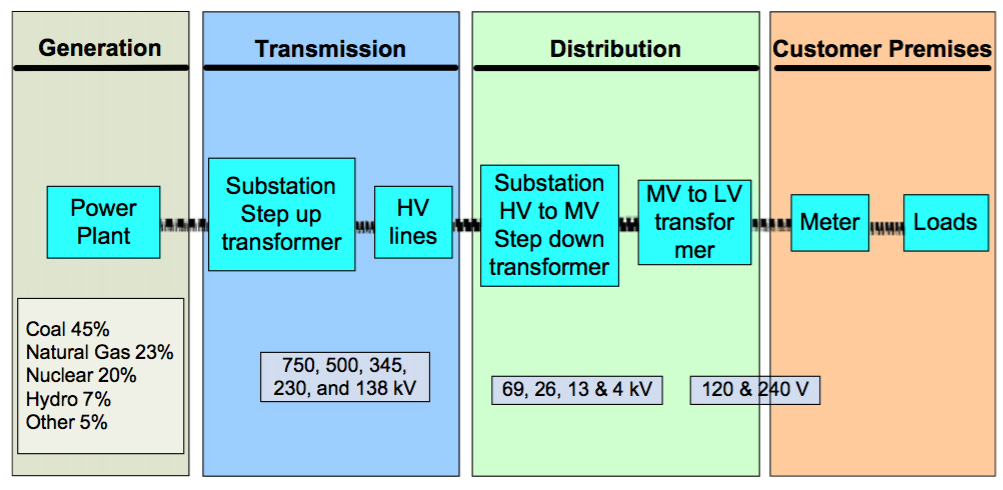
\includegraphics[scale=0.3, natwidth=1003,natheight=490]{imgs/elect_grid.png}}
\caption{La rete elettrica attuale}
\end{figure}
\newline La struttura della rete attuale è una struttura strettamente gerarchica. La figura 1.1 mostra l'esistenza di tre sottosistemi distinti: generazione, trasmissione e distribuzione. \newline Le centrali elettriche sono composte da generatori elettromeccanici i quali, durante la fase di \textbf{generazione}, spinti dal flusso dell'acqua corrente o da motori termici alimentati da combustioni chimiche, generano energia. Tale energia viene successivamente inviata ai trasformatori del livello di \textbf{trasmissione}, i quali la convertiranno in energia ad alto voltaggio per permetterne la diffusione a lunga distanza. Dopo tale step, si passa alla \textbf{distribuzione}, in cui si applica prima una trasformazione a medio e basso voltaggio e, in seguito, si procede all'erogazione agli utenti finali.
\newline Tale sistema è basato sostanzialmente su una comunicazione \textit{unidirezionale} in cui la sorgente non ha nessuna informazione real-time circa le necessità degli ultimi punti della catena. Pertanto si tende a sovraccaricare la rete, facendole raggiungere a priori i picchi massimi di carico; poiché è raro che le richieste degli utenti raggiungano tali valori, questo approccio porta a rendere la rete elettrica un meccanismo inefficiente.
\newline
Inoltre, le reti elettriche attuali sono interconnesse tra loro a formare reti regionali o nazionali con lo scopo di fornire rotte ridondanti e alternative per il flusso della corrente in caso di problemi. \newline
La distribuzione dell'energia è gestita da un \textit{controllore centralizzato} che ha il compito di amministrare diverse regioni da un'unica posizione centrale. 
\newpage
\section{Cenni storici}
Le tecnologie relative alle reti elettriche hanno radici che risalgono alla fine del XIX secolo: la \textit{corrente continua} di Thomas Edison e la \textit{corrente alternata} di Nikola Tesla continuano ad essere utilizzate tutt'ora. Oggi, infatti, l'energia viene trasmessa utilizzando la corrente alternata, mentre quella continua ha applicazioni specifiche, solitamente all'interno di plessi residenziali e commerciali. \newline \newline
Le principali topologie di rete elettrica attualmente in uso sono due: \textbf{radial grid} e \textbf{mesh grid}.


\begin{figure}[h]\centering{
  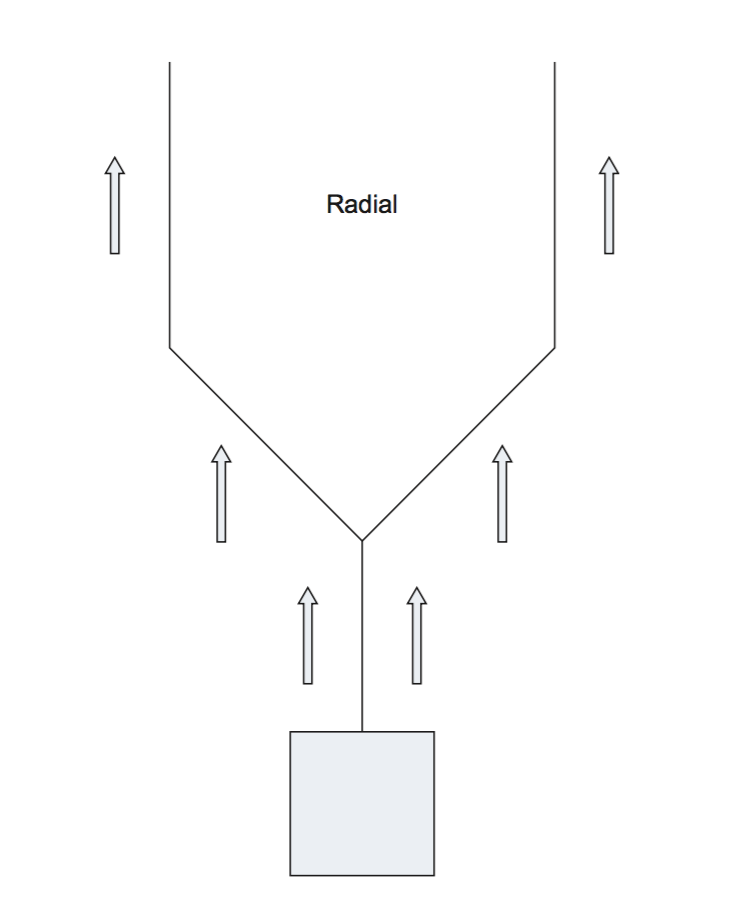
\includegraphics[scale=0.2, natwidth=754,natheight=909]{imgs/radialgrid.png}
  \caption{Radial grid}
}
\end{figure}

La radial grid (figura 1.2) è la topologia più comune; in essa l'elettricità viene distribuita a partire da una sottostazione seguendo un modello che ricorda un albero con molti rami e foglie.
Man mano che l'energia fluisce attraverso i cavi elettrici, la sua forza viene ridotta finchè non raggiunge la destinazione.

\begin{figure}[h]\centering{
  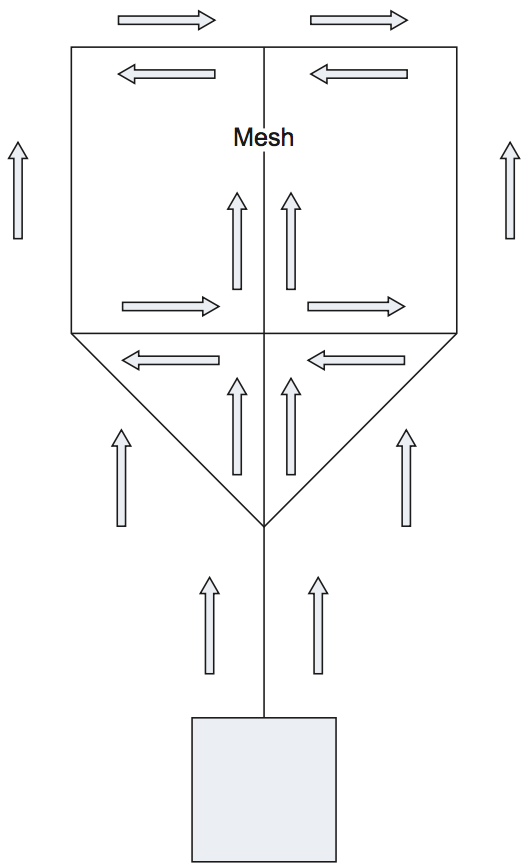
\includegraphics[scale=0.2, natwidth=529,natheight=867]{imgs/meshgrid.png}
  \caption{Mesh grid}
}
\end{figure}

La mesh grid (figura 1.3) fornisce una maggiore affidabilità rispetto alla radial grid poichè in quest'ultima ogni ramo ed ogni foglia ricevono energia da una singola sorgente (l'albero), mentre in una mesh l'energia può essere fornita attraverso varie fonti (altri rami e foglie). \newline
Le radial grid forniscono, inoltre, ridondanza limitata: in caso di malfunzionamento, una sottostazione vicina può entrare a far parte della rete, ma ciò presuppone che tale sottostazione non sia nelle stesse condizioni di quella che ha generato il guasto. \newline
Queste due topologie sono molto diffuse negli Stati Uniti.
Vi è, poi, una terza topologia utilizzata principalmente in Europa: \textbf{looped topology}, nata come insieme delle due reti precedenti (figura 1.4). 

\begin{figure}[h]\centering{
  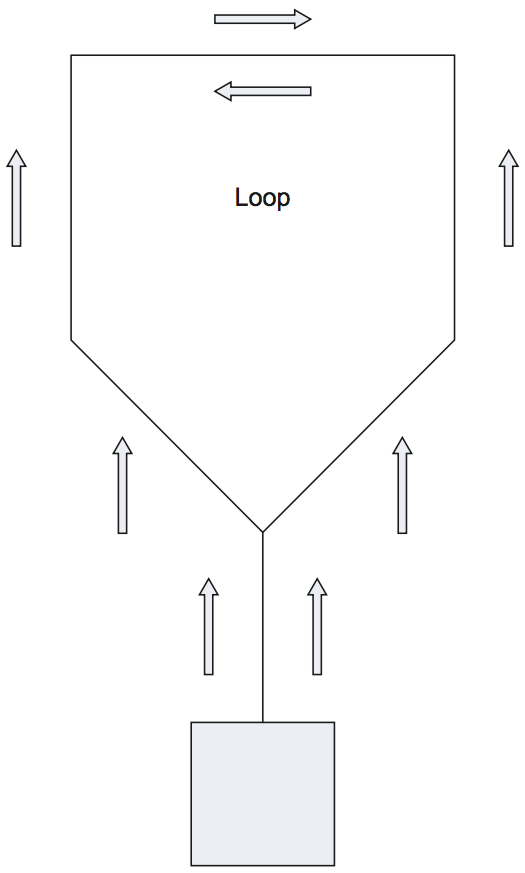
\includegraphics[scale=0.2, natwidth=525,natheight=873]{imgs/looptop.png}
  \caption{Looped topology}
}
\end{figure}
\newpage
Tale topologia è molto simile alla radial grid, ad eccezione del fatto che, a partire dalla sottostazione, i rami e le foglie hanno due cammini separati. L'obiettivo della looped topology è essere capace di resistere alle rotture interne alla rete, indipendentemente dal punto in cui si verificano; per questo motivo tale topologia risulta essere più costosa rispetto alla radial grid.
\newline \newline
Con il passare del tempo si è sentita sempre di più la necessità di svecchiare tali topologie, tenendo in conto tanti fattori e tante motivazioni.\newline
Considerando, per esempio, che quasi il 90\% dei guasti alla rete elettrica provengono dal sottosistema di distribuzione, le modifiche e i miglioramenti partono proprio da quest'ultimo. Inoltre, il rapido aumento dei costi relativi ai combustibili fossili insieme all'inabilità delle aziende di espandere la loro potenza di generazione mantenendola in linea con la domanda sempre più crescente, ha accelerato il bisogno di modernizzare la rete di distribuzione introducendo tecnologie capaci di gestire meglio sia le richieste che i guadagni ottenuti. \newline
\begin{figure}[h]\centering{
  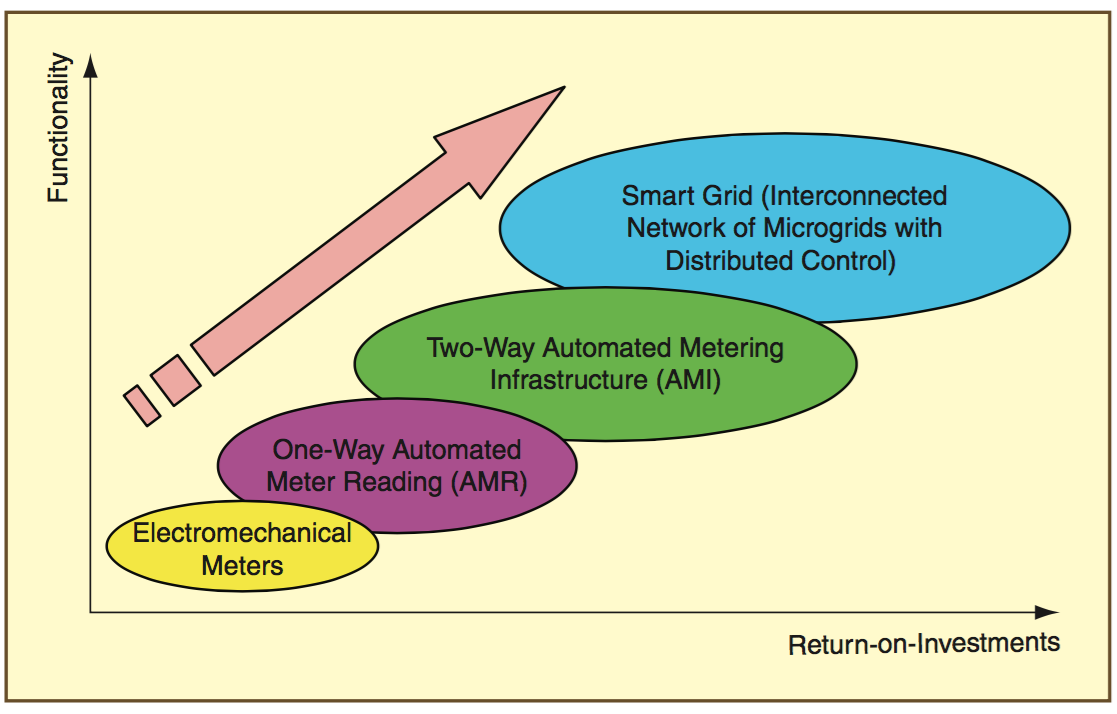
\includegraphics[scale=0.2, natwidth=1117,natheight=714]{imgs/evolution.png}
  \caption{L'evoluzione della smart grid}
}
\end{figure}

La figura 1.5 mostra che gli investimenti degli ultimi anni si sono focalizzati principalmente sull'aspetto della rete elettrica che riguarda le misurazioni (\textit{metering}). \newline I primi progetti in questo settore hanno visto la nascita dei sistemi di \textbf{automated meter reading} (AMR) all'interno del sistema di distribuzione. \newline
L'infrastruttura AMR, nata nel 1977, ha introdotto l'automazione nella rete elettrica. Attraverso una combinazione di tecnologie, incluse reti wireless e wired,   AMR ha permesso alle compagnie di leggere le misurazioni da remoto, di ottenere le informazioni quasi in real-time e di fornire agli utenti bollette basate sui loro consumi reali (in precedenza le compagnie emettevano le bollette basandosi sulle stime dei consumi del cliente).  \newline Inoltre, grazie a questo meccanismo di recupero informazioni tempestivo, le aziende sono state capaci di migliorare la produzione di energia attraverso un maggiore controllo durante periodi di alta e bassa richiesta. \newline \newline
Sebbene la teconologia AMR all'inizio abbia attirato molta attenzione, le aziende presto si sono rese conto che non risolve il loro problema principale: la gestione demand-side. A causa della sua comunicazione unidirezionale, le capacità di AMR sono ridotte alla sola lettura dei dati e non è permesso, per esempio, modificare il comportamento della rete a seconda delle informazioni ricevute. \newline Pertanto AMR ha avuto vita breve; le aziende, piuttosto che continuare ad investire su di essa, hanno preferito spostarsi verso l'\textbf{advanced metering infrastructure} (AMI). \newline
L'AMI (di cui si parlerà in dettaglio nel capitolo 2), è un'architettura che permette la comunicazione automatizzata e bidirezionale tra uno smart meter e una società di servizi. L'obiettivo è quello di fornire a tali società informazioni real-time circa i consumi energetici e permettere agli utenti di fare scelte consapevoli sull'utilizzo dell'energia basate sui costi all'istante di utilizzo.
\newline
\newline
Il passo successivo nell'evoluzione della distribuzione della corrente elettrica è costituito dalla \textbf{Smart Grid}, che utilizza l'AMI come componente core per il recupero delle informazioni circa lo stato della rete e i consumi utente.
\newpage

\section{Perché la Smart Grid?}
Le industrie del settore dei servizi pubblici di tutto il mondo attualmente cercano di risolvere numerosi problemi, tra cui 
\begin{itemize}
\item diversificazione della generazione di energia
\item gestione delle richieste utente
\item conservazione dell'energia
\item riduzione globale dell'emissione di anidride carbonica
\end{itemize}
È evidente che tali problemi non possono essere risolti facendo affidamento sulla rete elettrica esistente. \newline
Come detto in precedenza, la natura della comunicazione della rete attuale è unidirezionale. Essa, inoltre, converte solo un terzo di energia in elettricità, senza preoccuparsi del calore disperso. Circa l'8\% della corrente prodotta, viene dissipata poi attraverso i cavi elettrici, mentre il 20\% viene riservata ad eventuali picchi di carico di richieste utente (ed è in uso solo il 5\% delle volte). \newline
In aggiunta a tali problemi, vi è l'inadeguatezza della struttura gerarchica della rete. A causa di tale organizzazione, infatti, si ha un \textit{effetto domino dei guasti}, in cui un fallimento verificatosi all'interno di uno dei tre sottosistemi può influire significativamente sugli altri. \newline
La rete elettrica di nuova generazione, la Smart Grid, si propone di occuparsi delle maggiori carenze della rete attuale.
\begin{figure}[h]\centering{
  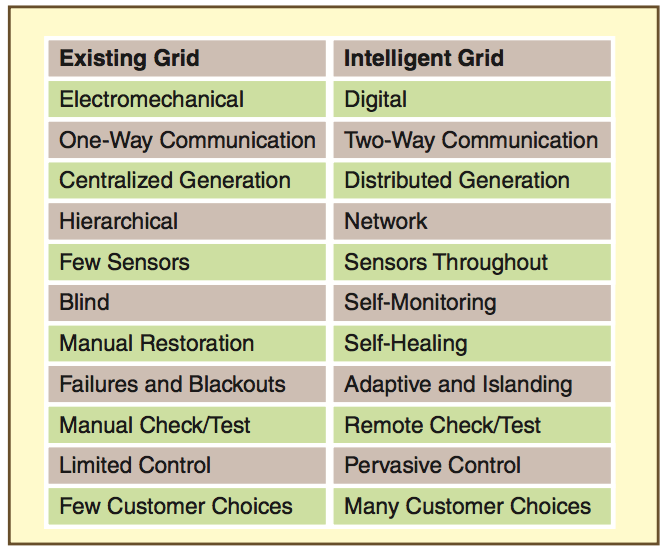
\includegraphics[scale=0.3, natwidth=669,natheight=553]{imgs/differences.png}
  \caption{Differenze tra la rete elettrica attuale e la Smart Grid}
}
\end{figure}

A partire dal 2005, c'è stato un interesse sempre più crescente verso le Smart Grid. Il riconoscere che l'ICT (\textit{Information and Communication Technology}) offre significative opportunità per modernizzare il funzionamento delle reti elettriche unito alla consapevolezza che la produzione di energia può essere migliorata solo con un continuo ed efficiente monitoraggio, ha fatto sì che si muovessero i primi passi verso la Smart Grid. In aggiunta a tali fattori, ci sono anche altre motivazioni a favore del passaggio verso una rete elettrica moderna:
\begin{itemize}
\item \textit{Strutture non più adeguate}: in molte zone del mondo (per esempio in USA e in alcuni paesi dell'Europa), i sistemi si sono rapidamente espansi a partire dal 1950; le strutture relative alla trasmissione e alla distribuzione che furono installate a quel tempo non sono più adatte e hanno bisogno di essere sostituite. \newline Il bisogno di rinnovare tali componenti è un'ovvia opportunità di innovazione e, quindi, di introduzione di nuovi modelli e pratiche operative. \newline A ciò si aggiunge il fatto che, in molti paesi, i circuiti elettrici hanno bisogno di adattarsi ai carichi sempre più crescenti e all'introduzione di nuove fonti di energia rinnovabili. Ciò richiede, quindi, metodi più intelligenti sia per aumentare la capacità di trasmissione dell'energia, sia per reindirizzare il flusso di corrente verso circuiti meno carichi.

\item \textit{Vincoli termici}: tali vincoli si riferiscono ai limiti dei sistemi di trasmissione e distribuzione relativamente alla loro capacità di diffusione dell'energia. Quando le attrezzature trasportano la corrente eccedendo la loro potenza termica, si surriscaldano e i materiali atti all'isolamento si deteriorano rapidamente. Ciò comporta una riduzione della vita delle attrezzature e un aumento di possibilità dei fallimenti.\newline I vincoli termici dipendono molto dalle condizioni dell'ambiente esterno, che cambiano durante gli anni. Pertanto l'uso di rate di trasmissione e distribuzione dinamici può aumentare la capacità del circuito in qualsiasi momento.

\item \textit{Vincoli operativi}: qualsiasi sistema opera all'interno di predefiniti vincoli di voltaggio e frequenza. Se il voltaggio eccede il limite, i materiali isolanti dei componenti del sistema e le attrezzature degli utenti possono essere danneggiate e causare corto-circuito. \newline Per quanto riguarda la frequenza invece, si tende a mantenerla all'interno di un range molto piccolo e, quando varia, intervengono dei servizi appositi che hanno il compito di riportarla nell'intervallo prestabilito. \newline
La generazione di energia rinnovabile, però, ha un output variabile che non può essere previsto con certezza in anticipo. Pertanto mantenere il bilancio erogazione-richiesta e la frequenza del sistema nei limiti risulta essere un compito arduo. Per tale motivo si è sempre alla ricerca di nuovi servizi per la gestione della frequenza. \newline Si pensa che in futuro l'utilizzo delle Smart Grid in vari ambiti, per esempio domestico e automobilistico, porterà ad avere carichi sempre più flessibili; ciò aiuterà nel mantenere la stabilità della rete.

\item \textit{Sicurezza delle forniture}: la società moderna richiede che la fornitura di energia sia sempre più affidabile, man mano che carichi sempre più critici vengono connessi alla rete. L'approccio tradizionale per migliorare l'affidabilità, come visto in precedenza, era quello di installare cammini ridondanti, con notevole impatto sia sui costi che sull'ambiente. \newline L'approccio della Smart Grid in caso di guasti, invece, prevede l'utilizzo di intelligenti meccanismi di riconfigurazione, in modo tale da mantenere costante la fornitura ai clienti ma evitando i costi addizionali portati da ulteriori circuiti.
\item \textit{Iniziative nazionali}: molti governi nazionali incoraggiano le iniziative delle Smart Grid poiché le considerano un meccanismo redditizio ma, allo stesso tempo, economico per rinnovare le loro infrastrutture e introdurre risorse rinnovabili.
\end{itemize}

\begin{figure}[h]\centering{
  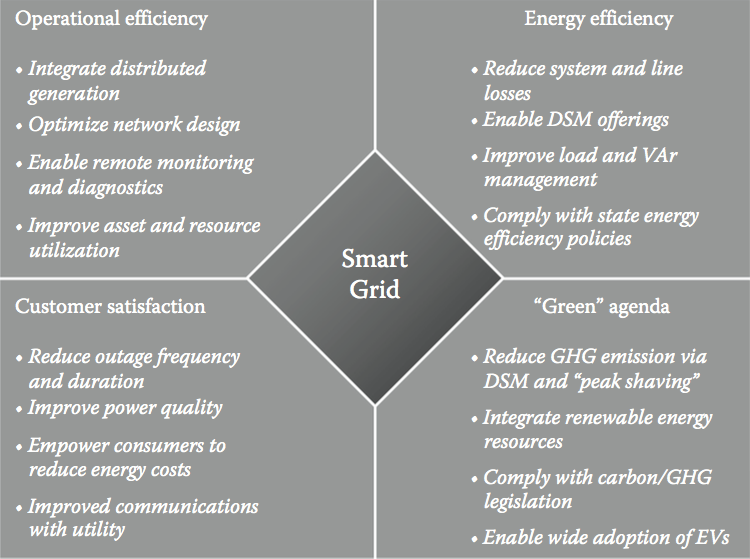
\includegraphics[scale=0.3, natwidth=750,natheight=559]{imgs/benefits.png}
  \caption{Benefici introdotti dalla Smart Grid}
}
\end{figure}

La figura 1.7 mostra i vantaggi introdotti dall'utilizzo delle Smart Grid. Lo sviluppo di tale rete moderna non dovrebbe essere basato solo su ``soluzioni abilitanti", ma anche su ``soluzioni integrate" che rispondano ai problemi operativi e aziendali e che forniscano benefici significativi, misurabili e durevoli agli utenti, al servizio pubblico, all'economia e all'ambiente.
\newline 
Di estrema importanza nell'implementazione delle soluzioni proposte dalla Smart Grid sono i seguenti risultati:
\begin{itemize}
\item migliorare l'affidabilità dell'energia dei servizi pubblici, le performance operative e la produttività generale
\item aumentare l'efficienza energetica e diminuire le emissioni di anidride carbonica
\item permettere agli utenti di gestire i loro consumi energetici risparmiando energia ma, allo stesso tempo, senza modificare il loro stile di vita
\item ottimizzare l'integrazione di energie rinnovabili 
\end{itemize}

\section{Cos'è la Smart Grid?}
Il concetto di Smart Grid mette insieme una serie di tecnologie e soluzioni per gli utenti finali e affronta, inoltre, concetti politici e normativi. \newline Non esiste una singola definizione chiara e precisa; l'European Technology Platform [ref] definisce la Smart Grid nel seguente modo:
\begin{quote}
\textit{``Una Smart Grid è una rete elettrica che può integrare intelligentemente le azioni di tutti gli utenti connesse ad essa - generatori, consumatori - in modo da fornire efficientemente un'alimentazione elettrica che sia sostenibile, economica e sicura."}
\end{quote}
In accordo all'US Department of Energy [ref]:
\begin{quote}
\textit{``Una Smart Grid utilizza la tecnologia digitale per migliorare l'affidabilità, la sicurezza e l'efficienza (sia economica che energetica) del sistema elettrico, ...RIVEDERE TRADUZIONE ... "}
\end{quote}
[4 ref] suggeriscono i seguenti attributi per una Smart Grid:
\begin{itemize}
\item Permette la gestione ``demand side" sia attraverso l'integrazione di smart meter, elettrodomestici intelligenti, micro-generazione e conservazione dell'energia sia fornendo agli utenti informazioni circa i loro utilizzi e i prezzi
\item Facilita l'introduzione di fonti di energia rinnovabile e di generazione distribuita, riducendo così l'impatto ambientale dell'intero settore energetico 
\item Assicura e migliora l'affidabilità e la sicurezza delle forniture, resistendo agli attacchi, ai disturbi e ai disastri naturali, anticipando e affrontando i problemi del sistema e migliorando le funzionalità di trasferimento dell'energia
\item Mantiene alta la qualità della fornitura di energia elettrica per soddisfare le apparecchiature sempre più sofisticate che aumentano con l'economia digitale
\end{itemize}
\begin{figure}[h]\centering{
  
\includegraphics[scale=0.25, natwidth=1522,natheight=466]{imgs/wordcloud.png}
}
\end{figure}
\section{Requisiti di una Smart Grid}
Monitoraggio/sensing, comunicazione e controllo sono i tre building block fondamentali che convertono un sistema di distribuzione di energia in una Smart Grid. Le componenti di monitoraggio/sensing devono essere capaci di rilevare malfunzionamenti o deviazioni dal normale range operativo della rete elettrica. Inoltre, poiché in una Smart Grid un punto di consumo elettrico può diventare anche un punto di generazione, il processo di sensing deve essere strettamente collegato al processo di metering. \newline
I sistemi di comunicazione devono permettere che l'input dei sensori raggiunga gli elementi di controllo della Smart Grid, i quali genereranno dei messaggi con il compito di assicurarsi che la trasmissione nei vari punti della rete sia conforme alle aspettative. Ci sono, inoltre, altri requisiti importanti per le infrastrutture di comunicazione, di cui si discutono i dettagli nel resto di questo paragrafo.
\newline \newline
\textit{Quality of Service:} è necessario garantire la QoS per le tecnologie di comunicazione e di rete utilizzate all'interno della Smart Grid, partendo dalla generazione dell'energia, passando per trasmissione e distribuzione e finendo alle applicazioni utente. In particolare, ci si focalizza su due parametri: latenza e larghezza di banda.\newline
Per quanto riguarda la latenza, la comunicazione in una Smart Grid è caratterizzata dal fatto che la maggior parte delle interazioni devono avvenire in tempo reale. Per scopi di sensing/misurazione, i messaggi di lettura dovrebbero essere trasmessi all'interno di un frame temporale molto piccolo. Per esempio, il tempo massimo di trasmissione ammesso è nel range dei 12-20 ms. I valori misurati non dovrebbero essere generati da più di 15 secondi quando arrivano al centro di controllo. \newline
Per quanto riguarda la larghezza di banda, mano mano che la Smart Grid evolve e, quindi, si aggiungono ad essa elementi sempre più intelligenti, l'infrastruttura di comunicazione dovrebbe essere capace di trasmettere un numero sempre più crescente di messaggi simultaneamente, senza grave impatto sulla latenza. La banda di rete deve aumentare più rapidamente rispetto alla richiesta di tali elementi intelligenti nella rete.
\newline \newline
\textit{Interoperabilità:} si riferisce all'abilità delle diverse parti di una Smart Grid di lavorare insieme, di utilizzare componenti compatibili, di scambiarsi informazioni tra di loro e lavorare in maniera cooperativa per completare i task. Tale requisito rende effettiva l'integrazione e la comunicazione bidirezionale tra i tanti elementi interconnessi della rete.\newline
Il NIST ha sviluppato un framework che include protocolli e standard per la gestione delle informazioni, in modo da raggiungere l'interoperabilità tra i dispositivi della Smart Grid e i sistemi. Maggiori dettagli in [ref].
\newline \newline
\textit{Scalabilità:} è necessaria per facilitare l'inserimento all'interno della Smart Grid sia di tanti nuovi dispositivi e servizi, che di tanti meccanismi di monitoraggio real-time dell'interazione dell'utente finale. \newline
[ref] propone una rete IP-based come soluzione efficace per i bisogni dell'infrastruttura di comunicazione.
\newline \newline
\textit{Sicurezza:} in accordo all'Electric Power Research Institute (EPRI), uno dei requisiti emergenti dello sviluppo delle Smart Grid è relato alla cyber security dei sistemi. Come indicato nel loro report [ref], la sicurezza informatica del sistema di comunicazione è un problema critico, a causa dell'aumento del potenziale degli attacchi e degli incidenti che si verificano in esso. \newline 
La cyber security deve occuparsi non solo di attacchi deliberati, come quelli provenienti, ad esempio, da dipendenti non contenti, da spionaggio industriale e da terroristi, ma anche di manomissioni involontarie dell'infrastruttura di informazione dovute ad errori degli utenti, fallimenti delle attrezzature e disastri naturali. Le vulnerabilità potrebbero permettere, infatti, ad un attaccante di penetrare nella rete, ottenere accesso al software di controllo e alterare le condizioni di carico per destabilizzare la rete. \newline
Attualmente, molte organizzazioni lavorano sullo sviluppo dei requisiti di sicurezza nella Smart Grid, tra cui North American Electrical Reliability Corporation-Critical Infrastructure Protection (NERC-CIP), IEEE, National Infrastructure Protection Plan (NIPP), e NIST. \newline 
Denominatore comune di tutti gli standard in via di sviluppo è il seguente concetto: la sicurezza delle comunicazioni nella Smart Grid dipenderà fortemente da autenticazione, autorizzazione e tecnologie per la privacy. \newline Tutte le teconologie sviluppate, poggiano su una sorta di gestione della chiave. Considerando il fatto che la Smart Grid conterrà milioni di dispositivi, diffusi tra tante organizzazioni, i sistemi di gestione della chiave utilizzati dovranno essere scalabili a livelli straordinari e dovranno garantire, inoltre, i livelli massimi possibili di efficienza[ref].
\newline \newline
\textit{Standardizzazione:} la Smart Grid coinvolge al suo interno una serie di standard come, ad esempio, nella generazione dell'energia, nella distribuzione e nel controllo oltre che nella comunicazione. IEEE recentemente ha preso l'iniziativa per definire questi standard e per scrivere delle linee guida su come la Smart Grid dovrebbe operare utilizzando le ultime tecnologie nell'ingegnerizzazione dell'energia, controllo, comunicazione e informazione; il gruppo che è stato creato prende il nome di IEEE P2030 group [ref]. \newline Per quanto riguarda l'ingegnerizzazione dell'energia, ci si focalizza sui requisiti di interoperabilità. Per quanto riguarda l'informazione, invece, si affrontano problemi relativi alla privacy, sicurezza, integrità dei dati, interoperabilità e interfacce. Per la comunicazione, infine, si definiscono i requisiti per l'interazione tra i dispositivi e si stabiliscono limiti per generazione, distribuzione e trasmissione in collaborazione con i clienti.
 
\newpage
\section{Tecnologie coinvolte}
Per soddisfare tutti i requisiti della Smart Grid, è necessario sviluppare ed implementare le seguenti tecnologie:
\begin{enumerate}
\item \textit{Tecnologie per l'informazione e la comunicazione}, che includono
	\begin{itemize}
	\item meccanismi per la comunicazione bidirezionale tra le varie componenti del sistema
	\item architetture aperte per il collegamento e l'utilizzo semplice di elettrodomestici e veicoli elettrici
	\item componenti hardware e software necessari per fornire ai clienti sempre più informazioni
	\item software per garantire la sicurezza delle informazioni e standard per fornire scalabilità e interoperabilità tra i sistemi di informazione e comunicazione
	\end{itemize} 
\item \textit{Tecnologie per misurazioni, sensing, controllo ed automazione}, che includono
	\begin{itemize}
	\item \textit{Intelligent Electronic Devices} (IED) per fornire inoltro, misurazioni e memorizzazione di fallimenti ed eventi per il sistema energetico in maniera avanzata
	\item \textit{Phasor Measurement Units} (PMU) e \textit{Wide Area Monitoring, Protection and Control} (WAMPAC) per garantire la sicurezza del sistema
	\item sistemi integrati di sensing, misurazione, controllo ed automazione e tecnologie per l'informazione e la comunicazione per fornire rapide diagnosi e risposte tempestive a qualsiasi evento in qualsiasi parte della rete
	\item elettrodomestici, comunicazione, controllo e monitoraggio più intelligenti per massimizzare la sicurezza, il comfort e il risparmio energetico delle abitazioni
	\item smart meter e tutti i software che permettano ai clienti di avere una maggiore scelta e un maggiore controllo sull'utilizzo di elettricità e gas. \newline Tali meccanismi permetteranno, inoltre, di fornire ai clienti bollette più accurate e informazioni real-time più precise sui loro consumi
	\end{itemize}
\item \textit{Tecnologie per la conservazione dell'energia}, che includono
	\begin{itemize}
	\item \textit{High Voltage Direct Current} (HVDC) e \textit{Flexible Alternate Current Transmission Systems} (FACTS) per abilitare le trasmissioni a lungo raggio e l'integrazione delle energie rinnovabili
	\item differenti interfacce e differenti dispositivi per fornire una connessione efficiente delle risorse rinnovabili e dei dispositivi per la conservazione dell'energia
	\item dispositivi per fornire un maggiore controllo sui flussi di energia nella rete a corrente alternata
	\item  HDVC e FACTS in unione ad altri filtri, integrati nei meccanismi di comunicazione e controllo per assicurare una maggiore affidabilità e flessibilità del sistema e una migliore qualità dell'energia
	\end{itemize}
\end{enumerate}
\chapter{Architettura}
L'odierna rete elettrica è stata progettata come un sistema centralizzato, in cui l'energia elettrica fluisce attraverso linee unidirezionali di trasmissione e distribuzione dai generatori fino ai clienti finali. La logica applicativa è concentrata in zona centrale e solo parzialmente nelle \emph{substation}, mentre le componenti restanti sono quasi totalmente passive. Una Smart Grid, mostrata dal punto di vista strutturale in figura \ref{fig:21}, fornisce una più elevata ed ampia intelligenza distribuita incorporata nei dispositivi locali, comunicazione e scambio bidirezionale di informazioni ed elettricità.

\begin{figure}[h] \centering{
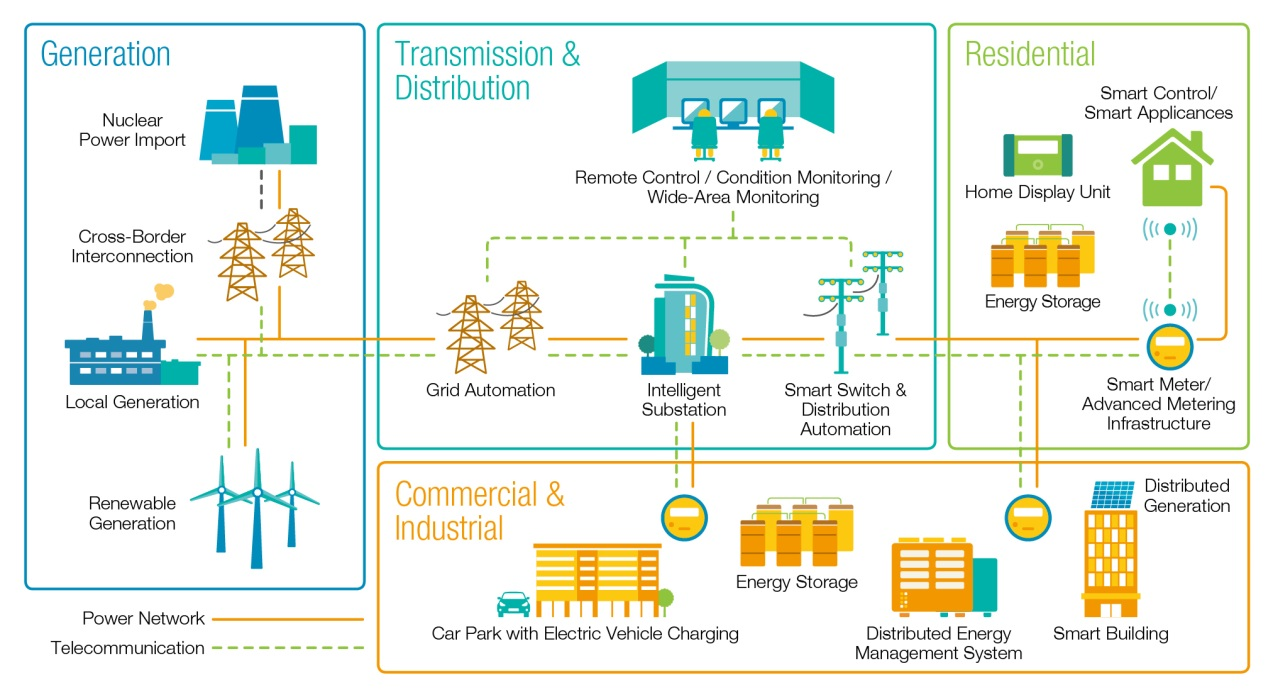
\includegraphics[scale=0.95]{imgs/architecture.jpg}}
\caption{Smart Grid}\label{fig:2_1}
\end{figure}

\section{Smart Grid Framework}
Le Smart Grid richiedono sia una complessa infrastruttura di comunicazione, che sofisticate tecnologie di comunicazione e computazione. Entrambe consentono la conservazione di parte dell'energia prodotta e l'introduzione di nuovi metodi di gestione della domanda energetica, per adottare politiche di bilanciamento del carico, controllare instabilità energetiche causate dalla natura delle risorse rinnovabili e prevenire la diffusione di fallimenti in cascata nella rete. 
\\ 
La figura \ref{fig:22} riassume le principali tematiche relative alle Smart Grid:
\begin{itemize}
	\item \emph{Energy infrastructure} rappresenta la base fisica ed organizzativa necessaria per la generazione, trasmissione e distribuzione dell'energia;
	\item \emph{Communication infrastructure} è responsabile del trasferimento di informazioni critiche attraverso la rete;
	\item \emph{Information technology} fornisce modelli, analisi, visualizzazioni web e transazioni commerciali;
	\item \emph{Potential applications} offre tecniche di generazione, gestione, automatizzazione e rilevamento per l'intero sistema.
\end{itemize} 

\begin{figure}[h] \centering{
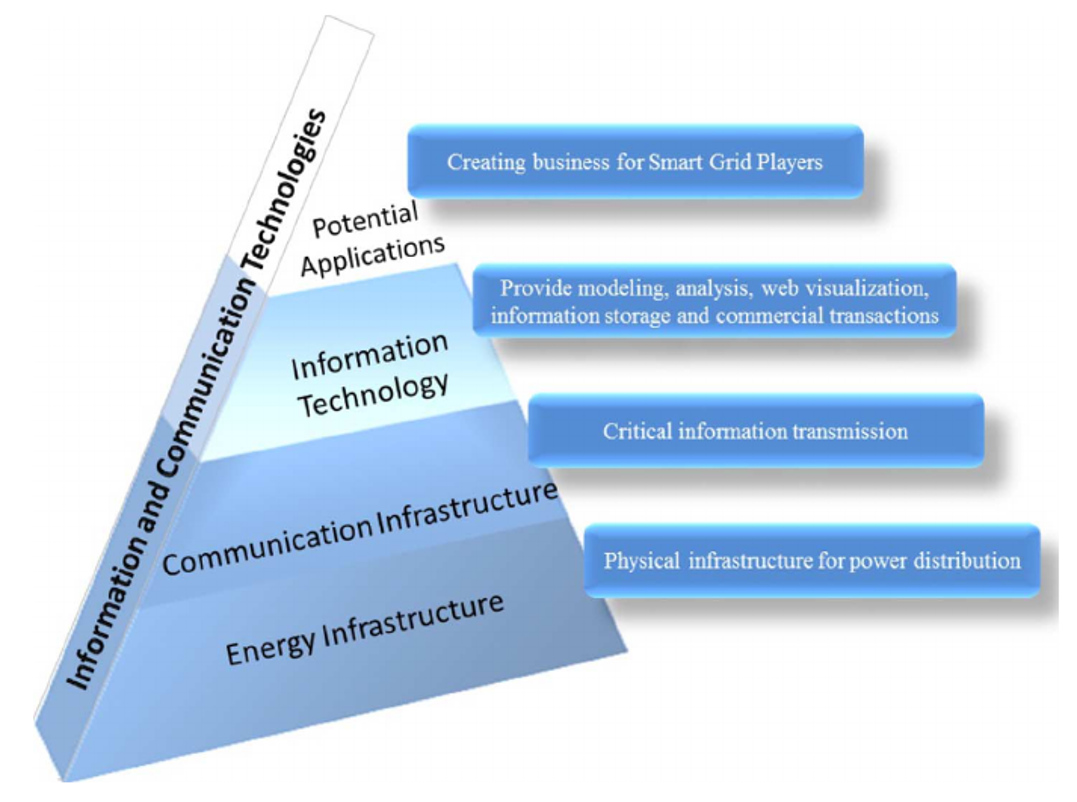
\includegraphics[scale=0.3, natwidth=1003,natheight=490]{imgs/ict.png}}
\caption{Smart Grid framework}\label{fig:22}
\end{figure}

La communication infrastructure svolge un ruolo cruciale, ossia collegare tutte le componenti della rete collezionando informazioni sulle loro condizioni, per scopi di controllo, monitoraggio e manutenzione. Eventuali problemi legati all'energy instrastructure possono essere evitati se corrette operazioni vengono prese con l'aiuto della communication infrastructure. 
\\ 
Differenti tecnologie di comunicazione posso essere usate per diversi scopi e requisiti in base all'applicazione. L'information technology fornisce una piattaforma comune di scambio di informazioni proveniente da differenti attività legate alla Smart Grid, che permette l'integrazione di informazioni da diversi livelli, dando sostegno alla raccolta di diverse informazioni, all'analisi e ad applicazioni avanzate.
\\
Le tecniche dell'applications layer generalmente mirano a ridurre il consumo energetico dei clienti, cambiando i loro comportamenti di consumo, dotandoli di strumenti di monitoraggio.    
\\
La figura \ref{fig:23} mostra le componenti della Smart Grid, illustrate dall'energy infrastructure al potentional applications.

\begin{figure}[h] \centering{
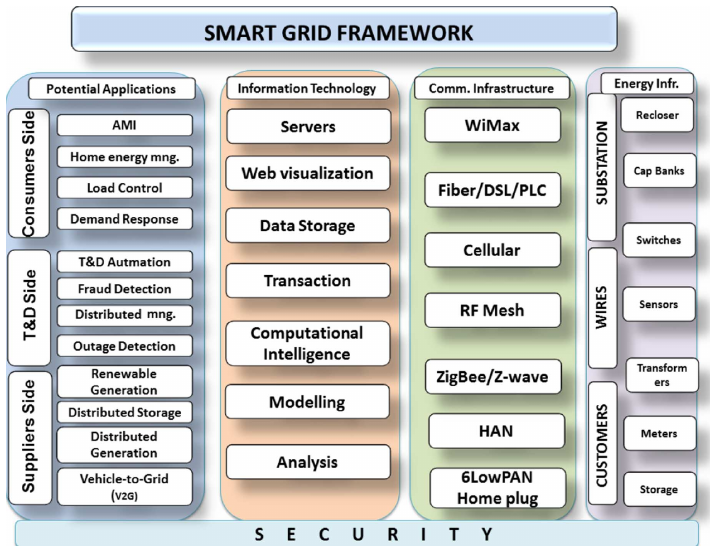
\includegraphics[scale=0.7, natwidth=1003,natheight=490]{imgs/sgframework.png}}
\caption{Smart Grid framework}\label{fig:23}
\end{figure}

%\section{Communication architecture}
\newpage
Il concetto di Smart Grid mira a realizzare un sofisticato sistema, integrando information technology e communication infrastructure all'attuale sistema di alimentazione e il nuovo sistema di generazione distribuito, in modo da sfruttare pienamente l'uso di risorse rinnovabili e di massimizzare l'efficienza energetica. Da una prospettiva leggermente diversa, una Smart Grid può essere considerata come una rete di comunicazione di dati che riesce, grazie al supporto di specifici dispositivi di gestione dell'energia, a far collaborare le diverse componenti della rete in maniera flessibile e senza discontinuità, per un utilizzo efficiente dell'energia.
%\\
%L'architettura \emph{end-to-end} delle Smart Grid (figura \ref{fig:4}) fondamentalmente comprendono tre livelli principali:
%\begin{itemize}
%	\item \emph{Application layer}, include applicazioni avanzate fornendo interoperabilità fra di esse; si occupa principalmente della gestione della domanda/risposta, interruzioni, infrastruttura di metering, delle risose ed rilevamento di frodi;
%	\item \emph{Power layer}, comprende i sistemi di generazione, trasmissione e distribuzione, l'integrazione di risorse rinnovabili ed il sistema di comunicazione bidirezionale;  
%	\item \emph{Communication layer}, rappresenta il cuore del sistema fornendo la connettività fra tutte le parti e dispositivi di esso. 
%\end{itemize}     

%\begin{figure}[h] \centering{
%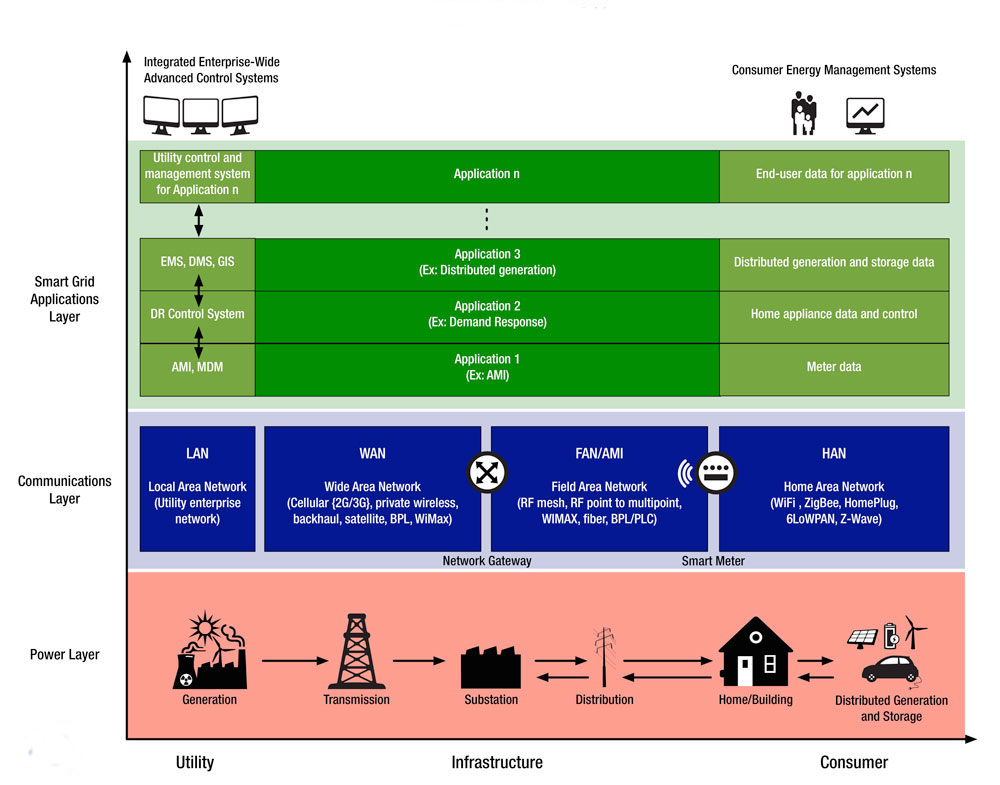
\includegraphics[scale=0.4, natwidth=1003,natheight=490]{imgs/endtoendtax.jpg}}
%\caption{Architettura end-to-end}\label{fig:4}
%\end{figure}

La comunicazione consiste di tre categorie di trasmissione, con relativi standard e protocolli (vedi capitolo):
\begin{itemize}
	\item \emph{Wide-area network} (WAN);
	\item \emph{Field-area network} (FAN);
	\item \emph{Home-area network} (HAN).
\end{itemize}

\subsection{Wide-area network}
La WAN consente la comunicazione fra le entità che forniscono energia e le substations; deve estendersi su tutte le substation, strutture di distribuzione, generazione energetica e di conservazione dell'energia, per poter essere efficace e scalabile. Essa è rete di comunicazione bidirezionale ad alta larghezza di banda che gestisce le trasmissioni a lunga distanza dei dati con avanzate applicazioni di misurazione e monitoraggio. La comunicazione remota fra le \emph{utility} e gli smart meter è essenziale per lo scambio di importanti informazioni, quali prezzi e tariffe dei clienti. Le reti cellulari, WiMAX e comunicazioni cablate, in particolare comunicazioni basate su fibra ottica e microwave, sono i migliori candidati come tecnlogie per WAN (vedi capitolo 4).
\\
Il sistema di distribuzione agisce da punto di aggregazione fra FAN e WAN, come ad esempio una substation o una torre di comunicazione che colleziona tutte le informazioni prodotte dagli smart meter e le trasferisce alla rete di comunicazione principale. Oltre che da punto di aggregazione tali dispositivi possono fungere da punti di conservazione dell'energia per eventuali interruzioni o guasti.

\subsection{Field-area network}
La FAN può essere descritta come una rete di comunicazione per aree di distribuzione dell'energia e che mette in contatto l'automazione della distribuzione e dispositivi di controllo alle sedi dei consumatori. Essa agisce, quindi, come un intermediario fra le substation e le sedi dei clienti, con nodi intelligenti in grado di raccogliere e controllare i dati da remoto. Tali nodi sono connessi ad un gateway centralizzato, il quale è alimentato costantemente in modo da poter trasmettere i dati raccolti. I canali a bassa larghezza di banda della FAN sono altamente robusti per la trasmissione affidabile di dati. 
\\ 
La scelta delle tecnologie di comunicazione  variano per la FAN in base alle esigenze della Smart Grid: fibra ottica per avere bassa latenza e perfomance di comunicazione superiori, oppure WiMAX se le reti cellulari non riescono a coprire l'area di interesse, ma l'attuale orientamento ricade sull'utilizzo dello standard IEC 61850 (vedi capitolo ), il quale fornisce interoperabilità e comunicazione fra i dispositivi elettronici intelligenti.

\subsection{Home-area network}{
Gli smart meter riescono a connettersi alla HAN, in modo tale che i consumatori siano in grado di conoscere l'importo da pagare e gestire il loro consumo ed avere il controllo dei propri elettrodomestici intelligenti, attraverso display presenti in casa e interfacce web. 
\\ 
Le migliori tecnologie di comunicazione per HAN sono ZigBee,Wi-Fi, HomePlug, Z-wave e M-Bus (vedi capitolo).
}

\vspace{20pt}\hspace{-17pt}Nelle sezioni successive vengono presentate le tecnologie e le infrastrutture abilitanti di una Smart Grid, a partire dalla generazione e conservazione dell'energia fino ad arrivare alla trasmissione e distribuzione.

\section{Generazione di energia rinnovabile}
Le risorse di energia rinnovabile sono state sviluppate in molti paesi per ridurre l'inquinamento e fornire energia elettrica sostenibile. A differenza delle tradizionali fonti di energia, le quali creano inquinamento, le risorse di energia rinnovabile non esauriscono risorse naturali nel processo di creazione di energia e sono adattabili ovunque, in base alle dimensioni a partire dall'applicazione su una singola casa fino a dimensioni su larga scala.
\\
Le più comuni risorse di energia rinnovabile sono:
\begin{itemize}
	\item \emph{Sistemi fotovoltaici}, i quali convertono l'energia solare direttamente in elettricità, attraverso pannelli solari esposti al sole. Tali pannelli sono costituiti da celle solari che contengono materiale fotovoltaico, le quali trasmettono elettroni tra diverse bande all'interno del materiale generando differenza di potenziale fra due elettrodi, che consente alla corrente continua di fluire;
	\item \emph{Sistemi per l'energia solare termica}, che convertono energia solare in calore. Esistono tre tipi di raccoglitori in base alla temperatura, da bassa per riscaldare piccoli spazi ad alta per l'utilizzo nella produzione di energia elettrica;
	\item \emph{Vento}, la cui energia viene convertita tramite turbine in elettricità. Il principale aspetto negativo deriva dall'intermittenza del vento, specularmente per i sistemi basati sull'energia solare;
	\item \emph{Biomasse}, ovvero la produzione di elettricità a partire da elementi naturali morti, anche se questa causa inquinamento atmosferico;
	\item \emph{Sistemi che sfruttano la potenza dell'acqua}, sia che essa sia generata artificialmente che naturalmente, grazie alle onde e alle maree.   
\end{itemize} 

\section{Smart meter e Advance Metering Infrastructure}
Uno \emph{smart meter} è un dispositivo elettronico che registra consumi di energia elettrica in intervalli di un'ora o meno e comunica tali informazioni per scopi di fatturazione e monitoraggio [7]. Gli smart meter consentono una comunicazione bidirezionale fra essi ed i sistemi di controllo. A differenza dei display energetici posizionati nelle case, gli smart meter possono inviare in remoto i dati raccolti. 
\\
Per quanto riguarda la comunicazione bidirezionale esistono diversi protocolli:
\begin{itemize}
	\item ANSI C12.18, C12.19 e C12.21 , utilizzati principalmente nel nord America;
	\item IEC 61107 e 62056 usati nell'Unione Europea;
	\item  \emph{Open Smart Grid Protocol} (OSGP), famiglia di specifiche pubblicata dall'European Telecommunications Standards Institute, usato in congiunzione con ISO/IEC 14908.
\end{itemize}
Gli smart meter forniscono un modo di misurare informazioni specifiche, che consente alle aziende di introdurre diversi prezzi sul consumo in base al periodo del giorno e alla stagione. Dal punto di vista dei clienti, gli smart meter consentono di conoscere il proprio consumo e regolarsi di conseguenza. Uno studio accademico sulla base di studi esistenti ha mostrato che il consumo di energia elettrica dei proprietari di abitazione, in media, si riduce di circa il 3-5\% [8].
\emph{Advance Metering Infrastructure} è una tecnologia che non coinvolge soltanto gli smart meter, ma è anche un'infrastruttura di comunicazione, applicazioni ed interfacce  per lo scambio di dati. Un tipico sistema AMI (vedi Figura \ref{fig:2_12}) è composto da una centralina AMI per la comunicazione, una piattaforma integrata, un \emph{meter data management system} (MDMS), una rete di comunicazione AMI e terminali AMI, inclusi gli smart meter. I collegamenti di comunicazione con i clienti avviene mediante HAN, attraverso un'interfaccia che comunica con i termostati, elettrodomestici ed altri dispositivi. La centralina monitora, controlla e gestisce i protocolli di comunicazione e lo scambio dei dati con la rete. Inoltre, la centralina permette agli operatori remotamente di monitorare  e gestire la rete AMI. Il MDMS colleziona i dati degli smart meter, effettua conservazione dei dati e li gestisce.
Fra i principali benefici dei sistemi AMI:
\begin{itemize}
	\item Dati preziosi per il rilevamento di interruzioni, che sono intergrati con l'OMS;
	\item Rilevamento e notificazione in caso di manomissioni o furti;
	\item Aspetto chiave per programmi di gestione della domanda energetica;
	\item Maggiori informazioni sui clienti per compagnie;
\end{itemize}

Alcuni svantaggi potenziali dei sistemi AMI:
\begin{itemize}
	\item Problemi di privacy, in quanto le informazioni sull'utilizzo di energia sono disponibili per ciascun cliente e si possono trarre informazioni personali;
	\item Maggiore possibilità di una terza parte non autorizzata di poter accedere ai dati;
	\item Aumento dei rischi per la sicurezza di rete o l'accesso remoto.
\end{itemize}
 
\section{Conservazione dell'energia}
Il principale problema con l'energia elettrica è che deve essere utilizzata non appena viene generata, o in caso contrario, deve essere convertita in altre forme di energia. Durante i periodi in cui non è richiesta la loro assistenza, sistemi di stoccaggio accumulano energia. Successivamente, l'energia immagazzinata viene inviata nel sistema di alimentazione in determinati periodi di tempo, pertanto
riducendo la richiesta di generazione e assistendo il sistema quando necessario. 
Tali sistemi di conservazione dell'energia vengono sfruttati per diversi scopi:
\begin{itemize}
	\item Mitigare fluttuazioni e perdite momentanee di potenza;
	\item Gestire cambiamenti frequenti di richiesta energetica per garantire stabilità del sistema; 
	\item Sostenere l'intermittenza e a mancanza di controllabilità nella generazione di energia rinnovabile, fornendo l'energia mancante e sottraendo quella in eccesso rispetto alla domanda;
	\item Conservare energia in determinati periodi, ad esempio quando la domanda oppure il prezzo sono bassi e scaricarla quando conviene.
\end{itemize}

Storicamente le centrali idroelettriche sono state le più comuni applicazioni di stoccaggio dell'energia, tuttavia negli ultimi decenni sono state introdotte nuove tecnologie in tale ambito:
\begin{itemize}
	\item Batterie, in grado di immagazzinare energia durante le fasi di carico/scarico;
	\item Pile a combustibile, che permettono di ottenere energia mediante reazioni chimiche senza che avvenga alcun processo di combustione termica, a partire da ossigeno ed idrogeno;
	\item Volani, i quali possono accumulare energia cinetica in masse rotanti e rilasciarla rallentandone la rotazione;
	\item Superconduttori magnetici, capaci  di raccogliere energia in campi magnetici, che vengono creati attraverso il passaggio di corrente continua in super bobine.  
\end{itemize}

\section{Veicoli elettrici}
Le Smart Grid ed i relativi miglioramenti in affidabilità, sostenibilità, sicurezza ed economia della rete elettrica consentono la partecipazione attiva di veicoli alla Smart Grid. I trasporti elettrici sono sempre stati collegati alla tradizionale rete elettrica, in maniera più o meno contigua per alimentare tali veicoli. L'introduzione di meccanismi di conservazione di energia hanno permesso l'uso di veicoli non strettamente legato alla rete.
Sono presenti due tipologie di veicoli elettrici:
\begin{itemize}
	\item \emph{Plug-in}, i quali possono conservare energia grazie a batterie ricaricabili ed utilizzano un motore elettrico per la propulsione;
	\item \emph{Ibridi}, che combinano i motori convenzionali e treni a trazione elettrica per fornire la forza motrice da entrambi i carburanti a combustione interna o energia immagazzinata nelle batterie.  
\end{itemize}     

Esistono due categorie di interazioni energetiche fra i veicoli e la rete elettrica:
\begin{itemize}
	\item \emph{Grid-to-vehicle}, che consiste nella fornitura di energia da parte della rete ai veicoli del tipo plug-in, mediante una presa per la carica;
	\item \emph{Vehicle-to-grid}, in cui il veicolo possiede gli strumenti per fornire energia verso la rete elettrica, considerato come distributore di energia e risorsa di alimentazione nella Smart Grid.
\end{itemize}

Siccome i veicoli non seguono dei meccanismi deterministici e non forniscono una quantità paragonabile a quelle delle classiche tecnologie, rappresentano una sfida per l'integrazione nelle Smart Grid, anche a causa dei costi infrastrutturali. 
%http://www.internationaltransportforum.org/jtrc/discussionpapers/dp201202.pdf
I veicoli elettrici possono essere usati sia come dispositivi di memorizzazione distribuiti, che per fornire l'energia conservata nelle batterie alla rete elettrica o altrettanto alle case. 
Quindi tali mezzi possono fornire aiuto nel bilanciamento del carico, immagazzinando energia la notte e fornendola di giorno alla rete. Essi per il 95\% del tempo sono parcheggiati, fornendo così l'opportunità di usare la loro energia, in modo da ridurre costi del sistema elettrico.


\section{Microgrid}
Una microgrid è un sistema energetico locale, che offre integrazione di risorse energetiche    distribuite con le risorse che usufruiscono di tale energia, il quale può operare sia con la Smart Grid che in maniera isolata per fornire un livello personalizzato di affidabilità e resilienza. 
Fra i principali vantaggi delle microgrid:
\begin{itemize}
	\item Costituiscono un passo avanti economico ed efficiente per portare elettricità nelle zone rurali;
	\item Offrono una soluzione per alleviare la pressione dovuta alla saturazione della rete in determinate aree, senza grandi sforzi economici;
	\item Isolano determinati e sensibili consumatori, come basi militari e ospedali;
	\item Possono contribuire nella gestione della domanda energetica delle risorse rinnovabili;
	\item Sono in grado di contribuire nella conservazione dell'energia, nel miglioramento della stabilità e affidabilità delle rete elettrica.	  
\end{itemize}
Il maggior numero di tipi di microgrid sono istituzionali (ospedali, università o zone militari), seguiti da commerciali (fattorie, server farm, centri commerciali) ed infine di comunità (gruppi di case o appartamenti).  
Una microgrid è formata da componenti disponibili sul mercato, quali:
\begin{itemize}
	\item \emph{Sensori}, determinano quali criteria adottare, se di isolamento o connessione alla rete elettrica;
	\item \emph{Switch e contatori intelligenti}, consentono rapide riconfigurazioni e monitoraggio in tempo reale;
	\item \emph{Generatori di energia} e \emph{dispositivi per la conservazione dell'energia}.   
\end{itemize}

\section{Smart substation}
Una substation elettrica è un punto di riferimento dei sistemi di generazione, trasmissione e distribuzione, dove il voltaggio viene trasformato da alto a basso e oppure viceversa utilizzando trasformatori. La corrente elettrica scorre attraverso diverse substation fra impianti di generazioni e clienti. Ci sono diversi tipi di substation: trasmissione, distribuzione, raccolta, smistamento. Le funzioni generali includono:
\begin{itemize}
	\item Trasformazione del voltaggio;
	\item Punto di connessione delle linee energetiche di trasmissione e distribuzione;
	\item Centro di smistamento delle configurazioni dei sistemi di trasmissione e distribuzione;
	\item Zona di monitoraggio per il centro di controllo;
	\item Protezione per gli apparecchi e linee elettriche;
	\item Comunicazione con le altre substation e i centri di controllo. 
\end{itemize} 
Le substation sono le fonti dei dati in tempo reale fondamentali per il funzionamento efficiente e sicuro della rete. I dati reali sono valori istantanei dei sistemi di alimentazione e vengono usati per la protezione, monitoraggio e controllo delle apparecchiature di tali sistemi. Vi è anche una ricchezza di dati non in tempo reale disponibile dalle apparecchiature, generalmente segnalazioni, che aiuta a rendere il funzionamento e la gestione delle attività di sistema più efficiente e affidabile.
\\
%0deec5301d9ee1c662000000.pdf
Il concetto di smart substation, che si basa sulle tecnologie automatiche delle substation, consente monitoraggio più affidabile ed efficiente, funzionamento, controllo, protezione e manutenzione delle attrezzature e apparecchiature installate nelle sottostazioni. Per raggiungere questi obiettivi, le caratteristiche principali delle smart substation sono:
\begin{itemize}
	\item \emph{Digitalizzazione}, un'unica e compatibile piattaforma per la rilevazione, misurazione, comunicazione, controllo, protezione e manutenzione, che comunica con i centri di controllo;
	\item \emph{Autonomia} e {coordinazione}, il funzionamento non dipende da altre substation o centri di controllo, ma possono comunicare per incrementare l'efficienza e la stabilità della trasmissione elettrica. Anche all'interno stesso della smart substation, i singoli componenti devono essere autonomi;
	\item \emph{Autoconfigurazione}, abilità nel configurarsi autonomamente in maniera dinamica, per ristabilirsi da attacchi, blackout, fallimenti delle componenti oppure disastri naturali.   
\end{itemize}   

Le funzioni essenziali di una smart substation comprendono:
\begin{itemize}
	\item \emph{Rilevamento e misurazione smart}, tutti i segnali misurati vengono etichettati con alta accuratezza grazie a sistemi di posizionamento (GPS);
	\item \emph{Comunicazione}, ogni smart substation ha un LAN ad alta velocità, che lega tutte le unità di misuramento e le applicazioni locali insieme, ed interfacce di connessione per diversi tipi di comunicazione. Il protocollo di comunicazione di una smart grid dovrebbe essere \emph{open} e standardizzato ed una buona opzione è lo standard \emph{IEC 61850} (vedi ..);
	\item \emph{Controllo autonomo}, controllori decentralizzati vengono usati per l'auto-ripristino, per intraprendere azioni correttive o di previsione e ottimizzazione. I tradizionali controller \emph{volt/Var} basati sulle informazioni di misurazione locali(vedi ...) vengono coordinati da centri di controllo. Condizioni di instabilità valutati più velocemente dalle informazioni dei\emph{PMU} (vedi ..) [45], [46];
	\item \emph{Gestione e visualizzazione dei dati}, applicazioni decentralizzate richiedono un appropriato sistema di gestione di dati distribuito, il quale gestisca e condivida i dati con le altre substation e che comunichi con centri di controllo. Tutti i dati dai PMU, i ritardi, resoconti di fallimenti ed ecc. devono essere visualizzati in tempo reale per fornire una chiara visione dello stato della substation. 
\end{itemize}
 
\subsection{IED}
\emph{Intelligent Electronic Devices} (IED) sono dei dispositivi basati su microprocessore, che hanno la capacità di scambiare dati e segnali di controllo con altri dispositivi, come altri IED, misuratori elettrici, controller e SCADA, mediante canali di comunicazione. Gli IED svolgono funzioni di protezione, monitoraggio, controllo e acquisizione di dati nelle stazioni di generazione, substation ed alimentatori. Essi sono largamente usati nelle substation per diversi scopi e vengono utilizzati anche separatamente per ottenere funzioni individuali. Gli IED sono una componente chiave di integrazione e di automazione delle substation, le quali comportano l'integrazione delle funzioni di protezione, controllo e acquisizione dei dati in modo da ridurre i costi operativi e di capitale, eliminando apparecchiature ridondanti e riducendo al minimo l'intervento umano. Tali dispositivi sono totalmente compatibili con lo standard IEC  61850 (vedi ..), hanno dimensioni ridotte e combinano varie funzioni in un'unica struttura robusta, consentendo una riduzione delle dimensioni dell'intero sistema, un aumento dell'efficienza e di robustezza, fornendo soluzioni estendibili basati su tecnologie di comunicazione tradizionali. 

\subsection{Sensori}
La principale funzione dei sensori è quella di raccogliere i dati provenienti da apparecchiature di alimentazione e portarle alle componenti delle substation, in particolare trasformatori, interruttori e linee elettriche. Con l'introduzione delle tecnologie digitali e ottiche, nuovi sensori sono diventati disponibili per acquisire diversi tipi di informazioni relative a determinate risorse. L'apparato analogico basato su fili di rame può essere sostituito da fibra ottica per misurazione e monitoraggio.
\\
I vantaggi più importanti di tali sensori sono:
\begin{itemize}
	\item Maggiore precisione;
	\item Nessuna saturazione;
	\item Dimensioni e peso ridotti;
	\item Sicuri e non dannosi per l'ambiente;
	\item Prestazioni e larghezza di banda più elevate;
	\item Bassa manutenzione.
\end{itemize}


\subsection{SCADA}
\emph{Supervisory Control And Data Acquisition} (SCADA) si riferisce a un sistema o una combinazione di sistemi che raccoglie i dati provenienti da vari sensori in un impianto o in altre posizioni remote e che invia questi dati ad un elaboratore centrale, che poi gestisce e controlla i dati e controlla da remoto i dispositivi nel campo. SCADA è un termine che viene utilizzato ampiamente per rappresentare soluzioni di controllo e di gestione in una vasta gamma di settori. Il settore elettrico ha un insieme specifico di requisiti che si applicavano ai sistemi SCADA. Lo scopo principale di un sistema SCADA elettrico è quello di acquisire dati in tempo reale provenienti dai dispositivi situati nelle centrali elettriche, sottostazioni di trasmissione e di distribuzione, alimentatori per distribuzione, ecc, fornire il controllo delle apparecchiature e presentare le informazioni al personale operativo.  
\\
Sistemi SCADA sono globalmente accettati come mezzo di monitoraggio e controllo di sistemi di alimentazione elettrica, in particolare sistemi di generazione e trasmissione in tempo reale. \emph{RTU} (Remote Terminal Units) vengono utilizzati per raccogliere i dati analogici e lo stato di telemetria dai dispositivi, e di trasmettere comandi di controllo a tali dispositivi. Tali sistemi installati in una posizione centrale, come ad esempio il centro di controllo, includono apparecchiature di acquisizione dati, interfacce grafiche per gli operatori, applicazioni che agiscono sui dati e altri componenti. 
\\
Tipicamente apparecchiature di controllo di acquisizione dati comprendono almeno una \emph{master station} (vedi ..), uno o più RTU e un sistema di comunicazione. La master station di solito è collocata al centro di controllo dell'energia, mentre gli RTU sono installati nelle centrali elettriche, substation di trasmissione e distribuzione e attrezzature di alimentazione (figura \ref{fig:24}).

\begin{figure}[h] \centering{
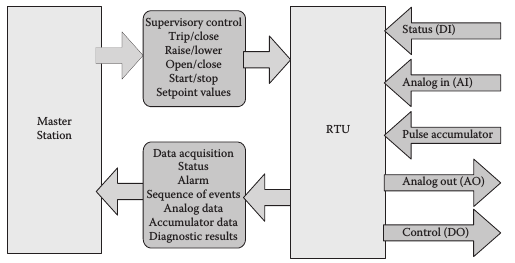
\includegraphics[scale=0.7, natwidth=1003,natheight=490]{imgs/scadadf.png}}
\caption{Architettura SCADA relativa al \emph{data flow}}\label{fig:24}
\end{figure}


\subsubsection{Master station}
Una master station è un sistema di computer responsabile per la comunicazione delle apparecchiature di campo e fornisce un'interfaccia uomo macchina (HMI) nella sala di controllo. In sistemi SCADA molto grandi, la master station può includere server ridondanti, applicazioni distribuite e meccanismi di ripristino. Una grande master station per l'impianto elettrico o \emph{energy management system} (EMS), i figura \ref{fig:25} generalmente ingloba:
\begin{itemize}
	\item Uno o più server di acquisizione dati che si interfacciano con i dispositivi, mediante il sistema di comunicazione;
	\item Server di dati in tempo reale, il quale contiene una base di dati adatta;
	\item Server che funge da storico;
	\item Server per le applicazioni dell'EMS;
	\item Postazioni operativi con HMI.
\end{itemize}    

\begin{figure}[h] \centering{
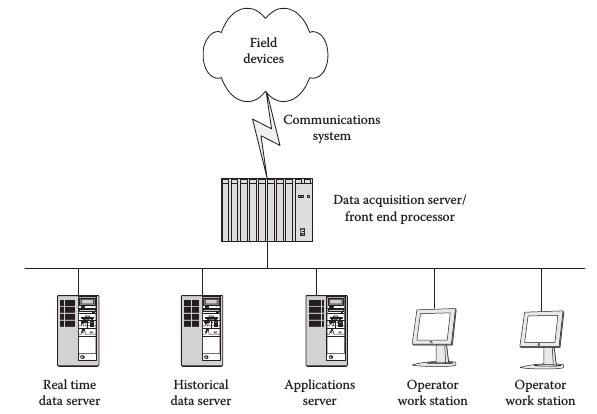
\includegraphics[scale=0.7, natwidth=1003,natheight=490]{imgs/ems.png}}
\caption{Architettura di un EMS}\label{fig:25}
\end{figure}

All'interno dei EMS, le componenti hardware sono connesse mediante LAN. Ci sono diversi tipi di master station, che dipendono dal tipo di funzionalità:
\begin{itemize}
	\item SCADA master station, che effettuano:
	\begin{itemize}
		\item Acquisizione dei dati;
		\item Controllo remoto;
		\item Interfaccia utente;
		\item Analisi dei dati;
		\item Produttore di report;
	\end{itemize}
	\item SCADA master station con controllo di generazione automatico, in aggiunta alla categoria precedente:
	\begin{itemize}
		\item Controllo di gestione automatico;
		\item Economic dispatch;
		\item Scheduling per le transazioni
	\end{itemize}
	\item EMS:
	\begin{itemize}
		\item Configurazione e topologia di rete;
		\item Stima dello stato;
		\item Analisi delle contingenze;
		\item \emph{Optimal power flow};
	\end{itemize}
	\item \emph{Distribution management system} (DMS):
	\begin{itemize}
		\item Interfaccia per la gestione automatizzata per attrezzature o sistema di informazioni geografiche;
		\item Interfaccia per il sistema di informazioni dei clienti;
		\item Interfaccia per la gestione delle interruzioni;
	\end{itemize}	 
	\item \emph{Distribution automation master}:
	\begin{itemize}
		\item Comunicazioni bidirezionali distribuite;
		\item Identificazione, isolamento e ripristino da fallimenti;
		\item Riduzione del voltaggio;
		\item Gestione dei dispositivi che utilizzano energia elettrica;
		\item Controllo del \emph{power factor};
		\item Previsione a breve termine della potenza che sarà consumata.
	\end{itemize}
\end{itemize} 

Tutti i tipi di master station si interfacciano con i dispositivi di campo, tali dispositivi sono RTU o IED.

\subsubsection{Remote Terminal Unit}
Un RTU è un dispositivo basato su microprocessore, che interfaccia un sistema SCADA trasmettendo dati di telemetria alla master station e che cambia lo stato dei dispositivi connessi, in base ai messaggi di controllo ricevuti dalla master station o da comandi generati dallo stesso RTU. Tale dispositivo fornisce dati alla master station e gli consente di emettere comandi per i dispositivi di campo. Tipicamente un  
RTU ha input fisici alle interfacce dei dispositivi di campo ed una  più porte di comunicazione (figura \ref{fig:26}).

\begin{figure}[h] \centering{
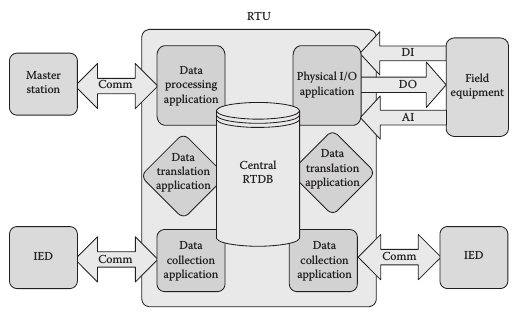
\includegraphics[scale=0.7, natwidth=1003,natheight=490]{imgs/rtu.png}}
\caption{Architettura software di un RTU}\label{fig:26}
\end{figure}

Diversi RTU processano i dati in modi differenti, ma in generale contengono moduli software comuni fra di essi:
\begin{itemize}
	\item Server per i dati real-time;
	\item Applicazioni per l'I/O fisico, che acquisisce i dati dei dispositivi mediante porte;
	\item Applicazioni per l'elaborazione dei dati, da inoltrare ad una master station o HMI;
	\item Applicazioni per la traduzione dei dati, che manipolano i dati prima di presentarli ad una master station.
\end{itemize}

\paragraph{} Le generazioni precedenti di sistemi SCADA generalmente utilizzavano un RTU per ogni substation. Con tale architettura, tutti i cavi delle apparecchiature di campo dovevano terminare all'RTU, il quale offriva capacità limitate di espansione. Per gli ingressi analogici, l'RTU aveva bisogno di un trasduttore per convertire alti livelli di tensione e corrente da CT e PT (current e potential transformation) in milliampere e volt. La maggior parte di RTU avevano una singola porta di comunicazione ed erano capaci di comunicare con una singola master station. La comunicazione fra un RTU e la sua master station era tipicamente ottenuta mediante protocolli proprietari orientati ai bit. Con l'avanzamento della tecnologia gli RTU sono diventati più piccoli e flessibili. Questo ha permesso un approccio verso un'architettura distribuita, con un piccolo RTU per una o più parti dell'attrezzatura di una substation. Questo ha portato una riduzione dei costi di installazione, riducendo i requisiti legati al cablaggio. Questa architettura offre migliori capacità di espansione, mediante l'aggiunta di RTU. Inoltre, la nuova generazione di RTU è capace di accettare direttamente input con alti livelli di corrente alternata, eliminando la necessità di trasduttori e permettendo un collegamento diretto fra CT e PT all'interno degli RTU. Questo ha consentito un aumento delle funzionalità degli RTU, quali registrazione dei guasti e monitoraggio della qualità dell'energia.
\\
Un avanzamento nelle capacità comunicative è stato raggiunto con l'aggiunta di porte disponibile per la comunicazione con gli IED. Tuttavia, il passo avanti più effettivo è stato l'introduzione di protocolli di comunicazione open. La disponibilità di un protocollo di comunicazione open e standard ha offerto la possibilità di scegliere attrezzatura indipendente al venditore per i sistemi SCADA. Lo standard di fatto per i sistemi SCADA per impianti elettrici nel Nord America è diventato DNP3.0, un altro protocollo per l'ambiente manifatturiero industriale è MODBUS. L'ultimo standard di comunicazione adottato è IEC 61850. 
\\
Un'altra tecnologia per i sistemi SCADA sono le comunicazioni di dati della rete. L'architettura di SCADA basata su protocolli di comunicazione seriali pongono  limitazioni sulle capacità del sistema, in quanto:
\begin{itemize}
	\item Esiste un percorso statico tra master e slave che limita la connettività del dispositivo;
	\item Protocolli seriali per SCADA non permettono l'utilizzo di più protocolli su un singolo canale;
	\item Sono presenti problemi con lo scambio di dati con nuove sorgenti;
	\item La gestione della configurazione deve essere eseguita attraverso una porta dedicata alla manutenzione.
\end{itemize}   

L'architettura basata sulla rete offre numerosi vantaggi:
\begin{itemize}
	\item Incremento significativo nella velocità e connettività, una LAN basata su Ethernet incrementa la larghezza di banda disponibile per la comunicazione e il protocollo di rete fornisce un collegamento diretto ai dispositivi presenti nella rete;
	\item Disponibilità di canali logici, protocolli di rete supportano canali logici multipli fra più dispositivi;
	\item Abilità di utilizzare nuove sorgenti di dati, ogni IED può fornire un nuovo numero di porta del protocollo per file o un trasferimento di dati ausiliare, senza disturbare altri processi e aggiunta di ulteriore hardware;
	\item Miglioramento della gestione per la configurazione, eseguita mediante la rete.
\end{itemize}
Tale architettura offre dei tempi di risposta migliori, consente di accedere a dati importanti e riduce i tempi di gestione e configurazione del sistema. Prendendo in esame i passati sistemi SCADA, questi erano semplici sistemi di monitoraggio e controllo remoto che comunicavano mediante link a bassa velocità. Mentre, grazie alla proliferazione di IED basati su microprocessore, è diventato possibile avere informazioni direttamente dai IED, RTU o dalle componenti del sistema di controllo delle substation. Ciò è stato possibile attraverso le capacità di comunicazione degli IED, permettendogli di comunicare con RTU, concentratori di dati o direttamente con la master station. Mentre sempre più IED sono stati installati presso le substation, è divenuto possibile integrare funzionalità di protezione, controllo e acquisizione dati. Molte informazioni precedentemente estratte dagli RTU ora sono fruibili dai IED. Tuttavia non è pratico avere una comunicazione diretta fra master station con i numerosi IED in tutte le substation. Per consentire tale passaggio di dati, un \emph{server della substation} viene utilizzato. Quest'ultimo comunica con tutti gli IED di una substation, conserva tutte le informazioni degli IED, e comunica con la master station centrale. Siccome gli IED utilizzano diversi protocolli di comunicazione, il server della substation deve avere la capacità di comunicare mediante tali protocolli, così come con il protocollo della master station. Tale server permette ad un sistema SCADA di accedere ai dati da diversi IED della substation, il quale prima era possibile solo localmente.
\\
Con l'architettura SCADA basata su server di substation (figura \ref{fig:27}, tutti gli IED (inclusi gli RTU) sono interrogati dal server della substation, mediante la connessione LAN. Con tale architettura, la master station può comunicare direttamente con il server della substation invece che con i RTU e IED. Inoltre, le capacità di comunicazione del server sono superiori rispetto a quelle degli IED, unito al ridotto numero di dispositivi collegati alla master station contribuisce al miglioramento delle performance di comunicazione.

\begin{figure}[h] \centering{
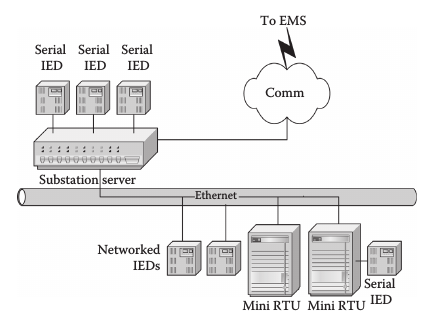
\includegraphics[scale=0.7, natwidth=1003,natheight=490]{imgs/substationserver.png}}
\caption{Architettura di controllo di una substation basata su server}\label{fig:27}
\end{figure}

I dati disponibili nelle substation possono essere di due tipi:
\begin{itemize}
	\item Operazionali o in tempo reale, richiesti per il funzionamento di sistemi di alimentazione e per utilizzare applicazioni di EMS, come controllo di generazione automatico. Tali dati sono memorizzati dalle applicazioni dell'EMS e disponibili come dati appartenente allo storico;
	\item Non operazionali, sono dati appartenenti allo storico ed in generale quei dati usati per analisi, manutenzione e pianificazione. 
\end{itemize} 
I moderni IED, come relè di protezione e misuratori, hanno una quantità enorme di informazioni. Una tipica master station non è progettata per processare questi dati, tuttavia queste informazioni possono essere estremamente utili per utenti diversi. Per poter avvantaggiarsi da questi dati, un meccanismo di estrazione indipendente dalla master station deve essere implementato. I dati operazionali e non hanno meccanismi di raccolta dati diversi, per cui devono esistere due percorsi logici per i dati (figura \ref{fig:28}), uno per gli operazionali che connetta la substation all'EMS, ed un altro per i non operazionali dalla substation a sistemi di information technology. 

\begin{figure}[h] \centering{
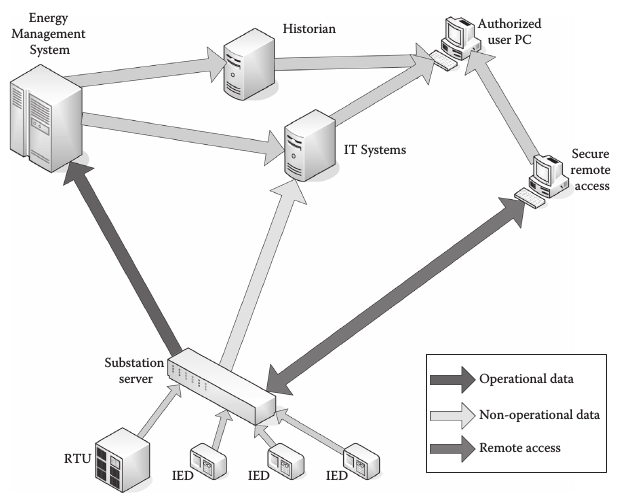
\includegraphics[scale=0.7, natwidth=1003,natheight=490]{imgs/substationdf.png}}
\caption{Scambio di dati delle substation}\label{fig:28}
\end{figure}

Con tutti gli IED connessi ai concentratori di dati delle substation ed un'infrastruttura di comunicazione locale, è diventato possibile avere una connessione  sicura alla maggior parte di IED per effettuare manutenzione remota.
\\ 
Un'architettura di integrazione di substation (figura \ref{fig:29}) offre maggiori funzionalità, avvantaggiandosi di un'architettura del sistema basata su rete, permettendo agli utenti di accedere ad informazioni importanti da tutti i componenti connessi alla rete. Tuttavia, introduce rischi di sicurezza addizionali all'interno del sistema di controllo. Per mitigare tali rischi, una attenzione speciale deve essere presa nella progettazione della rete, concentrandosi sulla sicurezza della rete, implementazioni di autenticazione, autorizzazione e gestione degli utenti. 
 
\begin{figure}[h] \centering{
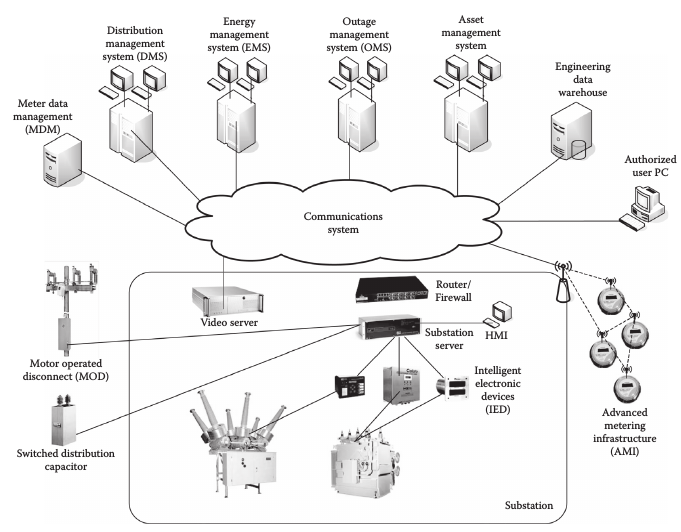
\includegraphics[scale=0.7, natwidth=1003,natheight=490]{imgs/substations.png}}
\caption{Smart substation nell'architettura di una Smart Grid}\label{fig:29}
\end{figure}


\section{Sistemi di trasmissione}
I sistemi di trasmissione si occupano dell'erogazione di energia elettrica. Essi forniscono milioni di megawatt di energia ogni giorno. La domanda di energia sempre crescente ha portato all'evoluzione dei sistemi di trasmissione  dovendo fronteggiare, ad esempio, problemi legati alla variabilità dell'energia prodotta dalle risorse rinnovabili, alle eccessive richieste di energia e all'integrazione con altri sistemi. Sono presenti diverse tecnologie di controllo e monitoraggio che garantiscono efficienza, sicurezza ed affidabilità delle operazioni per quanto riguarda la trasmissione. Alcune di queste tecnologie intraprendono azioni automatiche di controllo della rete ed hanno effetto localmente al punto di connessione, mentre altre possono hanno un ambito operativo che può estendersi fino al centro di controllo. Queste tecnologie offrono controllo dinamico, non solo della fornitura di energia, ma anche della stabilità, voltaggio, frequenze della rete ed altri aspetti.


\paragraph{}Una funzione di base delle reti elettriche è che la quantità di energia prodotta in qualsiasi momento deve corrispondere alla quantità di energia consumata, e questo è compito dell'infrastruttura di trasmissione. Il flusso di energia elettrica attraverso il sistema di trasmissione segue le leggi fondamentali della fisica. Per una data tensione e impedenza di linea, si può calcolare la quantità di corrente che fluirà. Questo flusso di corrente può essere più (sovraccarico) o meno (sottoutilizzato) di quanto desiderato dal gestore di trasmissione. Un dispositivo di trasmissione che è in grado di modificare  la risposta del sistema elettrico ad una data condizione è ovviamente un elemento utile nella creazione di una Smart Grid. L'aggiunta di un simile apparecchio non è sufficiente per ottenere una Smart Grid, ma sono necessari strumenti che consentano di controllare il flusso reale in maniera reattiva di energia, voltaggio, frequenza. Tali dispositivi in ​​grado di mantenere il controllo sul reale flusso di corrente in una linea o nodo o addirittura regione di una rete sono i seguenti:
\begin{itemize}
	\item \emph{Condensatori sincroni}, in grado di controllare la tensione attraverso l'iniezione o l'assorbimento di potenza nei punti chiave del sistema di trasmissione,  consentendo un controllo più preciso del flusso di potenza;
	\item \emph{Flexible AC Trasmission Systems} (FACTS), definito dall'IEEE come "power electronic based system che fornisce il controllo di uno o più parametri del sistema di trasmissione AC per migliorare la controllabilità e aumentare la capacità di trasferimento dell'energia"; 
	\item \emph{High-Voltage Direct Current} (HVDC), sistema di trasmissione di energia elettrica in corrente continua, utilizzato su lunghe distanze. Esso può effettuare un controllo preciso sul flusso di informazioni interno ed esterno, in quanto passano informazioni dettagliate ai centri remoti per monitoraggio, protezione e controllo. Tali sistemi sono in grado di rispondere agli eventi e alle anomalie più velocemente degli operatori, permettendo al sistema di stabilizzarsi e recuperare più velocemente.
\end{itemize}
Questi dispositivi sono in grado di implementare gli aspetti del controllo intelligente, sotto condizioni operative stazionarie normali, così come sotto eventi scaturiti da guasti, e a seconda della loro  velocità di risposta, possono essere in grado di prevenire o accelerare il recupero da situazioni di errore automaticamente. In particolare, FACTS e HVDC forniscono caratteristiche che evitano problemi nei sistemi di alimentazione fortemente caricati; aumentano efficientemente la stabilità e capacità di trasmissione del sistema e aiutano a prevenire disturbi e alterazioni in cascata. Con l'aumento del carico e dei cambiamenti, alcuni elementi del sistema possono andare in contro ai loro limiti termici, e il commercio di energia per ampie aree con diversi modelli di carico contribuiranno ad aumentare la congestione [1,2]. Inoltre, vincoli ambientali, come la minimizzazione delle perdite e riduzione di CO$_2$, avranno un ruolo sempre più importante. Di conseguenza, i progettisti di rete devono affrontare far fronte a conflitti tra la sicurezza delle forniture, sostenibilità ambientale, nonché l'efficienza economica [3,4].
\\
FACTS e HVDC giocano un ruolo importante nelle Smart Grid, permettono infatti di avere reti ibride di AC/DC efficienti e con basse perdite, le quali assicurano migliori gestione del flusso di corrente e prendono parte nel processo di gestione di disturbi e blackout.
\\ 
In aggiunta a questi sistemi relativamente complessi, ci sono altre dispositivi di costo inferiore che aggiungono funzionalità alla Smart Grid, quali monitoraggio dei trasformatori e interruttori, in modo da determinarne l'usura e quindi prevedere i guasti. Tali sistemi prendono il nome di \emph{Wide Area Monitoring, Protection And Control}. Tali sistemi includono l'utilizzo di misurazioni sincronizzate di ampie aree, reti di comunicazione affidabili e ad alta larghezza di banda e schemi di controllo e di protezione avanzati [6].  Un \emph{Phasor Measurement Unit} è il building block basilare di un sistema WAMPAC, il quale converte i segnali semplici dei sistemi di alimentazione in fasori, ovvero rappresentazioni della corrente e del voltaggio, che vengono comparati per ottenere informazioni sullo stato di stress della rete o eventuali alterazioni. Per cui attraverso tali informazioni si riescono ad individuare velocemente alterazioni dei segnali e dove si verificano in maniera accurata, per adottare successivamente misure adeguate.

\section{Sistemi di distribuzione}%practical guidance for defining a smart grid modernization strategy

%http://www.fi-ppp-finseny.eu/wp-content/uploads/2013/05/Future-Internet-for-Smart-Distribution-Systems.pdf
% Yvonne-Anne Pignolet (ABB), Holger Elias (NSN), Timo Kyntäjä (VTT), Ignacio Martín Díaz de Cerio (Iberdrola), Jürgen Heiles (Siemens AG), Didier Boëda (Grenoble INP), Raphael Caire (Grenoble INP): Future Internet for Smart Distribution Systems. Future Network & Mobile Summit 2012.  http://www.fi-ppp-finseny.eu/publications/

Il sistema di distribuzione è il cuore di una Smart Grid. I progressi nelle tecnologie di controllo e comunicazione hanno consentito il funzionamento remoto automatico e/o semi-automatico delle componenti del sistema di distribuzione, che nel passato poteva essere azionato solo manualmente. 
%Gli sforzi di un sistema distribuito sono sempre stati concentrati su:
%\begin{itemize}
%	\item Mantenere condizioni accettabili dei componenti di distribuzione;
%	\item Minimizzare le perdite di corrente elettrica;
%	\item Proteggere il sistema da eventuali corti circuiti, picchi e cali di tensione;
%	\item Fornire misure di sicurezza per il sistema elettrico ed gli utenti.  
%\end{itemize}
La necessità di lavori manuali da parte degli operatori nelle substation di distribuzione fu eliminata dall'applicazione di IED, sistemi SCADA e logger automatici di dati. In seguito, furono aggiunti strumenti, indicati come \emph{fault location isolation and service restoration} (FLISR), per il ripristino energetico per fa fronte a corti circuiti e malfunzionamenti temporanei. Successivamente,  per il controllo e monitoraggio remoto degli alimentatori furono sviluppati sistemi con controllo del \emph{volt/VAr} (vedi ...) e SCADA basati su FLISR per migliorare l'affidabilità e ridurre le perdite di energia. Anche se la maggior parte dell'energia veniva fornita da grandi generatori centrali, un numero crescente di generatori distribuiti faceva il suo ingresso nel sistema di distribuzione, tra cui le risorse energetiche rinnovabili e nello stesso periodo ci furono introdotti i sistemi AMR, in grado di effettuare comunicazioni unidirezionali. Progressivamente, le risorse energetiche rinnovabili costituiscono attualmente un importante aspetto della Smart Grid. Il sistema di distribuzione, infatti, deve fronteggiare l'alta variabilità delle risorse rinnovabili. Ad esempio, l'alta nuvolosità e la scarsa potenza del vento causano una riduzione dell'energia prodotta, che deve essere compensata mediante condensatori e regolatori di voltaggio. Inoltre per contrastare le variabilità della generazione energetica distribuita, le unità di quest'ultima sono equipaggiate di convertitori di corrente da diretta ad alternata per fornire in maniera reattiva energia, riducendo l'energia persa e migliorando il \emph{power factor}, ovvero il rapporto tra potenza necessaria per compiere lavoro e quella erogata. La generazione di energia distribuita unita alla conservazione dell'energia e ai sistemi di controllo avanzati consentono alle microgrid isolate di continuare a servire i clienti nelle comunità locali, sia quando la microgrid si separa dalla rete che si verifica una mancanza di corrente. 
\\ 
Il sistema di distribuzione si avvale di un \emph{distribution management system} (DMS), per la gestione e prendere decisioni e di sistemi con comunicazione bidirezionale, \emph{advanced metering infrastructure} (AMI), per supportare una vasta gamma di applicazioni collegate al fatturato e fornire informazioni in tempo reale sul consumo dei clienti e sulle condizioni delle apparecchiature elettrice di distribuzione. I sistemi AMI permettono programmi di \emph{demand-side management} (DSM), per ad esempio gestire dei picchi energetici. I sistemi AMI e sensori intelligenti dentro e fuori le substation, tramite comunicazioni ad alta larghezza di banda consentono di ottenere una grande quantità di informazioni proveniente dalle componenti del sistema di distribuzione. In aggiunta alle informazioni in tempo reale da collezionare, è presente una moltitudine di informazioni geo-spaziali, che vengono memorizzati in \emph{geographic information system} (GIS). Tale abbondanza di dati contiene informazioni aiutano nella gestione del sistema di distribuzione ed è complessa da analizzare, per cui non vengono utilizzati strumenti tradizionali, ma strumenti per l'analisi dei dati specifici [].    
 
\subsection{Distribution Management System}
Il sistema di distribuzione della Smart Grid si affida ad un sistema con una visione completa sulle condizioni dei sistemi di alimentazione, ossia il distribution management system (figura \ref{fig:2_10}). 

\begin{figure}[h] \centering{
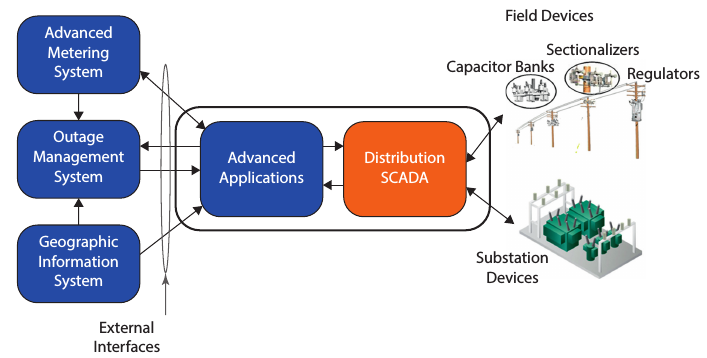
\includegraphics[scale=0.7, natwidth=1003,natheight=490]{imgs/dmshigh.png}}
\caption{Configurazione ad alto liveo livello di un Distribution Management System}\label{fig:2_10}
\end{figure}

Un DMS integra il monitoraggio, l'analisi di rete e le applicazioni di controllo in un sistema decisionale, in grado di gestire le complessità del sistema di distribuzione, sia in condizioni stazionarie che di emergenza. Migliorare l'affidabilità e la qualità del servizio in termini di riduzione delle interruzioni, minimizzando il tempo di interruzione e mantenendo i livelli di frequenza e di tensione accettabili.  
La figura \ref{fig:2_11} mostra l'architettura di un DMS.

\begin{figure}[h] \centering{
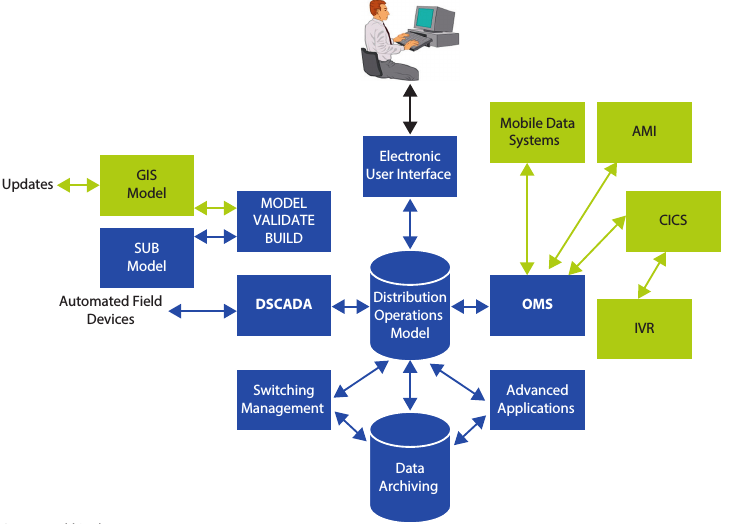
\includegraphics[scale=0.7, natwidth=1003,natheight=490]{imgs/dms.png}}
\caption{Architettura di un Distribution Management System}\label{fig:2_11}
\end{figure}

Uno dei sistemi chiave nel moderno centro di controllo è l'Outage Management System (OMS), che assiste nella gestione del sistema di distribuzione elettrica nel rilevare interruzioni di alimentazione, determinare la posizione approssimativa della causa principale dell'interruzione, stimare il tempo di ripristino, valutare i danni e attività di restauro, e lo sviluppo di statistiche relative alle interruzioni. Il DMS deve essere in grado di rappresentare tutti gli aspetti della rete di distribuzione, inclusi conduttori, trasformatori, interruttori manuali o automatici e tutti gli altri dispositivi che operano nel sistema di distribuzione. Per poter effettuare politiche di bilanciamento del carico e gestire le variabilità energetiche nel sistema di distribuzione, un algoritmo \emph{load-flow}, il quale permette di calcolare i parametri della rete in ogni punto della rete, deve essere eseguito su dati telemetrici, resi disponibili dai sistemi SCADA e la telemetria ad essi associata, mediante la tecnologia AMI e l'OMS. 
\\
Con un modello di rete complesso, quantità significanti di dati telemetrici e calcolati, risulta cruciale fornire visualizzazione dei risultati. Un DMS deve mostrare i dati delle rete in viste geografiche, come mappe, schematiche e diagrammi. 
\\
La \emph{Demand response} è una funzione chiave per il DMS per ridurre i picchi di consumo energetico. Per modificare le abitudini dei consumatori, soprattutto nelle ore di punta, le società di servizi offrono diverse politiche di pagamento, incentivando i clienti ad usufruire dell'energia nelle ore notturne. Siccome questo approccio non fornisce sufficienti riduzioni, il DMS può aiutare in questa direzione riducendo la tensione erogata, grazie alle funzionalità dei volt/VAr, tra 3 e 7\%, senza che i clienti ne siano consapevoli.







% [1,2] [3,4] trasmissione

% [6] V. Terzija, G. Valerde, D. Cai, P. Regulski, V. Madani, J. Fitch, S. Skok, Miroslav M. Begovic and A. Phadke, “Wide-Area Monitoring, Protection and Control of Future Electric Power Networks”, IEEE Proceedings, vol. 99, No.1, pp. 80-93, January. 2011 

%[7]  Federal Energy Regulatory Commission Assessment of Demand Response & Advanced Metering http://www.ferc.gov/legal/staff-reports/12-08-demand-response.pdf

% [8] McKerracher, C. and Torriti, J. (2013) Energy consumption feedback in perspective: integrating Australian data to meta-analyses on in-home displays. Energy Efficiency, Volume 6 (2). pp 387-405

% Proposed terms and definitions for flexible AC transmission system(FACTS), IEEE Transactions on Power Delivery, Volume 12, Issue 4, October 1997, pp. 1848–1853

% http://ieeexplore.ieee.org/stamp/stamp.jsp?tp=&arnumber=6298960 

%http://www.smartgridinformation.info/pdf/5264_doc_1.pdf

% http://www.cs.nmsu.edu/~misra/papers/SmartGridSurvey.pdf


%libri 


\chapter{Smart Grid Cybersecurity}
%\chapter{Smart Grid Cybersecurity: requisiti, building blocks e potenziali minacce}
Il termine \textbf{``sicurezza"} si riferisce alle tecniche, ai processi e ai provvedimenti adottati per proteggere dati, reti di comunicazione, tecnologie informatiche e sistemi di calcolo da attacchi o da accessi non autorizzati. \newline
L'approccio tradizionale prevede che la maggior parte delle risorse a disposizione per mettere in sicurezza il sistema si focalizzi sulle componenti più cruciali e che le protegga dalle minacce più grandi e più note; questo meccanismo fa si che le componenti secondarie siano indifese e, inoltre, non protette da attacchi meno pericolosi. Tale approccio, però, risulta inefficiente nell'ambito della Smart Grid. \newline Per adattarsi al nuovo sistema, le organizzazioni promuovono un metodo più proattivo ed adattivo: il NIST, per esempio, ha recentemente pubblicato delle linee guida che consigliano uno spostamento verso il continuo monitoraggio e verso valutazioni real-time \cite{smartgrids}.\newline \newline
La sicurezza della Smart Grid, in relazione al suo sviluppo, è un tema fortemente discusso: tutti concordano nel sostenere che la Smart Grid dovrebbe avere un modello di sicurezza robusto; il problema è che ci si trova dinanzi a due sfide: come poter rispondere ai requisiti richiesti e come poter applicare le numerose alternative esistenti quando si cerca di rendere sicuro un ambiente complesso come la Smart Grid.
\newline \newline
Quando si sente parlare di ``nuova tecnologia", di ``interconnessione" e di ``condivisione dei dati", subito ci si focalizza sui benefici e sulle nuove funzionalità che tali concetti portano con loro. C'è da considerare, però, anche i nuovi rischi che queste nuove funzionalità introducono all'interno del sistema.\newline Per questo motivo, lo scopo della sicurezza è quello di garantire che le funzionalità del sistema operino correttamente e siano protette da abusi. È importante sottolineare, però, che non esistono applicazioni, reti o sistemi completamente sicuri e le Smart Grid non sono un'eccezione. Sebbene ogni componente della nuova rete elettrica porti con se numerosi miglioramenti operazionali  o funzionali, introduce anche nuove vulnerabilità e rischi addizionali che, se non propriamente gestiti, possono portare il sistema ad essere esposto ad attacchi di varia natura.
\section{Cenni storici}

\section{Definire la sicurezza}
La sicurezza tradizionale fa affidamento sulla cosiddetta \textbf{CIA triad}, che ne costituisce il cuore. La CIA triad comprende tre concetti: \emph{confidentiality}, \emph{integrity} ed \emph{availability}. \newline Una concezione più moderna, e più adatta all'ambiente della Smart Grid, prevede l'utilizzo del \textbf{Parkerian hexad}, figura \ref{fig:31}, proposto da Parker nel 2002. Tale modello propone, in aggiunta ai tre classici concetti precedenti, altri tre principi: \emph{control} (o \emph{possession}), \emph{authenticity} ed \emph{usability} (o \emph{utility}). \newline All'interno di questi sei pilastri, è possibile trovare tutti i problemi relativi alla Smart Grid \cite{smartgrids}.
\begin{figure}[h]\centering{
  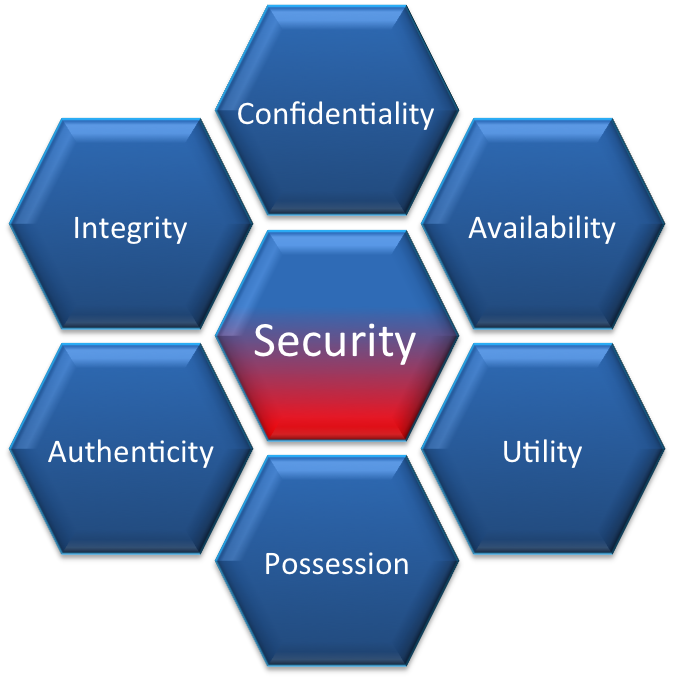
\includegraphics[scale=0.5, natwidth=674,natheight=679]{imgs/hexad.png}
  \caption{Parkerian hexad}\label{fig:31}
}
\end{figure}
\subsection{Confidentiality}
Tale concetto porta con sé una serie di problemi e di preoccupazioni relative alla trasmissione e alla memorizzazione di dati ricavati dalle operazioni della Smart Grid. Questo tipo di dati, infatti, è spesso ritenuto \textit{confidenziale}, nel senso che se fosse noto, avrebbe tutto il potenziale per causare danni alla sicurezza delle operazioni di tutto il sistema. \newline La confidenzialità, inoltre, può essere intesa anche in un'altra accezione: se i dati fossero noti alla concorrenza, per esempio,  quest'ultima potrebbe trarre un notevole vantaggio in uno specifico settore o in tutto il mercato. \newline A tali fattori si aggiungono altre nuove problematiche legate alla \textit{privacy del consumatore} e, quindi, dei suoi dati, che vengono fuori da meccanismi di metering quali l'AMI. Gli utenti, infatti, si aspettano che i consumi relativi alle loro abitazioni private rimangano confidenziali; se così non fosse, la disponibilità di tali informazioni insieme alla capacità di fare data mining, avrebbe il potenziale per creare significative preoccupazioni sulla privacy. \newline I punti della Smart Grid che introducono rischi per la confidenzialità, sono costituiti da tutte le locazioni in cui sono memorizzati i dati e da tutti i meccanismi di trasmissione delle informazioni. Per quanto riguarda i dati memorizzati, questi potrebbero essere letti, copiati e distribuiti a soggetti diversi dai destinatari. Per quanto riguarda la trasmissione, invece, sia su reti private che su reti pubbliche come Internet, i dati potrebbero essere intercettati, copiati e distribuiti. \newline La soluzione a tali problemi risiede nelle funzioni di \textit{cifratura dei dati} e di \textit{controllo degli accessi}. Fornendo l'appropriato livello di cifratura delle informazioni, quest'ultime possono essere protette da chiunque non sia il diretto destinatario. \newline Il controllo degli accessi, prevede che i dati siano protetti da coloro che hanno l'autorizzazione per accedere al sistema ma che, allo stesso tempo, non hanno bisogno di tali dati per svolgere il loro lavoro.

\subsection{Integrity}
L'integrity si riferisce all'abilità del sistema di evitare che le informazioni possano essere modificate da persone o da sistemi non autorizzati. \newline Se si rendono possibili meccanismi di modifica volontari quali la manipolazione dei dati, o anche involontari quali la loro corruzione, i sistemi riceveranno informazioni non accurate; a lungo andare ciò potrebbe avere un impatto negativo su tutte le operazioni e, in casi estremi, portare ad instabilità o compromettere del tutto la Smart Grid. \newline
I punti della nuova rete elettrica che introducono rischi per l'integrità, sono tutti quei punti che consentono il passaggio dei dati da un sistema ad un altro. Pertanto, la sicurezza di tali meccanismi di transizione è importante, ma ancora più importante è come il sistema che riceve i dati possa assicurarsi della validità di quest'ultimi: se i dati subiscono manipolazioni mentre sono in viaggio tra i due sistemi, il ricevente potrebbe prendere decisioni basate su tali informazioni (che risultano essere errate); se, invece, i dati sono soggetti a corruzione durante la loro transizione, ci si potrebbe trovare di fronte ad un comportamento inaspettato del ricevente. In entrambi i casi, è evidente che l'integrità dei dati sia cruciale per assicurare la stabilità delle operazioni.   \newline
Le risposte ai problemi di integrità, possono essere trovate nei meccanismi di \textit{auditing}, di \textit{authorization}, di \textit{nonrepudiation}, e di \textit{message-signing}, che saranno trattati in seguito (vedi paragrafo 3.3, building blocks).


\subsection{Availability}
Molto spesso si tende ad utilizzare i concetti di reliability ed availability in maniera intercambiabile; in realtà, tali concetti hanno due significati diversi. La reliability, infatti, risponde alle seguenti domande: ``quanto spesso fallisce il sistema?", ``quanto è elastico?"; l'availability, invece, indica la disponibilità del sistema e, quindi, la capacità di compiere il lavoro che gli è stato assegnato, \textit{nel momento in cui se ne ha bisogno}. \newline Una porzione del sistema potrebbe essere attiva, eseguendo e processando i comandi, il 100\% del tempo, e pertanto molto affidabile ma, se le performance non sono adeguate ai bisogni della rete e operazioni critiche vengono ritardate o mancano, non si può dire che il sistema sia disponibile. \newline
I punti della Smart Grid che introducono rischi per la disponibilità sono troppi per poterli elencare: qualsiasi sistema, rete, dispositivo che gestisce le comunicazioni, processo per la gestione dei messaggi, e qualsiasi servizio invocato a qualsiasi livello applicativo e il suo sistema operativo sottostante sono un rischio per la disponibilità quando si trovano a dover gestire l'inoltro di un comando da un'estremità del sistema ad un'altra. Risolvere tale rischio è quasi tanto complicato quanto identificare le componenti del sistema che hanno il potenziale per impattare sulla disponibilità. La maggior parte delle soluzioni si affida a tecniche di ridondanza (clustering, bilanciamento del carico); il costo di tali metodologie, però, cresce in maniera proporzionale ai punti di fallimento che si identificano nel sistema. 

\subsection{Control}
La capacità di controllare le informazioni che necessitano protezione è essenziale per assicurare la loro integrità e la loro usabilità a lungo termine. Ciò ha diverse implicazioni per tutti quei sistemi che si affidano al meccanismo di controllo per scopi di vario genere (legali, normativi o commerciali): se le informazioni utilizzate per calcoli finanziari, come ad esempio i dati ricavati da meccanismi di metering, non fossero controllate, potrebbero compromettere tutti i sistemi che le forniscono e le trasmettono; di conseguenza, la provenienza di tali informazioni non potrebbe essere più garantita, portando una diminuzione dell'affidabilità di quest'ultime. 

\subsection{Authenticity}
Tale termine è spesso utilizzato per descrivere la certezza della provenienza. Il processo di verifica dell'autenticità è simile al processo utilizzato per verificare l'integrità: assicurarsi che la fonte dei dati e i dati stessi, siano autentici.

\subsection{Usability}
Questo aspetto del Parkerian hexad si preoccupa di assicurare che i dati siano utilizzabili. \newline Consideriamo un flusso di dati opportunamente cifrato: quest'ultimo garantisce la sicurezza delle informazioni, ma rende molto difficile far si che queste ultime siano utili. L'usabilità è il fattore che, in definitiva, fornisce valore a livello aziendale e pertanto deve essere preservato e trattato come il requisito con più alta priorità. 

\subsection{Analisi dei rischi}
Quale sarebbe il rischio per l'intero sistema Smart Grid se il sistema stesso, o qualsiasi sua componente, fosse compromessa? Tale rischio e il suo potenziale costo, guidano il lato economico delle decisioni per la progettazione dei meccanismi di sicurezza. \newline Come determinare l'accettazione dei rischi è, pertanto, una decisione legata al business e non una decisione tecnica. Un'azienda che sceglie di adottare una particolare metodologia per l'analisi dei rischi, avrà come input le proprie variabili che guidano le decisioni; tali variabili sono solitamente legate ad un rischio finanziario che l'azienda assume basandosi su una propria analisi competitiva del mercato o su condizioni regolamentari sotto le quali opera. \newline Ci sono altre motivazioni, oltre a quelle finanziarie, che possono guidare l'accettazione dei rischi, come ad esempio fattori legislativi o legati a normative industriali: tali fattori possono portare ad adottare comportamenti che garantiscono la sicurezza anche in assenza di forti incentivi economici, per aggiungere ulteriori capacità di protezione del sistema. \newline È importante riconoscere che nessuna decisione riguardante la sicurezza dovrebbe essere presa senza prima aver considerato i rischi: ``dove sono i rischi nel sistema?", ``Quanto costerà un fallimento del sistema?", ``Quanto costerà un fallimento della sicurezza del sistema?". Un'azienda dovrebbe essere in grado di capire i rischi e dovrebbe essere capace di fare scelte informate ed intelligenti su come risolvere tali problemi. 


\section{Building blocks}
Nel paragrafo precedente, sono state descritte una serie di potenziali minacce e funzioni di sicurezza che sono importanti per sistemi complessi ed interdipendenti come le Smart Grid. \newline In questo paragrafo, si esaminerà una possibile architettura di sicurezza che comprende tutte le funzioni precedentemente analizzate e che cerca di creare una struttura adatta a risolvere tutte le vulnerabilità descritte nel paragrafo 3.2.

\subsection{Layered Security Model}
Il concetto di modello di sicurezza \textit{stratificato} non è un concetto nuovo: i sistemi operativi ed i microprocessori, infatti, lo utilizzano da tempo per controllare gli accessi a  risorse privilegiate. \newline Immaginare tale concetto applicato ad una Smart Grid non è difficile. \newline Dalla figura \ref{fig:32} è possibile vedere che la struttura di tale modello è una struttura ad anello in cui la comunicazione tra gli strati del sistema è sicura. In generale, uno strato esterno non può avere libero accesso alle risorse presenti su uno strato più interno; inoltre, le richieste per le risorse non dovrebbero essere in grado di ``saltare" i vari anelli: una richiesta che parte dal terzo anello, non dovrebbe poter accedere direttamente alla risorsa del primo, ma gli accessi sono regolati da opportune interfacce progettate in modo tale da assicurare la sicurezza di tutto il sistema.

\begin{figure}[h]\centering{
  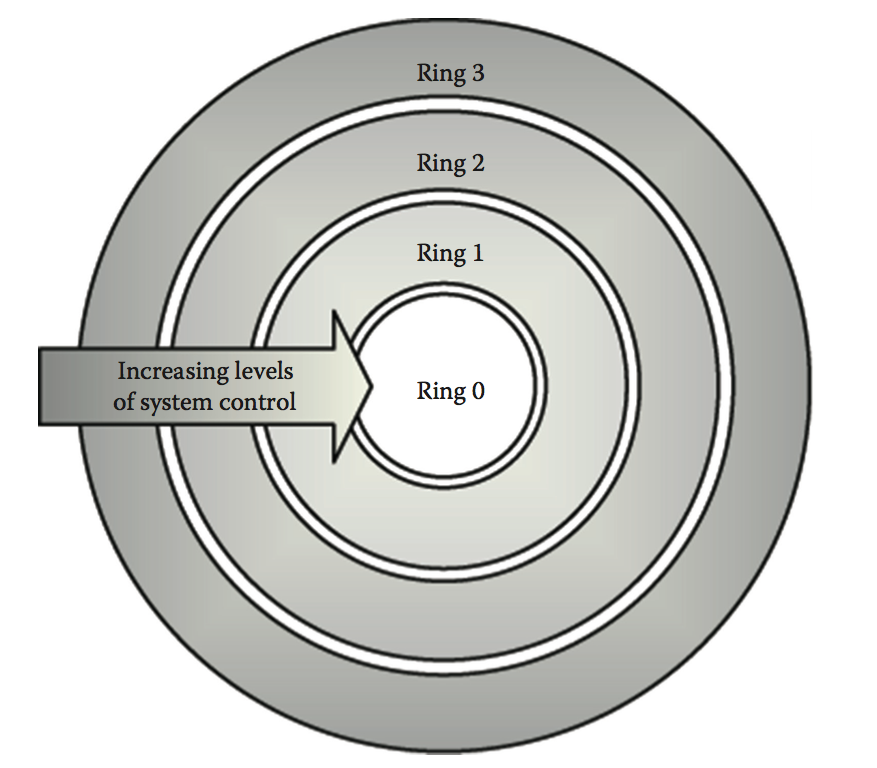
\includegraphics[scale=0.25, natwidth=877,natheight=768]{imgs/ring.png}
  \caption{Layered security model}\label{fig:32}
}
\end{figure}

Una Smart Grid ben progettata, dovrebbe essere in grado di offrire una simile protezione: i sistemi e le risorse poste agli estremi, come ad esempio dispositivi HAN (home area network) o smart meter, non dovrebbero avere la possibilità di accedere direttamente agli strati operativi (ring 0) della Smart Grid e, in più, i dati che passano per il sistema dovrebbero attraversare opportune interfacce che ne assicurino l'integrità prima di procedere verso strati più interni. \newline
Indipendentemente dal meccanismo specifico utilizzato per separare gli strati, ci sono diversi principi architetturali chiave che dovrebbero essere considerati nel percorso dei dati tra gli anelli: il primo e il più importante è assicurarsi che un fallimento in uno strato non abbia impatto né in uno strato più basso né in qualsiasi sistema dello stesso strato. Con il termine ``impatto" ci si riferisce al fatto che nessuna tra confidentiality, integrity, o availability degli strati sottostanti debba essere colpita. È importante notare, però, che il viceversa non è vero: molto spesso danni ai livelli più bassi si propagano verso gli strati superiori e ciò è dovuto alla natura gerarchica del sistema.
\newline \newline 
Nelle prossime sezioni si analizzano le principali funzioni che costituiscono le componenti di sicurezza di alto livello che la Smart Grid dovrebbe avere per assicurare la protezione del sistema.

\subsection{Authentication}
L'autenticazione è il processo di verifica dell'identità di una persona o di un servizio che richiede l'accesso ad una risorsa. \newline Un meccanismo di autenticazione robusto potrebbe richiedere un certo numero di componenti, ognuna delle quali offre una particolare funzione di tutto il processo. \newline Spesso si tende a pensare all'autenticazione in termini di username e password, il che è corretto, ma non è solo questo: vi può essere autenticazione anche tra sistemi, processi o componenti hardware. Ci sono due componenti base per un meccanismo di autenticazione:
\begin{itemize}
\item \textit{Identity Database}, contiene le informazioni necessarie per determinare chi e cosa sta tentando di accedere al sistema;
\item \textit{Identity Management System}, repository centrale di tutte le risorse che richiedono servizi di autenticazione.
\end{itemize}

\subsection{Authorization}
L'autorizzazione è il processo che verifica ciò che la persona o il servizio autenticato può fare all'interno del contesto del sistema. \newline 
Spesso i sistemi più semplici prevedono solo due modalità: ``read-write" e ``write-only"; i sistemi più complessi, invece, dovrebbero fornire regole di autorizzazione più specifiche, includendo la possibilità di indicare quali campi si possono modificare e quali no, solo ad un certo orario del giorno e solamente se autenticati su specifiche macchine.

\subsection{Auditing}
Il cuore di una qualsiasi analisi dei rischi è costituito dal programma di controllo. Senza revisioni periodiche dell'efficacia dei meccanismi di sicurezza che sono in atto nella Smart Grid, non ci sarebbe nessuna garanzia che il sistema sia sicuro. \newline
Un buon programma di controllo dovrebbe essere eseguito periodicamente e dovrebbe testare quelle componenti che sono ritenute essenziali dall'azienda per mettere in sicurezza le operazioni del sistema. Tra i meccanismi più utili per eseguire tali revisioni, vi sono i seguenti:
\begin{itemize}
\item \textit{Logging}: utilizzare file di log e memorizzare al loro interno tutti gli accessi critici al sistema e tutti i cambiamenti avvenuti;
\item \textit{Time Synchronization}: in un sistema unificato come una Smart Grid, è essenziale che tutti i dispositivi condividano lo stesso tempo.
\end{itemize}

\subsection{Key Management}
È il processo che gestisce le emissioni delle chiavi per utenti, applicazioni e dispositivi. Tali chiavi sono utilizzate per stabilire l'identità e per assicurare l'integrità dei messaggi quando si inviano comandi tra sistemi. \newline 
Se consideriamo centinaia di chiavi, la loro gestione è relativamente semplice; ma quando ci si trova di fronte a centinaia di migliaia, o addirittura milioni, di dispositivi, la gestione diventa più complessa. Ogni chiave nel sistema sia relativa ad applicazioni, al sistema, ad un dispositivo o ad una persona, dovrebbe poter essere modificata o revocata su richiesta. 
\newline Per fare ciò, si utilizza la ben nota \textit{Public Key Infrastructure} (PKI) \cite{smartgrid}.

\subsection{Message Integrity}
Per trattare l'integrità dei messaggi, consideriamo tre meccanismi: signing, nonrepudiation ed encryption. \newline
Per quanto riguarda il meccanismo di \textit{signing}, quando un messaggio viene inviato da un sistema ad un altro, vi è prima un processo di autenticazione per dimostrare un'identità, seguito da un processo di autorizzazione, per verificare ciò che l'identità può fare. Una volta effettuati questi due controlli, può iniziare lo scambio di messaggi tra i due sistemi. Ci sono due motivazioni principali per cui conviene firmare un messaggio: la prima è assicurare che il contenuto del messaggio non sia stato modificato durante la trasmissione tra i sistemi; la seconda è permettere di verificare l'identità del mittente indipendentemente dal processo di autenticazione. \newline
La \textit{nonrepudiation} entra in gioco quando il mittente di un messaggio necessita di essere riconosciuto (o confermato). Tale termine, infatti, si riferisce alla capacità di fornire una prova inconfutabile, ad una terza parte, di chi ha iniziato una certa azione nel sistema, anche se la persona in questione non sta partecipando al momento. \newline
Il termine \textit{encryption} porta con sé una serie di problematiche e di discussioni ampiamente trattate in letteratura, pertanto è impossibile riassumerlo in poche righe. Si può, però, riassumere il suo scopo: assicurarsi che un messaggio non possa essere letto da una persona o da un sistema che non sono i diretti destinatari dell'informazione. Ciò può essere messo in pratica attraverso innumerevoli algoritmi di cifratura, i quali fanno affidamento sul preservare l'integrità della chiave utilizzata per cifrare i dati; pertanto se tale chiave viene compromessa, lo sarà anche il messaggio. 

\subsection{Network Integrity}
Vi è un'infinità di modi per garantire l'integrità di rete, ognuno dei quali dipende dai dispositivi che la compongono e dalle loro necessità. Infatti, poiché ogni rete ha bisogni diversi, non vi è una configurazione che sia adatta a tutte quante.
\newline Due dei meccanismi principali sono i seguenti:
\begin{itemize}
\item \textit{Firewall}, utilizzato per restringere il traffico sulla rete ad uno specifico insieme di regole. Per esempio, potrebbe limitare il traffico a specifici canali di comunicazione tra un dispositivo e un insieme noto di altri dispositivi;
\item \textit{Rilevamento e prevenzione delle intrusioni}, messo in atto analizzando il traffico della rete per identificare specifici pattern di dati che corrispondono ad attacchi noti.
\end{itemize}

\subsection{System Integrity}
\begin{itemize}
\item \textit{Protezione da malware}, o più comunemente nota come protezione antivirus: ogni sistema dovrebbe avere una strategia che lo protegga da questo tipo di minacce; una protezione robusta, infatti, non solo può evitare che file maliziosi vengano memorizzati, ma può anche far si che si possa avvisare un operatore del ritrovamento del malware;
\item \textit{Gestione della configurazione del sistema}: le specifiche su come un sistema è configurato possono impattare enormemente sulla sua sicurezza. La gestione è necessaria per assicurarsi che il sistema non cambi rispetto alle basi di funzionamento stabilite;
\item \textit{Validazione e testing}: essenziali per garantire l'integrità del sistema. Prima di effettuare qualsiasi cambiamento e di distribuire nuovi sistemi, bisogna valutare le nuove modifiche e capire che impatto hanno sull'intero sistema. I cambiamenti devono essere testati per sicurezza e per garantire che non abbiano conseguenze negative sull'affidabilità di tutto il sistema.
\end{itemize}

\section{Minacce e loro impatto}

\section{Compagnie}

\section{Servizi di terze parti}


\chapter{Standard e tecnologie \label{chap:chap5}}
L'infrastruttura di comunicazione consiste tipicamente di sistemi SCADA con canali di comunicazione dedicati da e verso il centro di controllo del sistema e di una Wide Area Network (WAN). I sistemi SCADA collegano tutte le principali strutture operative del sistema mentre la WAN è prevalentemente usata per azioni di mercato. Uno sviluppo importante per la Smart Grid (vedi Figura \ref{fig:cisg}) è quello di estendere la comunicazione a tutto il sistema di distribuzione e di stabilire una comunicazione bidirezionale con i clienti attraverso le Neighbourhood Area Network (NANs) che coprono le zone servite dalle sottostazioni di distribuzione. I clienti avranno la necessità di una Home Area Network (HAN) a cui saranno connessi gli smart device.
\begin{figure}[h]
	\centering
	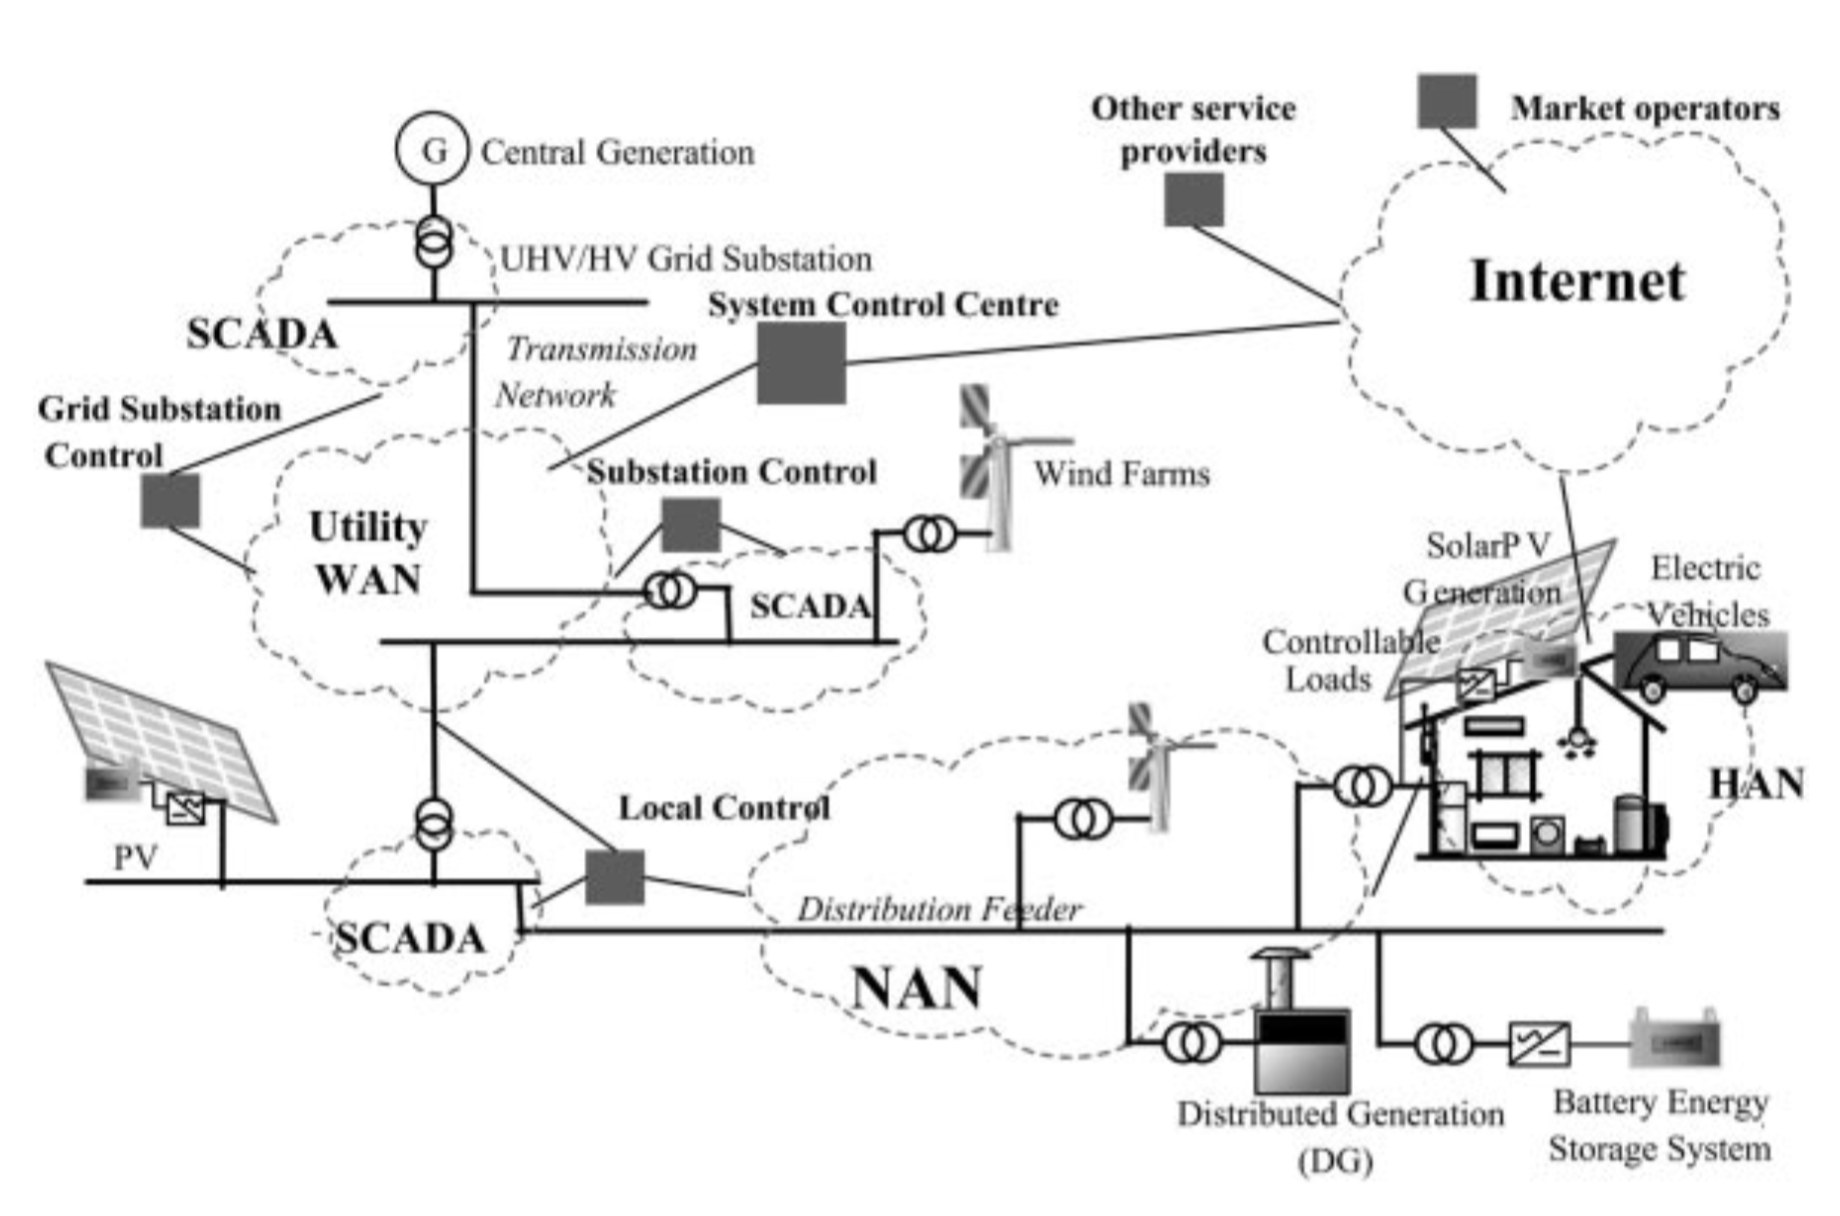
\includegraphics[scale=0.310]{imgs/comm_inf_SG.png}
	\caption{Una possibile infrastruttura di comunicazione per la Smart Grid} \label{fig:cisg}
\end{figure}\\
Le sotto-reti di comunicazione che andranno a comporre la Smart Grid utilizzano diverse tecnologie (vedi Figura \ref{fig:th}) e di particolare interesse è il modo in cui quest'ultime possono essere integrate in maniera efficace. Le Smart Grid possono utilizzare diverse tecnologie di comunicazione wired e wireless (cellulare, satellitare, microwave, WiMAX etc.). Le tecnologie di comunicazione wireless short range, come WiFi e ZigBee,  sono tipicamente utilizzate nelle HAN.
In questo capitolo, saranno descritte alcune tecnologie di comunicazione associate ai livelli inferiori del modello di riferimento ISO/OSI.
\begin{figure}[h]
	\centering
	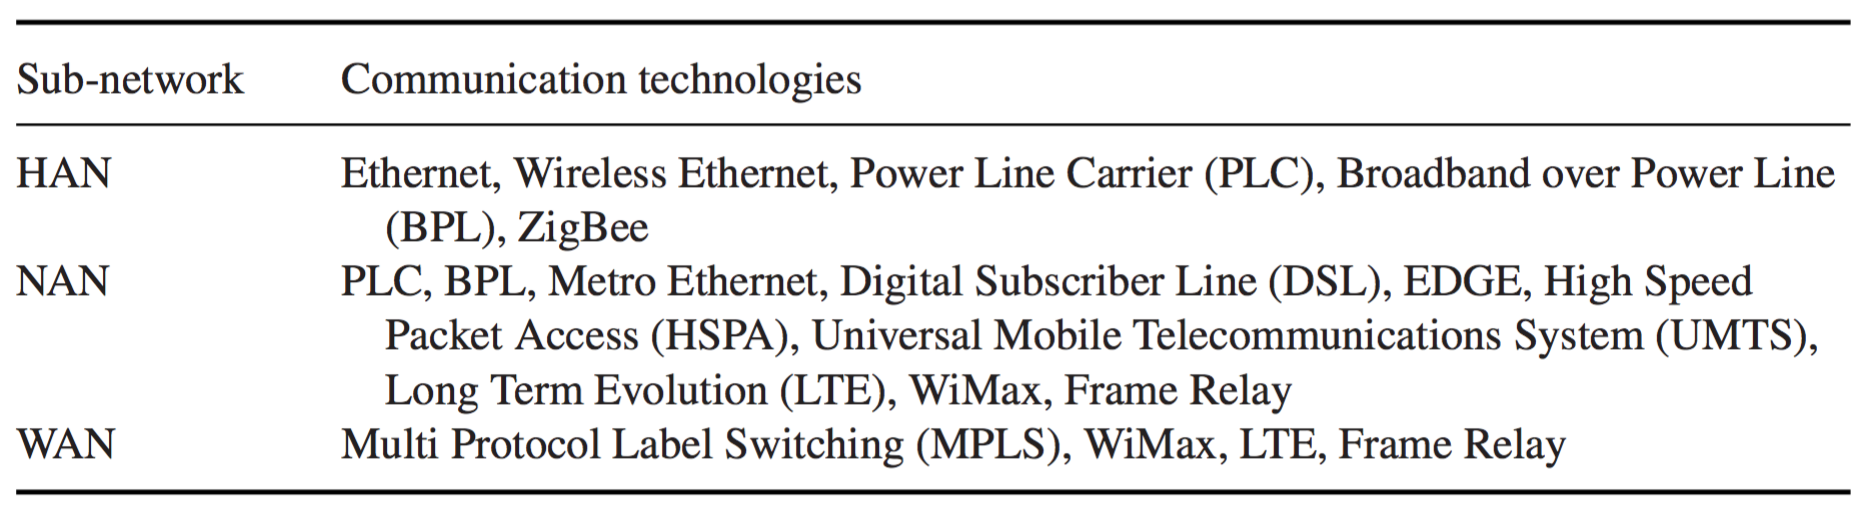
\includegraphics[scale=0.350]{imgs/tech.png}
	\caption{Tecnologie usate nelle differenti sottoreti} \label{fig:th}
\end{figure}

\section{Tecnologie di comunicazione}
\subsection{IEEE 802}
IEEE 802 è una famiglia di standard sviluppati per il supporto alle reti locali (LAN). Facendo riferimento alla Smart Grid, tali standard sono applicabili alle reti LAN in sistemi SCADA, NAN per le reti di distribuzione e HAN nei locali dei clienti. La Figura \ref{fig:arch_802} mostra come l'architettura IEEE 802 è incentrata sui due livelli inferiori del modello ISO/OSI.
\begin{figure}[h]
	\centering
	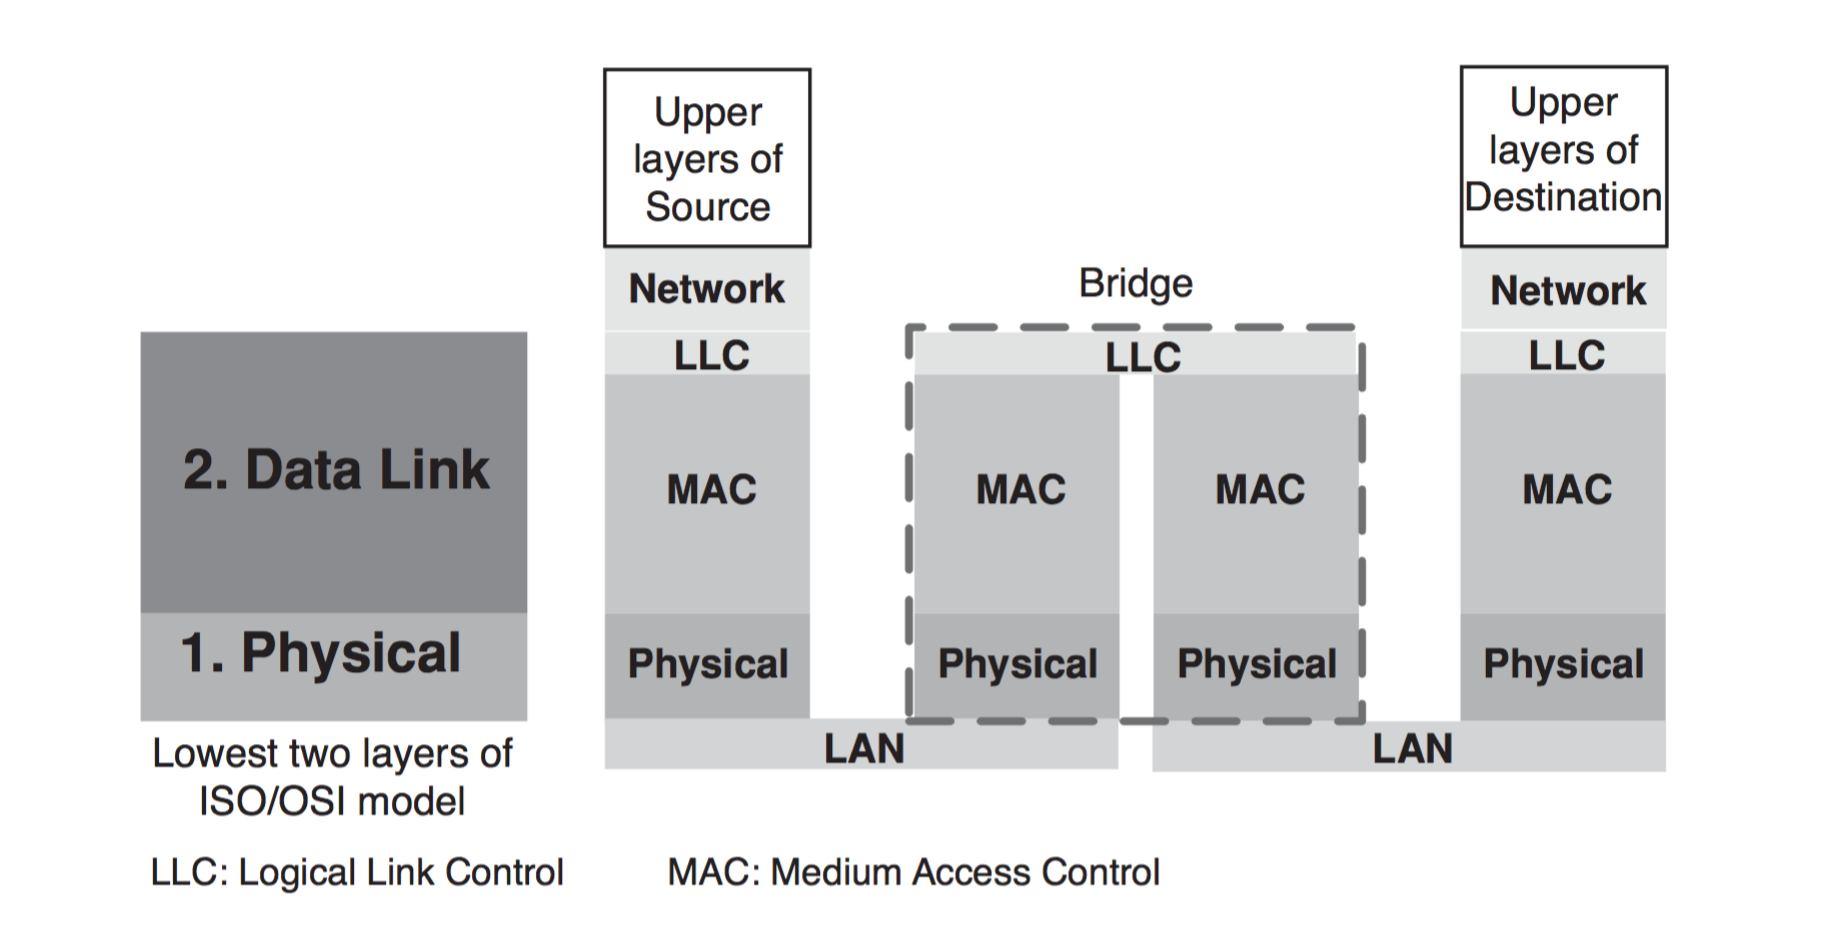
\includegraphics[scale=0.330]{imgs/arch_ieee802.png}
	\caption{Architettura IEEE 802} \label{fig:arch_802}
\end{figure}
Nella Figura in esame è mostrata la connessione di due LAN attraverso l'utilizzo di un Bridge. Tale connessione è comune in molte organizzazioni che hanno più LAN. Un pacchetto dalla sorgente va nel sottostrato Logical Link Control (LLC) che funge da interfaccia tra il livello di rete e il sottostrato MAC. LLC è definito da IEEE 802.2 e fornisce i meccanismi di controllo del flusso, multiplexing e di controllo degli errori. Il pacchetto passa poi nel sottostrato MAC in cui un header ed un trailer vengono aggiunti al pacchetto (a seconda della LAN cui il pacchetto entra). Poi si passa attraverso il livello fisico e nel canale di comunicazione e si raggiunge il Bridge. A livello MAC del Bridge, sono rimossi header e trailer, recuperando così il pacchetto originale che passa al sottostrato LLC del Bridge. Successivamente il pacchetto viene elaborato dal sottostrato MAC (aggiungendo header e trailer appropriati) in base alla LAN a cui si trasmette. L'utilizzo del Bridge è essenziale in quanto LAN diverse utilizzano differenze dimensioni del frame e velocità (e.g. IEEE 802.3 utilizza un frame di 1500 byte, mentre IEEE 802.4 ne utilizza uno di 8191 byte\cite{802.3}).
\subsubsection{Ethernet}
Ethernet è diventata la tecnologia di rete più utilizzata per le LAN cablate grazie alla sua semplicità, affidabilità, facilità di manutenzione e la capacità di integrare nuove tecnologie. Essa ha un basso costo di installazione ed è facile farne l'upgrade. Si tratta di una tecnologia di comunicazione frame-based che si basa sullo standard IEEE 802.3. Ethernet utilizza un mezzo condiviso che può portare a collisioni tra i frame trasmessi dai vari host. Il problema delle collisioni è gestito da un protocollo chiamato Carrier Sense Multiple Access/Collision Detect (CSMA/CD). Un set di host connessi ad una rete in modo tale che la trasmissione simultanea da due host nel set porta a collisioni, crea un \emph{dominio di collisione}. Inoltre, le LAN Ethernet trasportano anche frame di broadcast il cui dominio raggiungibile è denominato \emph{dominio di broadcast}. Le prestazioni della rete, in caso di traffico, sono influenzate dal modo in cui i domini di collisione e di broadcast sono posizionati e quindi l'idea è quella di isolarli per aumentare le prestazioni della rete. La Figura \ref{fig:lan} mostra tali domini su una tipica LAN Ethernet.\newpage
\begin{figure}[h]
	\centering
	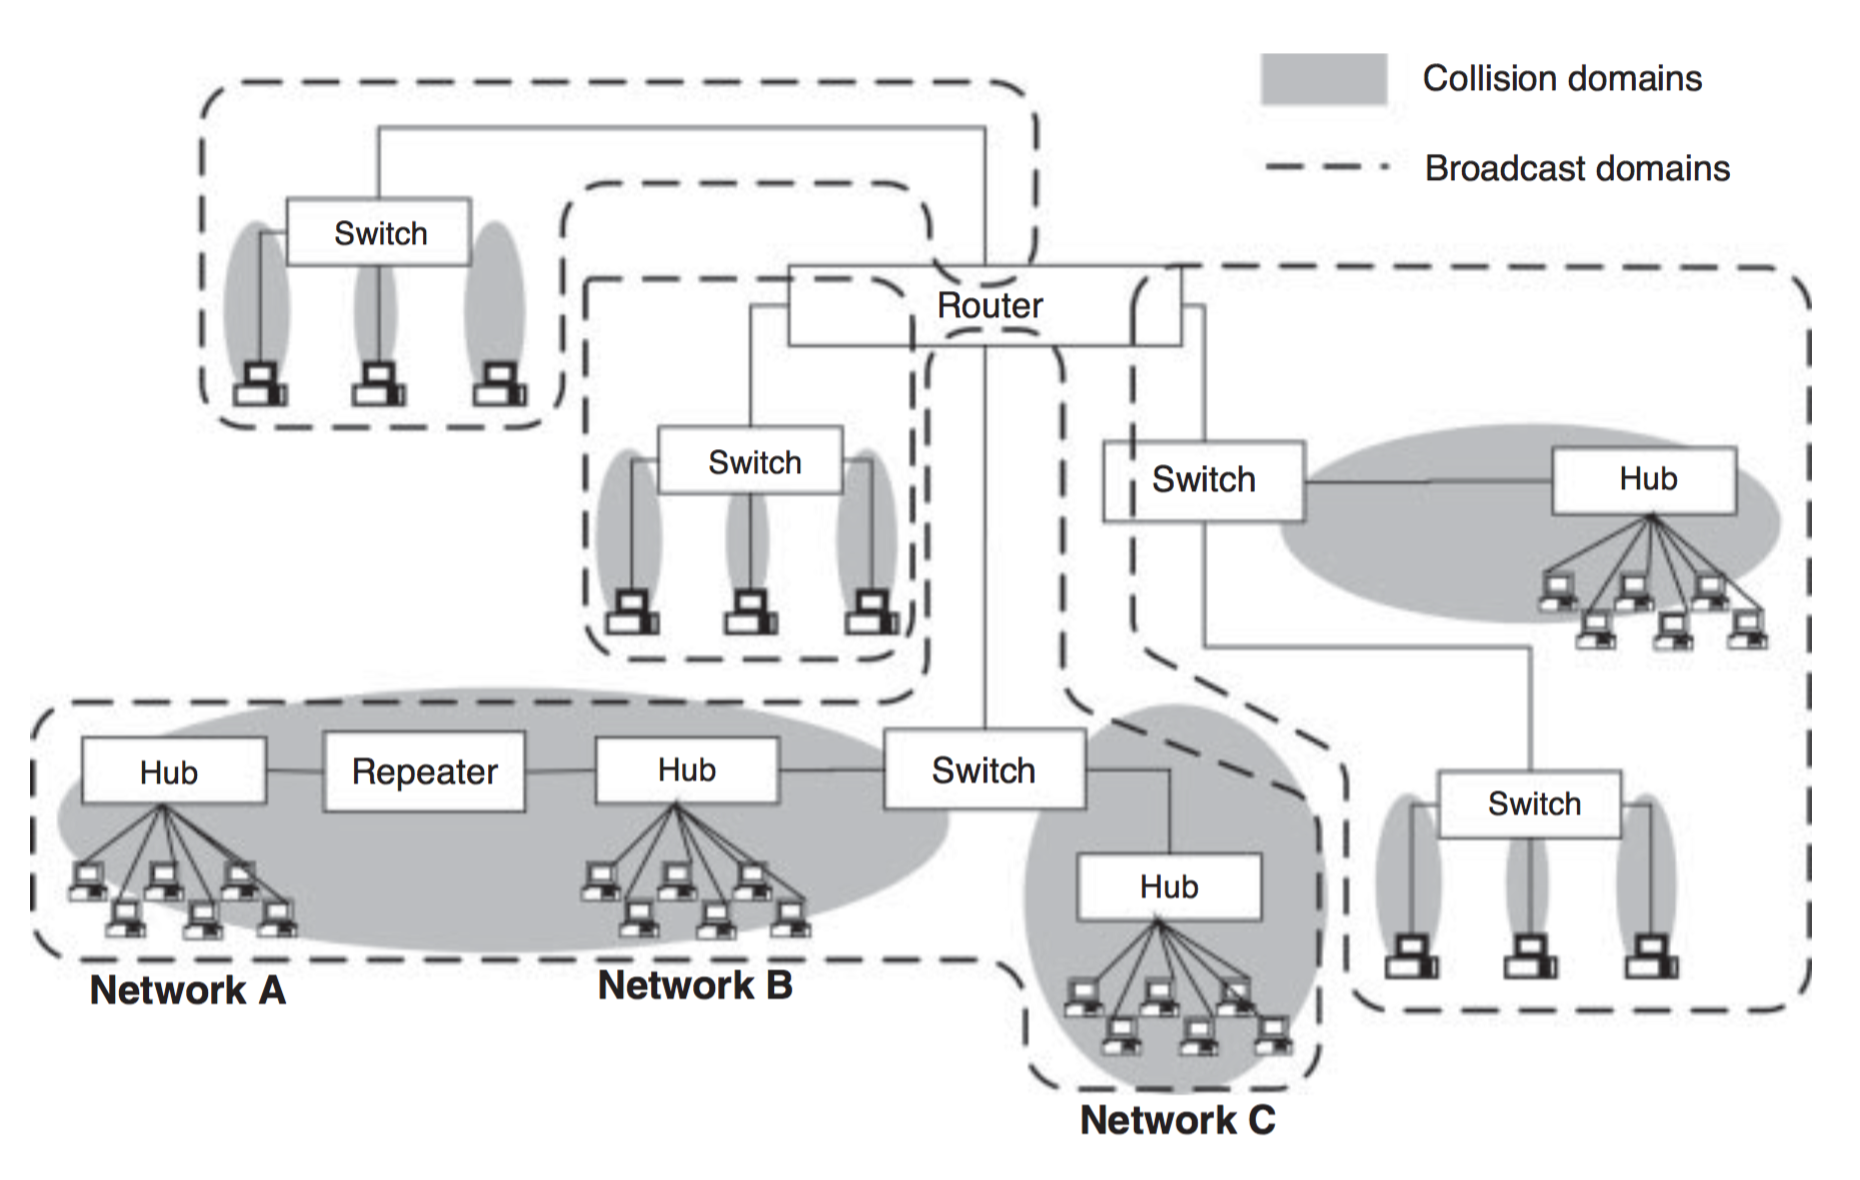
\includegraphics[scale=0.340]{imgs/lan.png}
	\caption{LAN Ethernet} \label{fig:lan}
\end{figure}
I Bridge limitano i domini di collisione mentre i Router limitano entrambi i domini. In Figura \ref{fig:lan} è mostrato come un pacchetto inviato dalla rete A può collidere con uno della rete B, ma non con uno inviato da C. Questo accade perchè vi è uno switch che limita i domini di collisione.
\subsubsection{Wireless}
IEEE 802.11 definisce un insieme di standard per le Wireless LAN (WLAN). L'interoperabilità dei dispositivi IEEE 802.11 è certificata dalla Wi-Fi Alliance. Una LAN Wireless è costituita dai seguenti componenti:
\begin{itemize}
	\item\emph{Station}: descrive qualsiasi dispositivo che comunica tramite una rete WLAN, ad esempio, un computer portatile, o cellulari che supportano WiFi. Nelle reti Ad-hoc questi dispositivi possono comunicare tra loro, creando una rete mesh (vedi Figura \ref{fig:bss}a). L'insieme di station che formano la rete Ad-hoc è chiamato Independent Basic Service Set (IBSS);
	\item\emph{Access Point (AP)}: consente ad una stazione di comunicare con un altra facendo da tramite. Necessita il doppio della larghezza di banda necessaria se la stessa comunicazione avvenisse direttamente tra le stazioni comunicanti. Gli AP rendono il sistema scalabile e consentono la connessione cablata con altre reti. In presenza di AP (vedi Figura \ref{fig:bss}b) l'insieme delle station è chiamato Infrastructure BSS;
	\item\emph{Distribution System}: interconnette Infrastructure BSS attraverso gli AP, come mostrato nella Figura \ref{fig:ds}. Facilita la comunicazione tra gli AP, l'inoltro del traffico da un BSS ad un altro ed il movimento di mobile station tra BSS. Un insieme di Infrastructure BSS è chiamato Extended Service Set (ESS).
\end{itemize}
La famiglia di reti LAN Wireless 802.11 utilizza il protocollo CSMA/CA per l'accesso al mezzo trasmissivo. Sono noti vari standard identificati da 802.11a/b/g/n/ac con variazioni a livello fisico. Una tipica applicazione di 802.11 nelle Smart Grid è mostrata in Figura \ref{fig:802_sg}.
\vspace{20pt}
\begin{figure}[h]
	\centering
	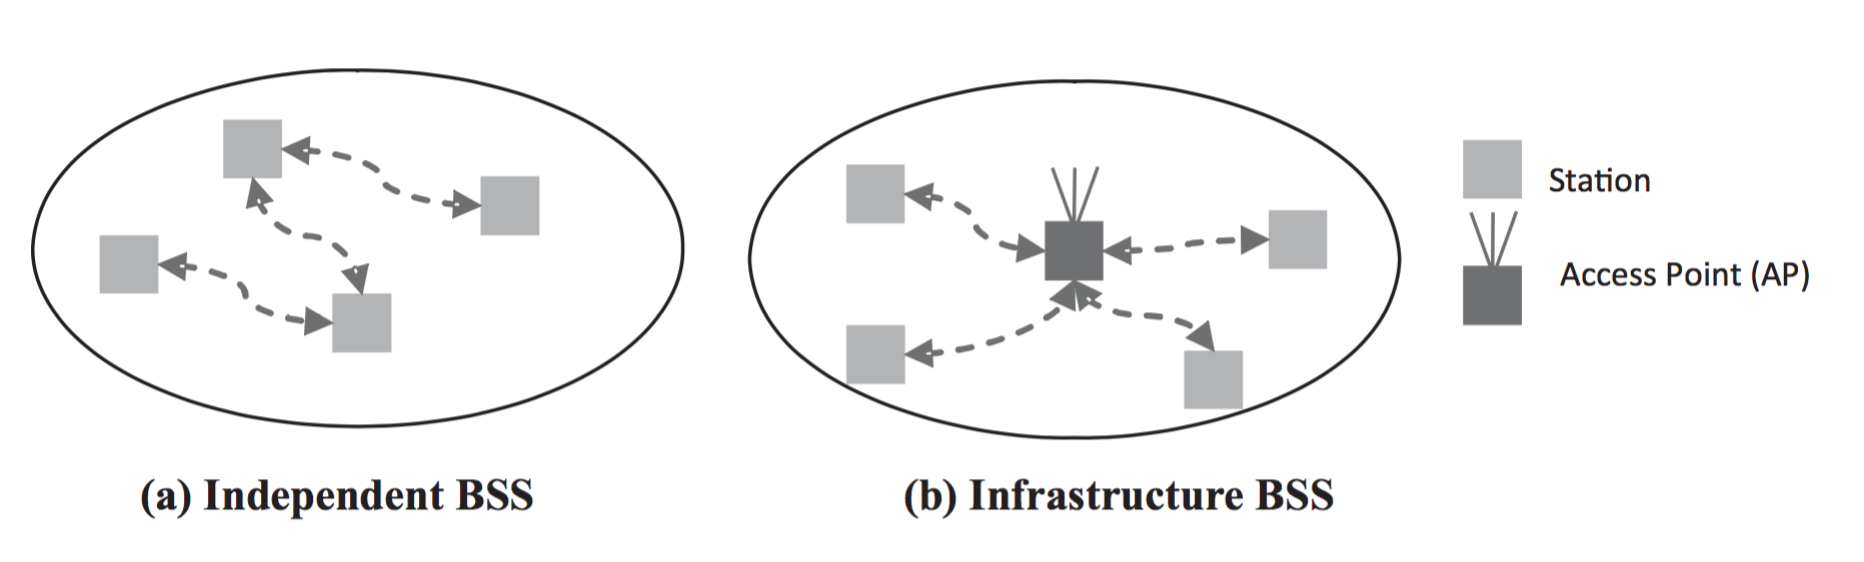
\includegraphics[scale=0.250]{imgs/bss.png}
	\caption{Architetture BSS di WLAN} \label{fig:bss}
\end{figure}
\vspace{30pt}
\begin{figure}[h]
	\centering
	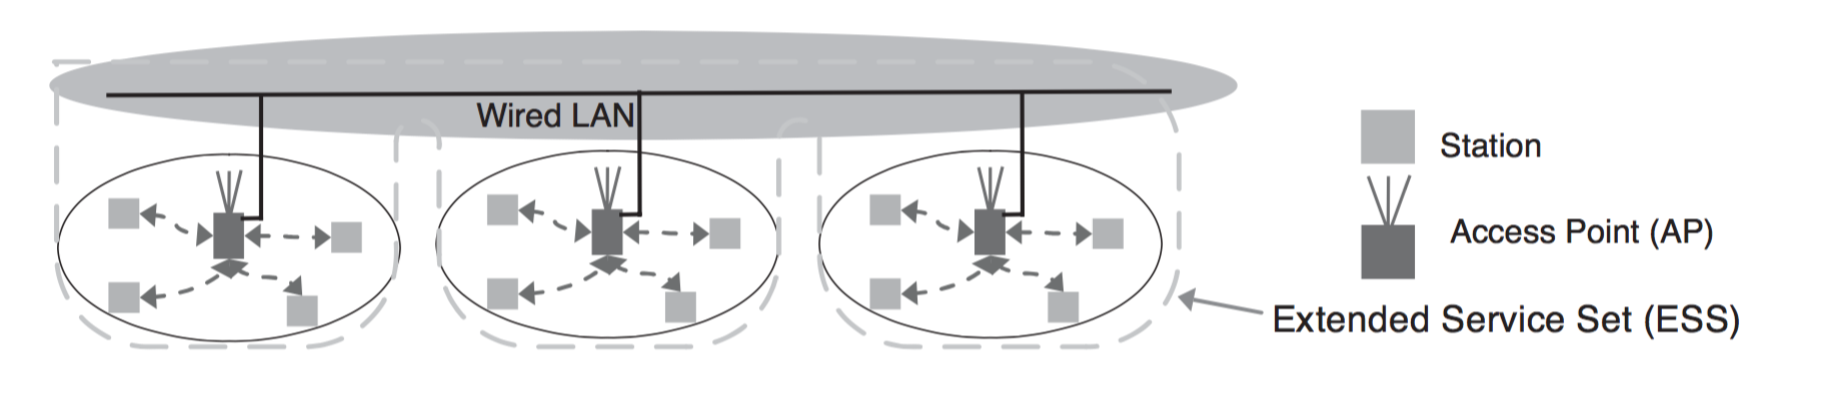
\includegraphics[scale=0.450]{imgs/ds.png}
	\caption{Distribution System} \label{fig:ds}
\end{figure}
\begin{figure}[h]
	\centering
	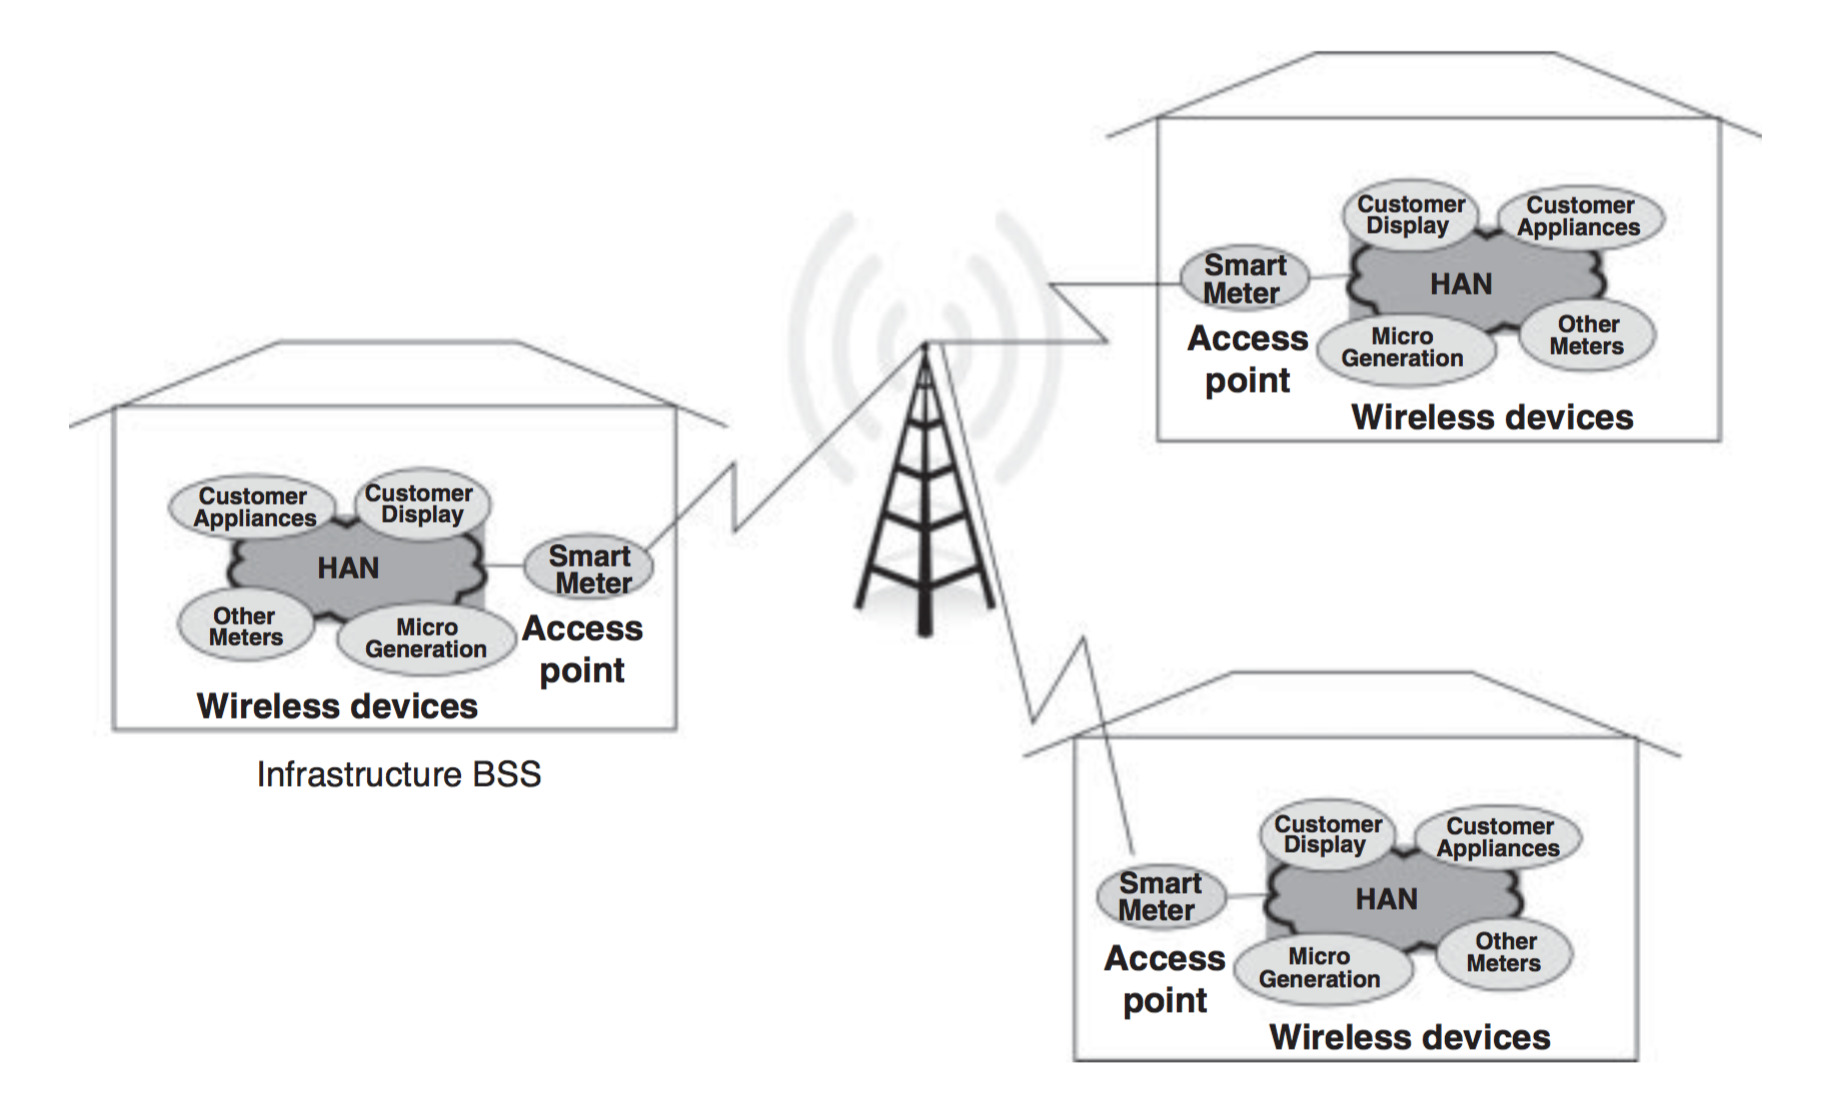
\includegraphics[scale=0.350]{imgs/80211smartgrid.png}
	\caption{Applicazione di WLAN 802.11 in una Smart Grid} \label{fig:802_sg}
\end{figure}\newpage
\subsubsection{Bluetooth}
Bluetooth, definito dallo standard IEEE 802.15.1, è una tecnologia LAN wireless progettata per collegare i dispositivi mobili o fissi con bassi consumi, un corto raggio d'azione (fino a 100 metri di copertura per un dispositivo di Classe 1 e fino ad un metro per dispositivi di Classe 3) e un basso costo di produzione per i dispositivi compatibili. 
Bluetooth definisce due architetture di rete denominate Piconet e Scatternet. La Piconet è costituita da un dispositivo \emph{Master} e fino a sette dispositivi \emph{Slave}. Altri dispositivi possono sincronizzarsi col Master ma non possono partecipare alla comunicazione. Si dice che tali dispositivi sono in un parked state. Un device in parked state può passare in active state se il numero di Slave della Piconet è inferiore a sette. Le Piconet possono essere interconnesse attraverso un Bridge che può essere Slave per una Piconet e Master per un'altra oppure Slave per due Piconet che sono interconnesse come in Figura \ref{fig:bt}a e \ref{fig:bt}b. Un insieme di Piconet forma una Scatternet.\newpage
Per il trasferimento dei dati è possibile creare due tipi di collegamenti bluetooth:
\begin{itemize}
		\item Synchronous Connection Orientated (SCO) link
		\item Asynchronous Connectionless Link (ACL)
\end{itemize}
SCO è utilizzato quando la consegna tempestiva è più importante della consegna senza errori mentre ACL è utilizzato nel caso inverso.
\begin{figure}[h]
	\centering
	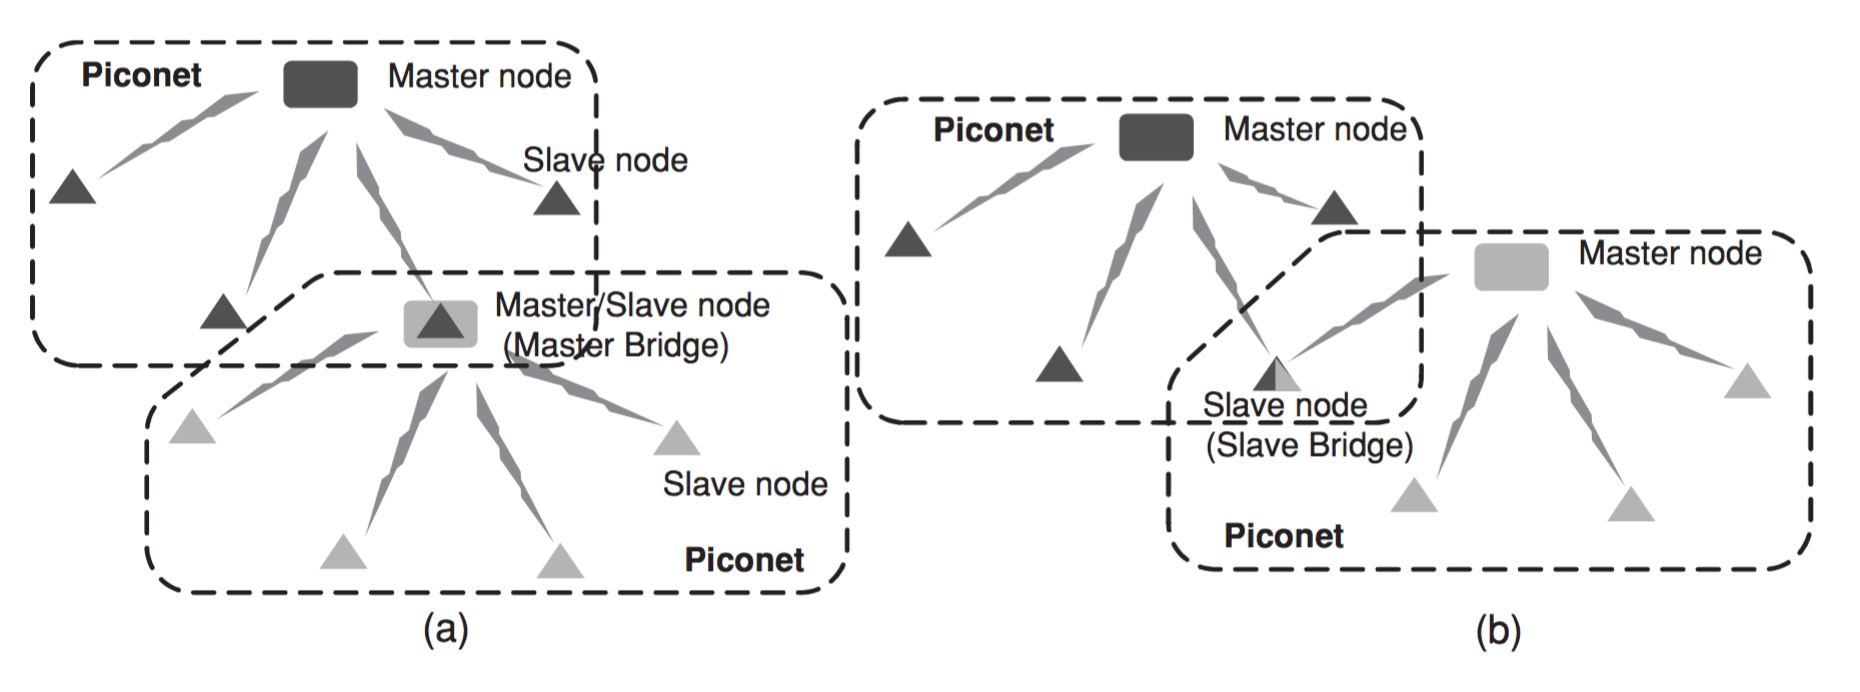
\includegraphics[scale=0.350]{imgs/bt.png}
	\caption{Piconet e Scatternet} \label{fig:bt}
\end{figure}
\subsubsection{ZigBee and 6LoWPAN}
ZigBee e 6LoWPAN sono due tecnologie di comunicazione basate su IEEE 802.15.4 per Wireless Personal Area Network (WPAN) dato il basso consumo, l'alta flessibilità ed i basso costi. L'architettura protocollare di un device ZigBee è mostrata nella Figura \ref{fig:zbprot} in cui i due strati inferiori sono definiti da IEEE 802.15.4. Application Support e Network Layer per la rete ZigBee sono definiti dalla ZigBee Alliance\cite{zb}.
\begin{figure}[h]
	\centering
	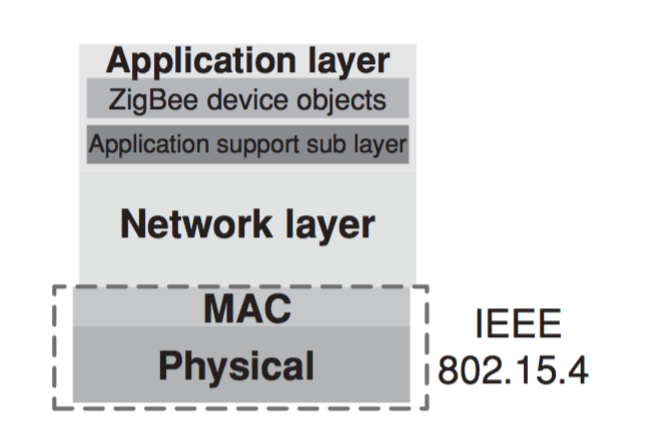
\includegraphics[scale=0.400]{imgs/zbprot.png}
	\caption{Architettura Protocollare di ZigBee} \label{fig:zbprot}
\end{figure}\newpage
Un device ZigBee può essere un Full Function Device (FFD) o un Reduced Function Device (RFD). Una rete avrà almeno un FFD, che fungerà da coordinatore della WPAN. Il FFD può funzionare in tre modalità: coordinatore, router o device. Un RFD può funzionare solo come device. Un FFD può interagire sia con un altro FFD che con un RFD, mentre un RFD può parlare solo con un FFD.
La tecnologia ZigBee è considerata come una buona opzione per il metering e per la gestione dell'energia ideale in implementazioni Smart Grid data la semplicità, mobilità, robustezza e i bassi costi di sviluppo. Offre anche programmi di pricing e monitoraggio del sistema real-time. ZigBee presenta però alcuni vincoli relativi alle basse capacità di elaborazione, alla piccola dimensione della memoria e alle interferenze tra i vari apparecchi che condividono lo stesso mezzo trasmissivo. Tali problematiche, in condizioni di rumore, aumentano la possibilità di danneggiare il canale di comunicazione a causa delle interferenze. Schemi di interference detection/avoidance e protocolli di routing energy-efficient estendono il tempo di vita della rete e forniscono una performance di rete affidabile e ad alta efficienza dal punto di vista energetico.
\newline\newline
6LoWPAN è un protocollo che consente l'invio e la ricezione di pacchetti IPv6 nelle reti basate su IEEE 802.15.4. In tale protocollo è stato inserito un Adaptation Layer (vedi Figura \ref{fig:6pan}) per il collegamento tra lo strato MAC e il Network Layer IPv6.
%Il concetto 6LoWPAN nasce dall'idea che "il protocollo Internet potrebbe e dovrebbe essere applicato anche ai dispositivi più piccoli, e che i dispositivi a bassa potenza e con capacità di elaborazione limitate dovrebbero essere in grado di far parte dell' Internet of Things".
\begin{figure}[h]
	\centering
	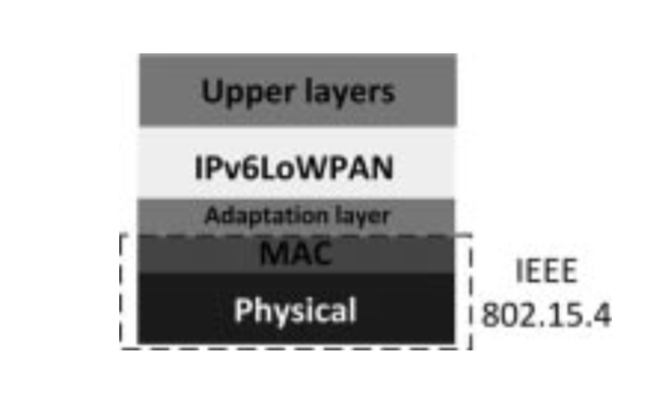
\includegraphics[scale=0.400]{imgs/6pan.png}
	\caption{Architettura di rete 6LoWPAN} \label{fig:6pan}
\end{figure}
\\
Quando un RFD in una 6LoWPAN vuole inviare un pacchetto di dati ad un dispositivo che si trova al di fuori del dominio 6LoWPAN, invia inizialmente il pacchetto ad un FFD nella stessa WPAN. Il FFD che agisce da router, inoltrerà il pacchetto dati di hop in hop fino al gateway 6LoWPAN. Il gateway 6LoWPAN potrà quindi inoltrare il pacchetto al dispositivo di destinazione utilizzando l'indirizzo IP (vedi Figura \ref{fig:6pancom}).
\begin{figure}[h]
	\centering
	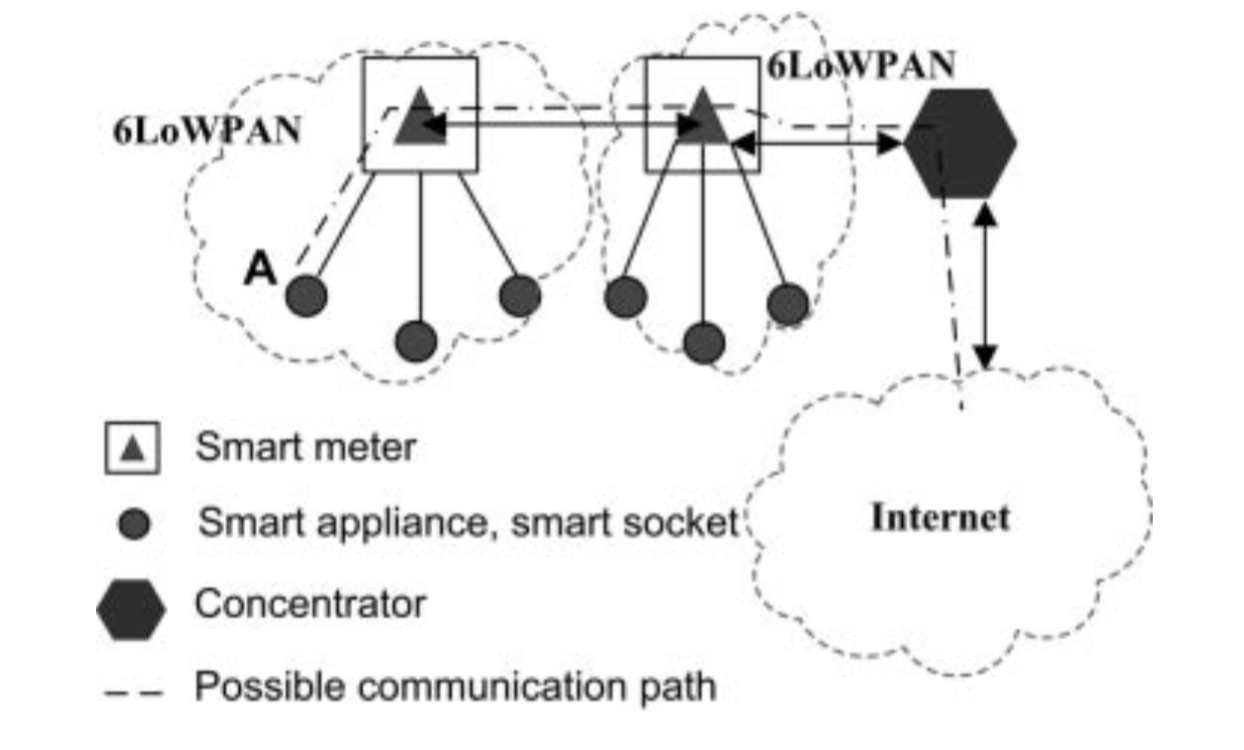
\includegraphics[scale=0.450]{imgs/6pancom.png}
	\caption{Comunicazione in una rete 6LoWPAN} \label{fig:6pancom}
\end{figure}
\subsubsection{WiMax}
Worldwide Interoperability for Microwave Access (WiMAX) è una tecnologia wireless conforme allo standard IEEE 802.16. Risulta superiore rispetto a Wi-Fi per velocità di trasmissione e range di copertura delle celle, per cui è adatto ad una trasmissione sia di tipo urbano che rurale. Inoltre, implementa diverse tecniche di crittografia, sicurezza ed autenticazione. WiMAX è una tecnologia in grado di integrarsi con quelle presenti, soddisfacendo diverse specifiche imposte da una tipica Smart Grid tra cui la massima accessibilità ed interoperabilità, tempi di latenza inferiori ai 50ms e larghezza di banda di 5MHz. Fornisce sia connettività fissa che mobile usando una tecnica chiamata Orthogonal Frequency Division Multiple Access (OFDMA). Una tipica rete WiMax è mostrata in Figura \ref{fig:wim}. La copertura di WiMax si estende fino ai 50 km con una velocità di trasmissione dati pari a 75 Mbps per i collegamenti fissi e fino a 15 Mbps per le connessioni mobili. È ottimizzato per supportare dispositivi mobili fino ad una velocità di 10 km/h. Anche se supporta veicoli in movimento fino a 120 km/h, le sue prestazioni degradano con l'aumentare della velocità del veicolo\cite{wimax}.
\begin{figure}[h]
	\centering
	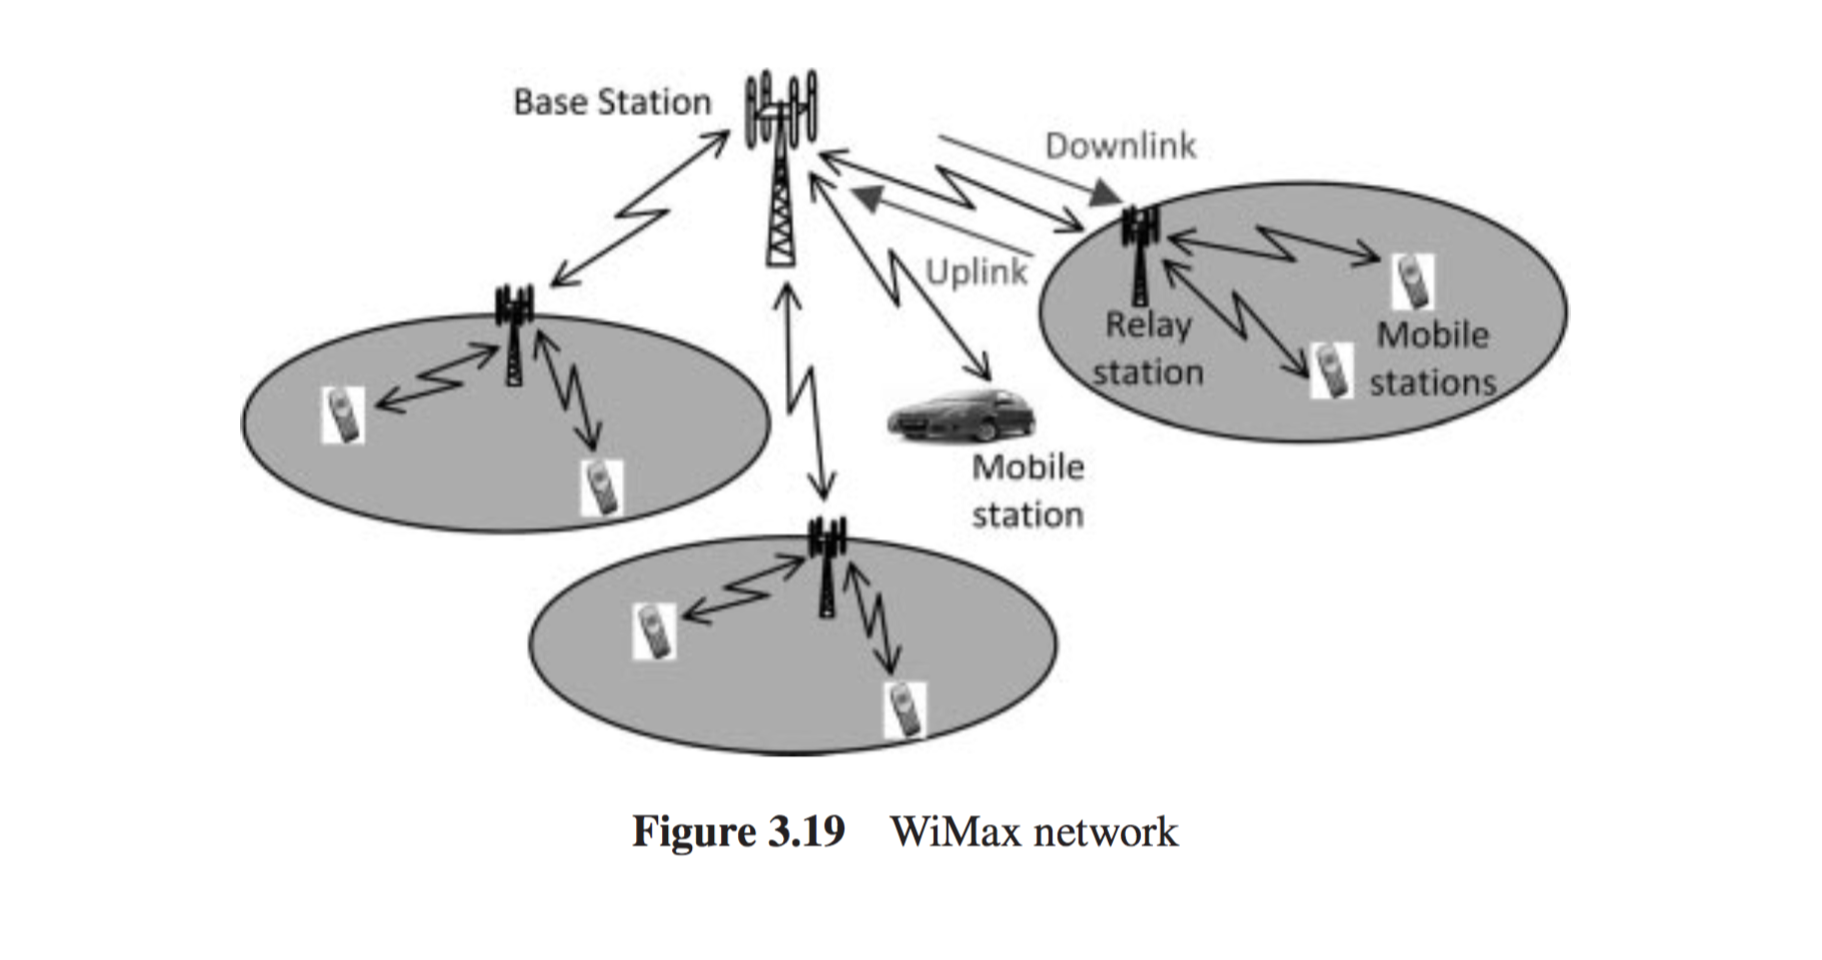
\includegraphics[scale=0.350]{imgs/wim.png}
	\caption{Una rete WiMax} \label{fig:wim}
\end{figure}
\newpage
\subsection{Power line}
La Power Line Communication (PLC) rappresenta una delle tecnologie di rete proposte per la trasmissione in ambiente Smart Grid in quanto l'infrastruttura esistente riduce i costi di installazione di un'ulteriore infrastruttura di comunicazione. Se, da un lato non è richiesta la realizzazione di nuove strutture, da un altro lato vi è un limite dovuto alla presenza di disturbi che possono corrompere le informazioni, non garantendo più la continuità del servizio. PLC trasporta i dati utilizzando i conduttori e le linee elettriche esistenti. Fornisce servizi di comunicazione per Automatic Meter Reading (AMR), AMI e HAN ma anche l'accesso ad internet all'utente finale. In una tipica rete PLC, gli smart meter sono collegati al data concentrator (che colleziona le informazioni ricevute dai vari meter) attraverso power line e i dati vengono trasferiti al data center tramite tecnologie di rete cellulare. La tecnologia PLC è infatti scelta per la comunicazione tra gli smart meter e il data concentrator, mentre la tecnologia GPRS è utilizzata per trasferire i dati dal concentrator al data center.\newline\newline
L'ENEL, nota azienda multinazionale produttrice e distributrice di energia elettrica, ha scelto la tecnologia PLC per trasferire i dati degli smart meter al data concentrator più vicino e la tecnologia GSM per inviare i dati al data center.
La topologia di rete, il numero/tipo dei dispositivi collegati e la distanza trasmettitore/ricevitore compromettono la qualità del segnale.
\newpage
La sensibilità di PLC ai disturbi e la dipendenza alla qualità segnale sono gli svantaggi che rendono la tecnologia non adatta alla trasmissione dei dati. Tuttavia, ci sono state alcune soluzioni ibride in cui la tecnologia PLC si combina con altre, ad esempio, GPRS o GSM, per fornire una connettività non possibile generalmente con PLC.\newline\newline
Inizialmente, la velocità di trasmissione in questo tipo di reti era molto limitata, fino a pochi kbps. Successivamente, grazie al progresso tecnologico e con l'introduzione di broadband PLC (BB-PLC), un'applicazione della tecnologia PLC a banda larga che fornisce l'accesso a Internet tramite linee elettriche ordinarie, la velocità di trasmissione ha raggiunto anche i 200 Mbps. Tre sono le diverse tecnologie di comunicazione utilizzate, vale a dire, \emph{narrowband transmission}, \emph{spread-spectrum transmission} e \emph{DSP-processed narrowband transmission}. La Figura \ref{fig:vs_plc} mostra alcuni vantaggi e svantaggi relativi a PLC in ambito Smart Grid. Tra gli standard e i protocolli maggiormente utilizzati troviamo IEEE P1901 e HomePlug.\vspace{20pt}
\begin{figure}[h]
	\centering
	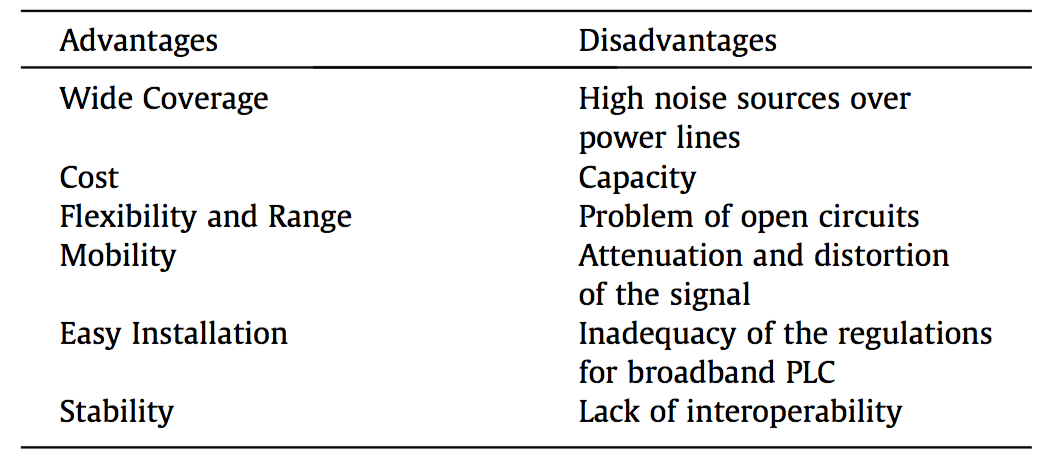
\includegraphics[scale=0.500]{imgs/vs_plc.png}
	\caption{Vantaggi e Svantaggi di PLC in ambito Smart Grid} \label{fig:vs_plc}
\end{figure}
\newpage
\subsubsection{IEEE P1901}
Il gruppo IEEE P1901 è stato formato nel 2005 con lo scopo di sviluppare una tecnologia per la trasmissione di voce o dati che utilizzasse la rete di alimentazione elettrica come mezzo trasmissivo. Lo standard permette una comunicazione ad altà velocità tra i device che prendono il nome di BPL (Broadband over Power Line). Lo standard utilizza frequenze inferiori a 100 MHz ed è di supporto ai device BPL utilizzati per i collegamenti first-mile/last-mile così come quelli utilizzati nelle reti LAN all'interno di edifici. Inoltre, tali device possono essere utilizzati all'interno di smart energy application, autoveicoli e in altre applicazioni per la distribuzione dei dati.
\subsubsection{HomePlug}
HomePlug è una tecnologia broadband non standardizzata e specificata dalla HomePlug Powerline Alliance, i cui membri sono le principali aziende nel settore della comunicazione e dell'energia. Il protocollo gestisce vari sottocanali suddividendo la larghezza di banda disponibile. La velocità di trasmissione varia da 1 a 14 Mbps e i nodi sono in grado di adattarsi al data rate ottimale in maniera automatica. Le collisioni sono evitate grazie al CSMA/CD. Lo standard HomePlug 1.0 per la connessione di dispositivi nelle case (1-10 Mbps) fa uso della tecnica di Orthogonal Frequency Division (OFDM), utilizzata anche da DSL, IEEE 802.11a e IEEE 802.11g. Il rumore, comune in ambiente power line, è superato per mezzo di forward error correction e data interleaving. La HomePlug Powerline Alliance ha definito ulteriori standard come HomePlug AV/AV2 che forniscono banda sufficiente per applicazioni come HDTV e VoIP, HomePlug CC e HomePlug BPL.
\section{Standard per lo scambio di informazioni}
\subsubsection{Standard per Smart Meter}
Gli smart meter possono essere utilizzati in vari modi portando a differenti requisiti dal punto di vista del sistema di comunicazione. Con Automated Meter Reading (AMR) si richiede una trasmissione occasionale dei dati energetici registrati (circa una volta al mese), viceversa con  Advanced Metering Infrastructure (AMI) si richiedono frequenti comunicazioni bidirezionali (ad esempio ogni 30 minuti). IEC 62056 e ANSI C12.22 sono due famiglie di standard che descrivono sistemi di comunicazione per gli smart meter. IEC 62056 definisce Transport e Application Layer per lo smart metering nell'ambito di una serie di specifiche chiamate COSEM (Companion Specification for Energy Metering). ANSI C12.22 (vedi Figura \ref{fig:arch_c1222}) specifica l'invio e la ricezione dei dati registrati da e verso sistemi esterni ed è possibile utilizzarlo su qualsiasi rete di comunicazione.
\begin{figure}[h]
	\centering
	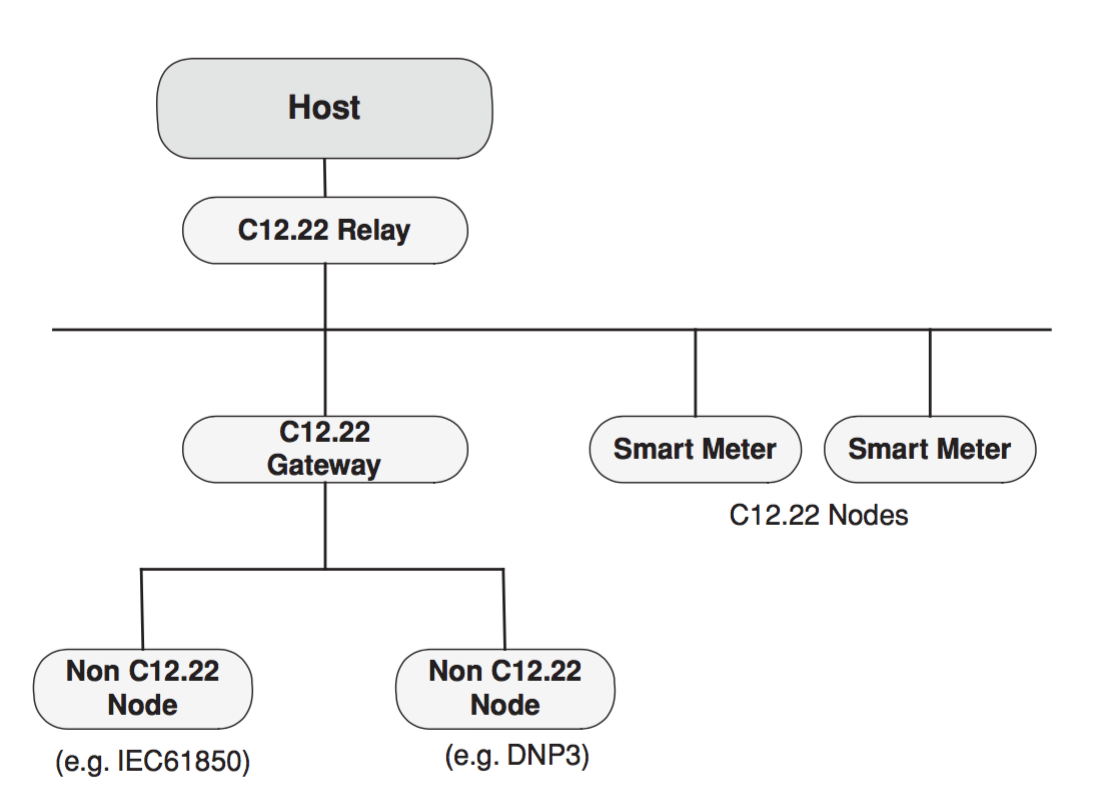
\includegraphics[scale=0.400]{imgs/arch_c1222.png}
	\caption{Architettura ANSI C12.22} \label{fig:arch_c1222}
\end{figure}
\subsubsection{Modbus}
Modbus è un protocollo di messaggistica che risiede nell'Application Layer e consente la comunicazione tra i dispositivi collegati su diversi bus e reti. Può essere implementato tramite Ethernet o utilizzando la trasmissione seriale asincrona su EIA 232, EIA 422, EIA 485 e fibra ottica. Di questi, l'applicazione più comune è Modbus su EIA485. La Figura \ref{fig:modbus} mostra come l'Application Layer Modbus è connesso agli altri layer del modello OSI.
Modbus su EIA 485 è ampiamente utilizzato nell'automazione delle sottostazioni. La comunicazione è avviata dal Master con una query. Il Master è l'unico che può inviare query destinate al singolo Slave o di broadcast. Uno Slave monitora continuamente la rete riconoscendo solo le query destinate ad esso. All'arrivo di una query, lo Slave eseguirà un'azione o risponderà. Tra i problemi del protocollo spiccano il limitato supporto alle varie tipologie di dati e la non garanzia di sicurezza.
\begin{figure}[h]
	\centering
	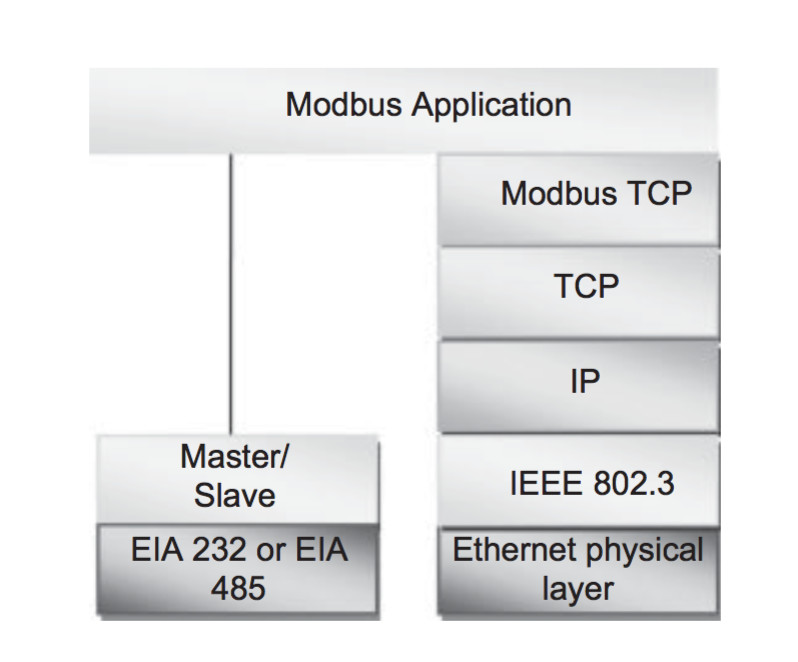
\includegraphics[scale=0.500]{imgs/modbus.png}
	\caption{Modbus stack} \label{fig:modbus}
\end{figure}
\newpage
\subsubsection{DNP3}
DNP3 è un insieme di protocolli di comunicazione utilizzato tra i componenti nei sistemi di automazione. DNP3 gioca un ruolo fondamentale all'interno dei sistemi SCADA, utilizzato dalle SCADA Master Station (conosciute anche come \emph{centri di controllo}) per comunicare con le Remote Terminal Unit (RTU) e/o gli Intelligent Electronic Device (IED). DNP3 è stato recentemente adottato come standard IEEE 1815-2010\cite{dnp}. Lo User Layer DNP prende input analogici/binari e da in output segnali analogici/binari. Un Master DNP3 invia richieste e le stazioni Slave DNP3 rispondono. Uno Slave DNP3 può anche trasmettere un messaggio senza aver ricevuto alcuna richiesta. Il Physical Layer DNP3 utilizza alcuni tra i più noti protocolli di comunicazione seriali come EIA 232 o EIA 485.
\newline\newline
Poiché nelle applicazioni di tipo Smart Grid generalmente si presume l'accesso di terze parti alla stessa rete e all'infrastruttura sottostante basata su protocollo IP, un passo in avanti è stato quello che ha portato all'aggiunta di un'autenticazione sicura al protocollo DNP3. Alcuni vendors supportano la crittografia via \textbf{bump-in-the-wire} (cioè con dispositivi esterni che cifrano/decifrano i dati agli estremi del canale di comunicazione) per le comunicazioni seriali e tramite VPN per le reti IP. Uno dei metodi bump-in-the-wire più popolari era noto come \emph{AGA-12} (American Gas Association).
\subsubsection{IEC 61850}
IEC 61850 è uno standard per la progettazione dei sistemi di automazione per le sottostazioni elettriche. E' una sovrastruttura che coordina e gestisce protocolli e tecnologie esistenti garantendo l'interoperabilità. Generalmente, questi protocolli girano su reti TCP/IP o LAN con switch Ethernet molto performanti per rispondere ai requisiti stringenti dei dispositivi, che necessitano di tempi di risposta inferiori a 4-5 millisecondi.\newline\newline
I principali vantaggi dello standard IEC 61850:
\begin{itemize}
	\item Coordina la complessità di tante unità indipendenti;
	\item Si integra con i sistemi preinstallati in rete;
	\item E' scalabile e facilita l'integrazione di apparati diversi;
	\item Si basa il più possibile su standard esistenti;
	\item E' aperto e supporta i \emph{self descriptive device} eliminando problemi di configurazione manuale;
	\item Si basa sui \emph{data object} e standardizzazione degli elementi tipici di una rete elettrica;
	\item Permette di ottenere alte prestazioni di multicast;
	\item E' estensibile e flessibile in modo da adattarsi rapidamente alla configurazione del sistema.
\end{itemize}
\newpage
La struttura dello standard IEC 61850\cite{iec61850} è mostrata in Figura \ref{fig:iec61850}.
\begin{figure}[h]
	\centering
	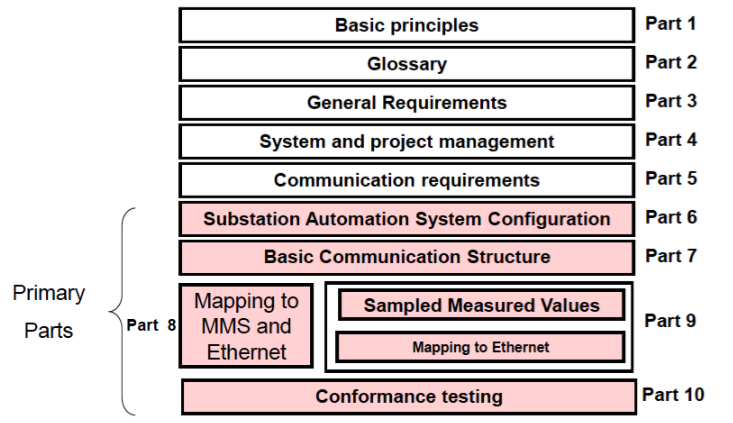
\includegraphics[scale=0.400]{imgs/iec61850.png}
	\caption{Struttura dello standard IEC 61850} \label{fig:iec61850}
\end{figure}\\
IEC 61850 suddivide ogni sottostazione in tre livelli\cite{iec61850} chiamati Station Level, Bay Level e Process Level. La suddivisione dei livelli è mostrata in Figura \ref{fig:61850ls}.

\begin{figure}[h]%si potrebbe omettere
	\centering
	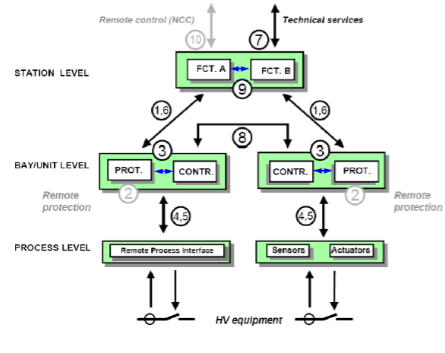
\includegraphics[scale=0.400]{imgs/61850ls.png}
	\caption{Livelli di una sottostazione} \label{fig:61850ls}
\end{figure}

Il protocollo identifica le funzioni e le caratteristiche dei dispositivi fisici che si modellano in uno o più dispositivi logici. I dispositivi logici sono a loro volta suddivisi in nodi logici che sono in relazione tra loro in base a \emph{data} e \emph{data attribute} (vedi Figura \ref{fig:iec61850ln}).
\begin{figure}[h]
	\centering
	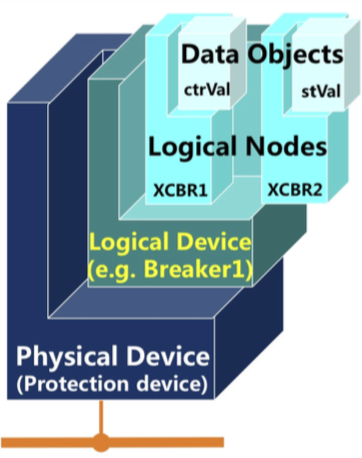
\includegraphics[scale=0.350]{imgs/iec61850ln.png}
	\caption{Device Model IEC 61850} \label{fig:iec61850ln}
\end{figure}
\newpage
Come mostrato in Figura \ref{fig:iec61850ds}a, un device model considera inizialmente un physical device. Tale modello consente ad un singolo dispositivo fisico di agire da gateway di informazioni per più dispositivi. Successivamente vengono specificati i logical device all'interno di tale dispositivo. Ogni logical device contiene uno o più logical node, logicamente correlati ad una funzione della stazione. I logical node sono definiti da gruppi di data object e relativi servizi, ognuno modellato secondo gli schemi definiti dalle \textbf{Common Data Classes} (CDC).\newline
\begin{figure}[h]
	\centering
	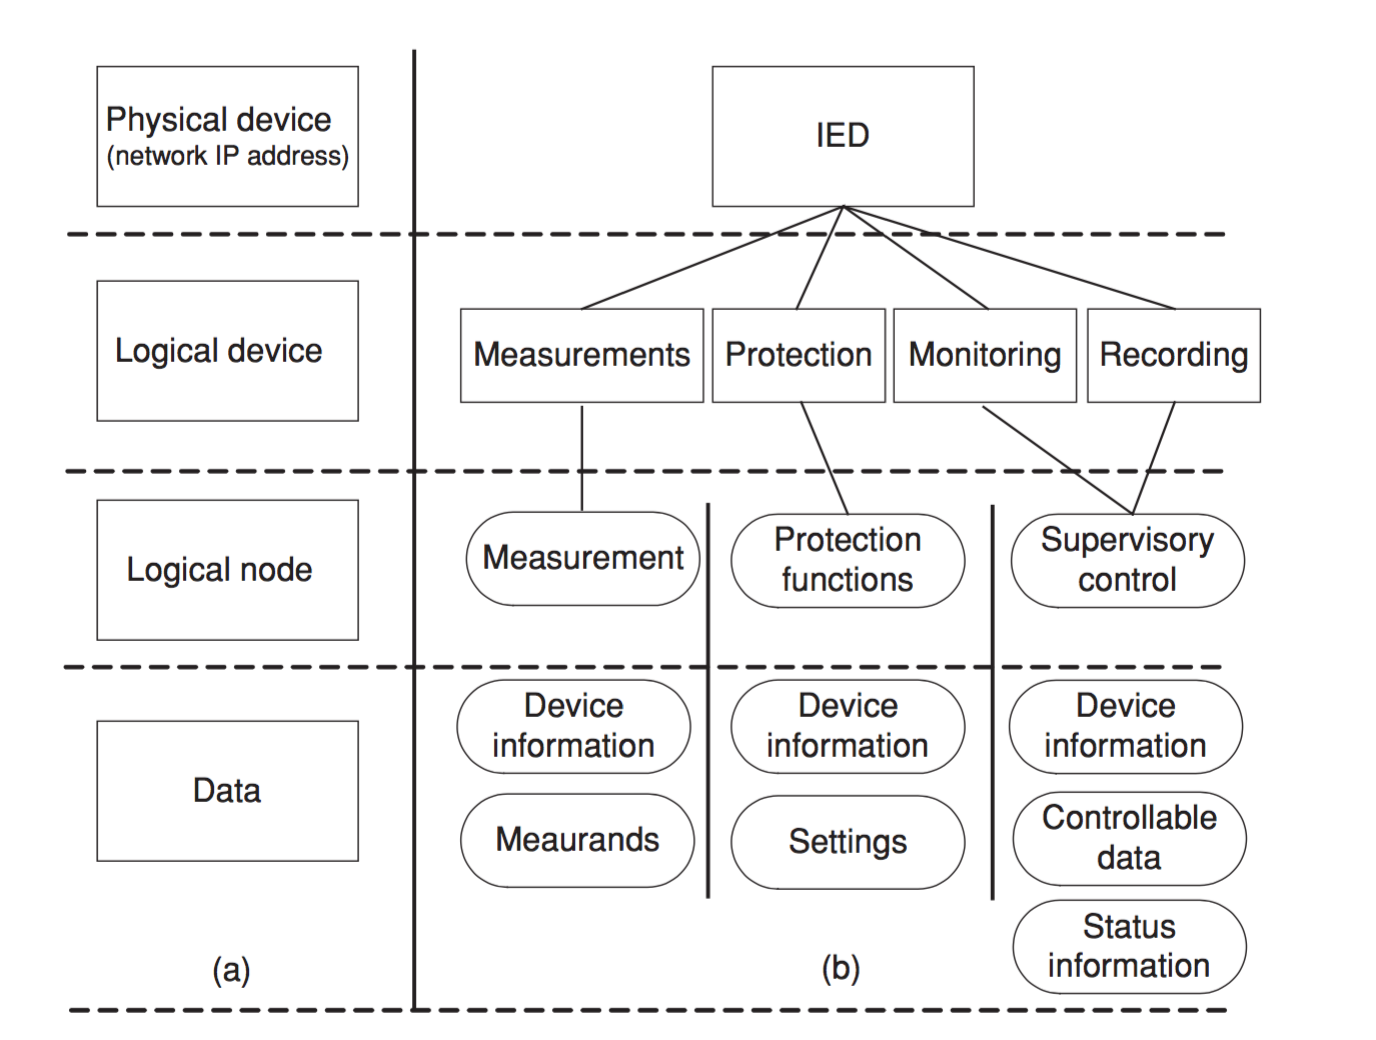
\includegraphics[scale=0.350]{imgs/iec61850ds.png}
	\caption{IEC 61850 data structure} \label{fig:iec61850ds}
\end{figure}\newpage
La Figura \ref{fig:name_obj} mostra un esempio di nome per un oggetto in un formato standard. Utilizzando tale formato si è in grado di indicare le informazioni relative allo status o alla posizione di un dispositivo. I logical node sono identificati con nomi definiti dallo standard in cui la prima lettera indica l'attinenza (e.g. A controllo automatico, M misura, X switchgear, etc).
\begin{figure}[h]
	\centering
	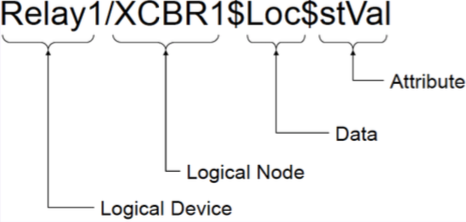
\includegraphics[scale=0.350]{imgs/name_obj.png}
	\caption{Struttura del nome di un oggetto} \label{fig:name_obj}
\end{figure}
\newline
L'IEC 61850 si basa sulla definizione di astrazione di dati e servizi specificando \emph{oggetti} e \emph{servizi astratti} di comunicazione che permettono di scrivere un'applicazione indipendentemente dai protocolli tradizionali. Si definisce quindi un modello che prende il nome di Abstract Communication Service Interface (ACSI) che definisce l'insieme dei servizi e le risposte a quei servizi che rendono gli IED uguali dal punto di vista della rete. Inoltre, tale modello interpreta i dati e gli attributi dei vari elementi garantendone l'interoperabilità. Gli oggetti e i servizi definiti dall'ACSI vengono implementati attraverso il protocollo ISO-9560 Manufacturing Message Specification (MMS). Si tratta di un protocollo flessibile in grado di supportare funzioni complesse e la logica a oggetti ACSI. Tale protocollo definisce i messaggi di comunicazione tra i vari centri di controllo oppure tra le stazioni e i centri di controllo.\newline\newline
Il concetto di astrazione e standardizzazione presuppone l'utilizzo di un linguaggio comune di configurazione. L'IEC 61850 si serve di un linguaggio basato su \emph{XML} chiamato \emph{Substation Configuration Language} (SCL). Grazie all'utilizzo di un linguaggio standard è possibile garantire l'interoperabilità tra gli IED che usano diversi protocolli, permettere una configurazione automatica dei dispositivi, ridurre la componente di errore dovuta all'intervento umano nella gestione degli IED e consentire maggiore trasportabilità facendo in modo che ogni IED, che supporta IEC 61850, presenta un file SCL che ne definisce la configurazione. Nella Figura \ref{fig:iec61850ds}b è mostrato un esempio di IED.\newpage
Gli elementi fondamentali del modello di una sottostazione sono elencati di seguito (vedi Figura \ref{fig:arch_iec61850}):
\begin{itemize}
	\item\textbf{Merge Unit}: A livello di processo, i dati raccolti da sensori ottici, elettronici, da TV e TA, sui valori di tensione e corrente o sullo status dei componenti, sono raccolti da Merge Unit (MU). In genere sono localizzate in corrispondenza del centro di controllo;
	\item\textbf{Intelligent Electronic Device}: Gli IED che supportano IEC 61850 comunicano attraverso le MU e un process bus Ethernet a 10 Gbps;
	\item\textbf{Wrapper IEC 61850}: Gli IED che non supportano il protocollo IEC 61850 utilizzano un Wrapper;
	\item\textbf{Process Bus e Station Bus}: Le MU comunicano con il Bay Level attraverso un process bus mentre tutti i nodi logici (IED) comunicano attraverso un bus Ethernet a 100 Mbps;
	\item\textbf{Gateway e Internet}: Diverse sottostazioni comunicano tra loro attraverso la rete Internet. Un Gateway permette di collegarsi alla rete e accedere alle informazioni da un centro di controllo o da remoto seguendo una procedura che garantisce la robustezza e sicurezza del sistema.
\end{itemize}

\begin{figure}[h]
	\centering
	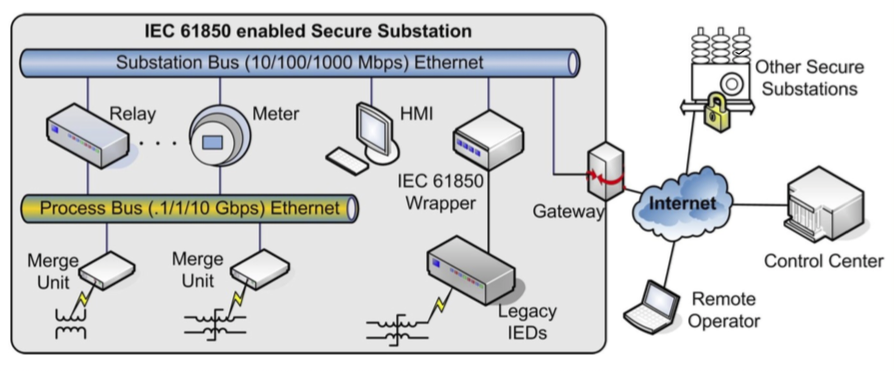
\includegraphics[scale=0.450]{imgs/arch_iec61850.png}
	\caption{Architettura del sistema con lo standard IEC 61850} \label{fig:arch_iec61850}
\end{figure}
\newpage
Lo standard IEC 61850 si serve dei seguenti strumenti per la gestione delle informazioni (vedi Figura \ref{fig:tools_iec61850}):
\begin{itemize}
	\item Generic Substation Event (GSE);
	\begin{itemize}
		\item Generic Object Oriented Substation Event (GOOSE);
		\item Generic Substation State Event (GSSE).
	\end{itemize}
	\item Sampled Measured Values (SMV);
	\item Time Synchronization;
	\item Report e Logging.
\end{itemize}
\begin{figure}[h]
	\centering
	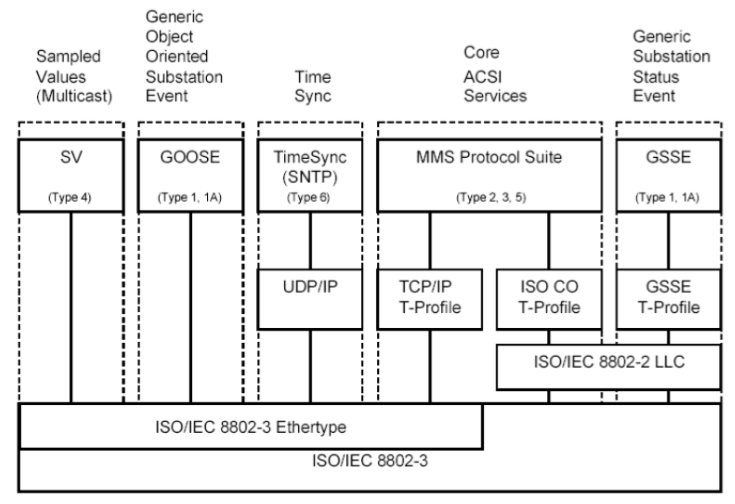
\includegraphics[scale=0.350]{imgs/tools_iec61850.png}
	\caption{Tools di IEC 618504} \label{fig:tools_iec61850}
\end{figure}
\textbf{GSE} è un protocollo che fornisce uno strumento veloce ed affidabile per la segnalazione di \emph{eventi} all'interno della sottostazione. Le caratteristiche principali sono il servizio multicast/broadcast con modello di comunicazione publish/subscribe. I messaggi sono trasmessi in formato binario. GSE prevede due modelli di servizio che prendono il nome di GOOSE e GSSE.\newline\newline
\textbf{GOOSE} è stato progettato per essere \emph{brand indipendent}. Utilizza Virtual LAN, stabilendo più network virtuali sulla stessa rete fisica e determinando livelli di priorità per i messaggi, consentendone anche la ritrasmissione (un identificativo indica se il messaggio è nuovo o ritrasmesso).\newpage
\textbf{GSSE} è utilizzato per lo scambio di informazioni sui soli cambiamenti di stato. In questo caso i messaggi sono costituiti da una serie di bit che rappresentano liste di stati. GSSE necessita un tempo di trasmissione maggiore se confrontato con GOOSE.
\newline\newline
\textbf{SMV} è un protocollo per lo scambio di dati e la trasmissione di misure prodotte dai trasduttori delle sottostazioni: permette lo scambio di segnali tra gli IED. Prevede due metodi di comunicazione:
\begin{itemize}
	\item\emph{SV over Serial Unidirectional Multidrop Point-to-Point fixed link}: Sistema di comunicazione unidirezionale che specifica una serie di dataset (tensioni trifase, correnti trifase, etc). I valori analogici vengono codificati a 16 bit;
	\item\emph{SV over Ethernet}: Versione più generica e flessibile di SV che fornisce la possibilità di definire dataset con valori di diversa dimensione e tipo, configurabili dall'utente grazie all'utilizzo di SCL. Utilizza un modello di comunicazione publish/subscribe con possibilità di multi-casting.
\end{itemize}
\textbf{Time Synchronization} è un servizio di sincronizzazione dei clock fondamentale per applicazioni real-time. Utilizza un subset di Network Time Protocol (NTP) con riferimento allo Universal Coordinated Time (UTC). NTP è il protocollo tipicamente utilizzato per sincronizzare i clock di computer collegati ad Internet e in LAN.\newline\newline
\textbf{Report} è lo strumento che permette di memorizzare i cambiamenti dei dati e degli attributi relativi ai nodi logici. Genera dataset contenenti attributi di interesse e richiede ai nodi logici l'invio delle informazioni riguardanti le variazioni nel sistema.\newline\newline
\textbf{Log} è la registrazione degli eventi relativi ad un dispositivo. I log sono registrati in un server e, a differenza dei Report, i dispositivi logici creano al loro interno un database di eventi senza inviarne notifica.\newline\newline
Tra i limiti di IEC 61850 si evidenziano i costi elevati per l'installazione dei server e dei dispositivi atti alla gestione dei dati ma anche  complessità dal punto di vista dell'architettura. IEC 61850 è affiancato da IEC 62351 che garantisce la sicurezza e specifica i requisiti tecnici che devono essere rispettati dai fornitori.
\newpage
\section{Standard per la sicurezza}
Gli standard per la sicurezza informatica sono di recente invenzione e fondamentali data la grande mole di informazioni sensibili memorizzate sui computer che sono collegati ad Internet. Inoltre, molte attività che prima erano condotte manualmente, oggi sono svolte dalle macchine in maniera automatica introducendo quindi un maggiore bisogno di affidabilità e di sicurezza in tali sistemi informatici. La sicurezza è un fattore importante per per gli individui che devono proteggersi dal cosiddetto furto di identità ma anche per le aziende perché devono proteggere i loro segreti industriali e le informazioni sui dati personali dei clienti.\newline\newline
I problemi relativi alla sicurezza vanno dagli accessi non autorizzati a informazioni recuperate dagli smart meter, lo spegnimento dei dispositivi da parte di un attaccante così come un attacco alla Smart Grid per causare un'interruzione al passaggio di corrente. I problemi relativi alla privacy riguardano invece l’alta frequenza con cui vengono effettuate le letture per misurare il consumo energetico in quanto esse mostrano totalmente il comportamento dell’utente. In generale si cerca di aggregare le informazioni dei meter per rilevare sia frode che perdite (per esempio nel caso del gas, dove un'eventuale perdita pone un problema di sicurezza) utilizzando schemi di aggregazione \emph{privacy-friendly} in modo da mascherare i singoli consumi dei meter.
\newline\newline
Nell'ambito dei power system, esistono diversi standard che si applicano alla sicurezza delle apparecchiature all'interno delle sottostazioni e molti sono in fase di sviluppo. Per la valutazione complessiva della sicurezza, è ampiamente utilizzata la norma ISO 27001 e specifica la valutazione dei rischi e la strategia da utilizzare per lo sviluppo di un sistema di sicurezza in modo da limitarli.
\subsection{IEC 62351}
IEC 62351 è uno standard sviluppato dal WG15 facente parte della TC57 dell'organo internazionale IEC. Questo standard è stato sviluppato per gestire la sicurezza nella serie di protocolli della commissione tecnica 57, tra i quali le serie IEC 60870-5, IEC 60870-6 series, IEC 61850, IEC 61970 e IEC 61968.\newpage
Tra i diversi obiettivi di sicurezza che lo standard persegue ci sono:
\begin{itemize}
	\item Autenticazione nel processo di trasferimento di dati tramite firma digitale;
	\item Garanzia di accessi esclusivamente dopo autenticazione;
	\item Prevenzione dell'eavesdropping (ossia intercettazioni della comunicazione non autorizzate);
	\item Prevenzione da attacchi di playback e attacchi di spoofing (ovvero sostituirsi ad una controparte della comunicazione);
	\item Rilevamento delle intrusioni.
\end{itemize}
Le prime due parti di IEC 62351 comprendono la spiegazione di differenti scenari e la definizione di alcuni termini. IEC 62351 utilizza i protocolli di sicurezza esistenti, come il Transport Layer Security (TLS, \cite{tls}), utilizzato con successo in altre aree tecniche e in diverse parti dello standard. TLS prevede servizi di sicurezza come la mutua autenticazione dei peer in una comunicazione (utile per contrastare attacchi man-in-the-middle) ma si occupa anche dell'integrità e della riservatezza dei dati comunicati. La terza parte di IEC 62351 definisce come possono essere forniti servizi di sicurezza in una  comunicazione TCP/IP based e specifica suite di cifratura. La quarta parte specifica le procedure, i miglioramenti del protocollo, e gli algoritmi atti a promuovere l'aumento dei messaggi di sicurezza trasmessi su MMS. Questa parte definisce alcune procedure relative a Transport e Application Layer, basate su TLS, in modo da proteggere le informazioni trasmesse. La quinta parte riguarda invece la comunicazione seriale in cui si vanno a definire ulteriori misure di sicurezza per proteggere l'integrità delle connessioni seriali applicando chiavi hash. Questa parte specifica quindi anche una separata gestione delle chiavi. La sesta parte di IEC 62351 si occupa dei profili di IEC 61850 per la comunicazione, non basati su TCP/IP. La settima parte è utile poichè implementa e/o estende sistemi di intrusion detection e l'ottava e ultima parte si occupa di role-based access control.
%La Figura \ref{fig:62351} mostra un overview sulle differenti parti che compongono lo standard.
%\begin{figure}[h]
%	\centering
%	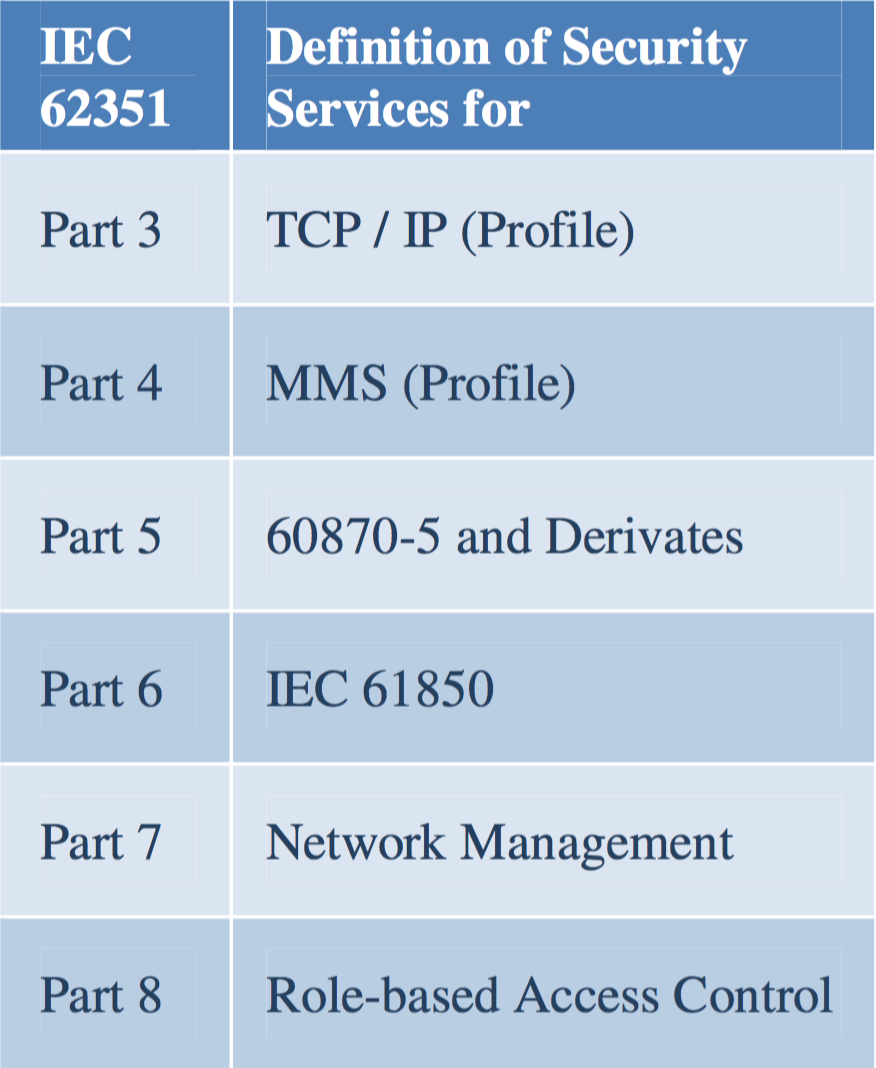
\includegraphics[scale=0.350]{imgs/62351.png}
%	\caption{Overview IEC 62351} \label{fig:62351}
%\end{figure}

\begin{thebibliography}{99}
\bibitem{802.3} \url{http://www.ieee802.org/minutes/2011-March/802\%20workshop/index.shtml}.
\bibitem{zb} ZigBee Specification, ZigBee Alliance, ZigBee Document 053474r17, January 2008.
\bibitem{wimax} Cudak, M. (ed.) (2010) IEEE 802.16m System Requirements, IEEE 802.16 Task Group M, January 2010, \url{http://ieee802.org/16/tgm/docs/80216m-07_002r10.pdf}.
\bibitem{dnp} IEEE Power \& Energy Society (2010) IEEE Std 1815TM-2010: IEEE Standard for Electric Power Systems Communications-Distributed Network Protocol (DNP3), June.
\bibitem{iec61850} IEC 61850 - communication networks and systems in substation: an overview of computer science.
University of Illinois at Urbana Champaign, jan. 2010. %presentation
\bibitem{tls} RFC 5246: The Transport Layer Security (TLS) Protocol, Version 1.2, T. Dierks, E Rescorla, August 2008
\end{thebibliography}
\chapter{Principali vulnerabilità delle Smart Grid: attacchi e contromisure}
% !TeX spellcheck = it_IT
Negli ultimi anni, un numero sempre crescente di infrastrutture critiche è stato digitalizzato, aggiungendo capacità di comunicazione e di computazione a numerosi dispositivi nelle reti di distribuzione dell'energia e dell'acqua, sistemi di trasporto, e manifatturieri. Ciò avviene in parte con lo scopo di aumentare l'efficienza, ma spesso è anche un requisito necessario a gestire l'ambiente che muta, come ad esempio la generazione locale dell'energia o il passaggio ai veicoli elettrici nel caso della distribuzione energetica.\\
Un progetto di digitalizzazione molto visibile è il passaggio dai \emph{meter} analogici ai digitali (\emph{smart}), che è attualmente in corso in vari paesi del mondo. Oltre ad una fatturazione complessivamente più precisa, uno smart meter può anche dare input agli algoritmi di controllo della grid, essere usato nei mercati energetici, comunicare con la \emph{smart home} (ad esempio, per regolare l'aria condizionata ed i sistemi di riscaldamento quando la richiesta energetica è alta), oppure per disconnettere da remoto un consumatore. In questo modo, un dispositivo precedentemente disconnesso e non critico si trasforma in un dispositivo connesso che può generare dati \emph{process-critical}.\\
La robustezza dei dati e dei comandi di switch è vitale - se una grande quantità di famiglie viene disconnessa simultaneamente, l'energia in eccesso non ha dove andare, potrebbe danneggiare la grid. In maniera simile, se gli algoritmi di manutenzione si basano su dati provenienti da misure effettuate dagli smart meter, input errati possono produrre effetti di gran lunga peggiori delle frodi di fatturazione. Ciò pone una nuova sfida per i produttori di meter: progettare dispositivi economici, largamente distribuiti e che lavorino su canali con banda molto ristretta.
\section{Open Smart Grid Protocol \label{sez:OSGP}}
L'Open Smart Grid Protocol (OSGP) \cite{osgp} è un protocollo di comunicazione per smart grid costruito sullo stack protocollare ISO/IEC 14908-1 \cite{standard14908}, sviluppato dalla Energy Service Network Association (ESNA), ed è uno standard dell'European Telecommunications Stardards Institute (ETSI) fin dal 2012. È stato uno dei primi protocolli di comunicazione su powerline per smart meters disponibile sul mercato, ed è largamente utilizzato per comunicare tra smart meter e l'aggregatore di dati, il quale è un dispositivo che colleziona dati provenienti da diverse centinaia di meter in un segmento di PLC (Power Line Communication) e li inoltra ad un controllore centralizzato.\\
Nonostante l'OSGP sia principalmente utilizzato per applicazioni di smart-metering, esso è stato progettato per un utilizzo più ampio all'interno di dispositivi della Smart Grid. Lo stack protocollare è molto leggero. Tale leggerezza è ottenuta pagando in sicurezza, infatti le primitive crittografiche consigliate dal NIST  (ad esempio: Advanced Encryption Standard - AES, in \emph{authenticated mode}) sono evitate, optando per altre meno intense computazionalmente: lo stream cipher RC4 per la cifratura ed una funzione digest non standard per l'autenticazione dei messaggi.\\
%\emph{authenticated encryption} (AE) è la tecnologia standard per proteggere dati che devono essere inviati su canali di comunicazione non sicuri, ed è utilizzata in un gran numero di applicazioni, come ad esempio TLS, SSH ed IPSec. In confronto ai regolari schemi di cifratura simmetrica, AE non solo assicura la \emph{privacy} del dato ma inoltre garantisce l'integrità e l'autenticità. Sfortunatamente, errori di progettazione ed implementazione degli schemi di AE sono noti e ne esistono numerosi esempi. Per nominarne solo alcuni:
%\begin{itemize}
%	\item Vaudenay 2002. Attacco CBC padding oracle al MAC-then-encrypt AE mode, consente ad un avversario di decifrare i messaggi senza accedere alla chiave segreta \cite{cbcpadding}. Questo attacco è derivato dalla mancanza di verifica di autenticità nel caso in cui il messaggio avesse il padding adeguato. Negli anni, tale strategia è stata utilizzata con successo contro TLS.
%	\item Nel 2007, un attacco \cite{wep2} al Wired Equivalent Privacy (WEP) standard, utilizzato nella maggior parte delle reti Wi-Fi 802.11, consentiva di recuperare la chiave segreta in pochi minuti a partire da poche migliaia di messaggi intercettati. L'attacco sfruttava delle debolezze in RC4.
%\end{itemize}
In OSGP si introducono misure per proteggere la \textit{privacy} dei clienti, restringendo l'accesso ai dati e cifrando questi ultimi per evitare che persone non autorizzate possano modificarli. Si introducono, inoltre, misure per rintracciare potenziali tentativi di eludere le funzioni di metering, che potrebbero risultare in accessi non registrati ai servizi. \newline Come detto in precedenza, OSGP è costruito sullo stack protocollare ISO/IEC 14908-1, che fornisce servizi di autenticazione, ma non include meccanismi per garantire la confidenzialità dei dati. Per questo motivo, OSGP completa la sicurezza di questo standard, aggiungendo un proprio \textit{security layer} che fornisce autenticazione e confidenzialità \cite{osgpsec}.\\
Il protocollo OSGP si suddivide in:
\begin{itemize}
\item \textit{Setup}, in cui si effettua la configurazione iniziale degli smart meter e del data concentrator;
\item \textit{Communication with authenticated encryption}, in cui gli smart meter comunicano con i data concentrator utilizzando meccanismi di autenticazione e di cifratura dei dati.
\end{itemize}

\subsection{Setup}
Durante il processo di produzione industriale, i dispositivi OSGP vengono configurati con una \textit{Open Media Access Key} (OMAK) univoca a 96 bit. Tali chiavi sono poi consegnate in maniera sicura alle società di servizi, che provvedono poi a dotare il proprio data concentrator della chiave OMAK del dispositivo afferente alla zona di competenza. \newline Il data concentrator è in grado di rilevare ogni dispositivo a lui afferente grazie ad un processo di discovery; successivamente, genera ed invia la Shared Key relativa alla sua zona di competenza ad ogni nuovo dispositivo scoperto. Tale comunicazione avviene in maniera cifrata, utilizzando come chiave di cifratura la OMAK del dispositivo. Ogni dispositivo, poi, rimpiazza la sua OMAK originaria con la Shared Key ricevuta. \newline La Shared Key è utilizzata per i seguenti scopi:
\begin{itemize}
\item Per l'autenticazione di messaggi;
\item Come chiave in input per l'OSGP OMA Digest Algorithm;
\item Per la cifratura: dall'OMAK, si deriva inizialmente una Base Encryption Key (BEK) a 128 bit che, successivamente, si combina in XOR con un OSGP digest, per produrre la chiave di cifratura di RC4.
\end{itemize}

\subsection{Communication with authenticated encryption \label{subsec:OSGPauth}}
OSGP è un protocollo master - slave, in cui il master è rappresentato dal data concentrator e lo slave dallo smart meter, che si basa sulla Shared Key per cifrare i messaggi scambiati durante la comunicazione. In particolare, la comunicazione è iniziata dal data concentrator il quale invia un messaggio di richiesta cifrato allo smart meter; successivamente, lo smart meter decifra il messaggio, ne verifica l'autenticità (vedi paragrafo Authentication) e invia la risposta, anch'essa opportunamente cifrata. Smart meter e data concentrator sono identificati dai campi Subnet e Node ID del pacchetto di richiesta/risposta.
\subsubsection{6.1.2.1 Authentication}
Il data concentrator OSGP utilizza autenticazione basata su digest a livello applicativo per autenticare messaggi del livello applicazione tra i dispositivi. Questa forma di autenticazione richiede la metà dei pacchetti richiesti dall'autenticazione EN 14908. Per evitare replay attack, viene effettuato l'\emph{append} di un sequence number al \emph{payload} e successivamente se ne effettua il digest complessivo.\\
Quando il device è in fase di inizializzazione sceglie un proprio sequence number iniziale casuale. Assumendo che il dispositivo si aspetti un sequence number $N$, esso rifiuta qualsiasi messaggio che non abbia sequence number compreso tra $N-1$ ed $N+M$, dove $M$ è pari ad 8. Quando è ricevuta una richiesta con sequence number $N-1$, la response per tale richiesta inviata originariamente, se presente, viene nuovamente inviata. Se il sequence number ricevuto in una richiesta è fuori dal range specificato ($[N-1, N+M]$), il dispositivo risponderà a tale richiesta con una NACK response contenente il messaggio di ``\emph{invalid sequence number}'', seguita dal sequence number desiderato. A quel punto sta al data concentrator iniziare ad usare il nuovo sequence number.\\
Le richieste rispettano il seguente formato:
\begin{table}[!h]
	\centering
%	\caption{My caption}
%	\label{my-label}
	\begin{tabular}{|l|l|l|}
		\hline
		Request & Sequence (4 byte) & Digest (8 byte) \\ \hline
	\end{tabular}
\end{table}
\newline
Il digest nella fase di request è computato sui dati seguenti, utilizzando l'Algoritmo \ref{oma_algo1} che fa uso della OMA key a 96 bit.\\
\begin{table}[!h]
	\centering
	%	\caption{My caption}
	%	\label{my-label}
	\begin{tabular}{|l|l|l|l|}
		\hline
		Subnet (1 byte) & Node (1 byte) & Request & Sequence\\ \hline
	\end{tabular}
\end{table}
\newline
Le response seguono il seguente formato:
\begin{table}[!h]
	\centering
	%	\caption{My caption}
	%	\label{my-label}
	\begin{tabular}{|l|l|l|}
		\hline
		Response & Digest (8 byte)\\ \hline
	\end{tabular}
\end{table}
\newline
\newline
Il digest nella fase di response è computato sui seguenti dati, utilizzando come prima l'Algoritmo \ref{oma_algo1}:
\begin{table}[!h]
	\centering
	%	\caption{My caption}
	%	\label{my-label}
	\begin{tabular}{|l|l|l|l|l|l|}
		\hline
		Subnet (1 byte) & Node (1 byte) & Request & Sequence & Response & Response Length (1 byte)\\ \hline
	\end{tabular}
\end{table}
\newline
Da notare che anche le response NACK sono rese sicure nel modo che abbiamo appena visto.\\
I dispositivi OSGP possono inviare i seguenti tipi di NACK:\\
``Subnet'' e ``Node'' nei diagrammi visti sopra si riferiscono sempre a subnet/node del target della richiesta. Ovvero, è lo stesso indirizzo in entrambe le direzioni. ``Request'' e ``Sequence'' fanno riferimento sempre ai valori nel messaggio di richiesta originale.\\
Si assume che il dispositivo possa mantenere il suo sequence number per più riavii (\emph{power cycle}). Quindi, il primo messaggio autenticato in seguito all'accensione richiederà uno scambio extra.\\
Tutti i dati dei device critici sono protetti dall'autenticazione basata su digest al livello applicativo sia per operazioni di lettura che di scrittura. Questo include:\\
\begin{itemize}
	\item Configurazione di un dispositivo OSGP
	\item Fatturazioni e profili di carico OSGP
	\item Richieste di cancellazione del carico
	\item Time setting
\end{itemize}
Le seguenti operazioni sono protette attraverso la \textit{challenge authentication} di EN 14908. Questa verifica dell'autenticazione è responsabilità dell'interfaccia EN 14908, e non del dispositivo OSGP:
\begin{itemize}
	\item Indirizzamento logico di EN 14908
	\item Modifica della authentication key
	\item Misura di fase
	\item Impostazioni di compatibilità
	\item Cambio della modalità del nodo
	\item Letture/Scritture in memoria
\end{itemize}
Le seguenti operazioni non sono protette da autenticazione:
\begin{itemize}
	\item Query di stato EN 14908
	\item Misure della potenza del segnale
\end{itemize}
\subsubsection{6.1.2.2 Encryption}
Si analizza quindi lo schema di \emph{authenticated encryption} utilizzato nell'Open Smart Grid Protocol.\\
Tale schema si suddivide in una parte di autenticazione ed una di cifratura e si basa su tre algoritmi: l'algoritmo EN 14908 \cite{standard14908}, lo stream cipher RC4 ed il digest OMA, quest'ultimo è un \emph{message authentication code} (MAC). Questi tre algoritmi sono combinati secondo gli approcci \textit{MAC-and-encrypt} e \textit{MAC-then-encrypt}, a formare uno schema di cifratura autenticata. Da notare che, mentre il digest OMA è descritto nella specifica OSGP \cite{osgp}, informazioni pubbliche riguardo l'algoritmo EN 14908, specificato in ISO-IEC 14908-1 \cite{standard14908}, sono difficili da recuperare. Tutte le informazioni su quest'ultimo sono state ottenute dalla specifica OSGP.\\
%Il problema più grande è la combinazione di uno stream cipher con una funzione di digest lineare, che apre le possibilità per attacchi alle chiavi crittografiche ed ai messaggi. Ad esempio, si potrebbe sfruttare tale vulnerabilità utilizzando il ricevente di un messaggio come un ``oracolo". Dato un messaggio propriamente cifrato ed autenticato, un attaccante ipotizza una combinazione di un bit del messaggio ed un bit della chiave, invia un messaggio, appositamente confezionato, al ricevente ed utilizza la risposta del  dispositivo che rifiuti o confermi l'ipotesi. Siccome questo può essere effettuato per singoli bit, un attaccante può ricostruire la chiave principale del dispositivo (OMA key) con al più $96 \times 3$ risposte.
\paragraph{6.1.2.2.1 Notazione}\mbox{}\\
Una stringa $x$ di $n$ bit è un elemento di $\{0,1\}^n$. La taglia di $x$ in bit è denotata da $|x|$. La concatenazione di stringhe di bit è identificata da $||$. Dato un vettore di stringhe di bit $(x_0, \ldots, x_{n-1})$, si denota con $x_{i,j}$ il $j$-esimo bit della $i$-esima stringa dove $0 \leq i \leq n-1$. Quando si le stringhe di bit sono interpretate come interi si utilizza il formato little-endian denotato in esadecimale.\\
Una stringa di bit composta da $n$ zero è denotata da $0^n$.\\
Una rotazione ciclica di una stringa di bit $x$ di $m$ bit verso sinistra e destra sono denotate con $x \lll m$ ed $x \ggg m$, rispettivamente. La differenza di due stringhe di bit $x$ ed $x^\prime$ rispetto allo XOR è denotata da $\Delta x$, mentre la differenza rispetto all'addizione modulo $2^n$ è denotata da $\delta^{\boxminus}x$.
\paragraph{6.1.2.2.2 Infrastruttura Crittografica di OSGP}\mbox{}\\
La struttura ad alto livello dello schema di cifratura autenticata (AE) di OSGP è mostrata in Figura \ref{osgp_img}.
\begin{figure}[hbtp]
	\centering
	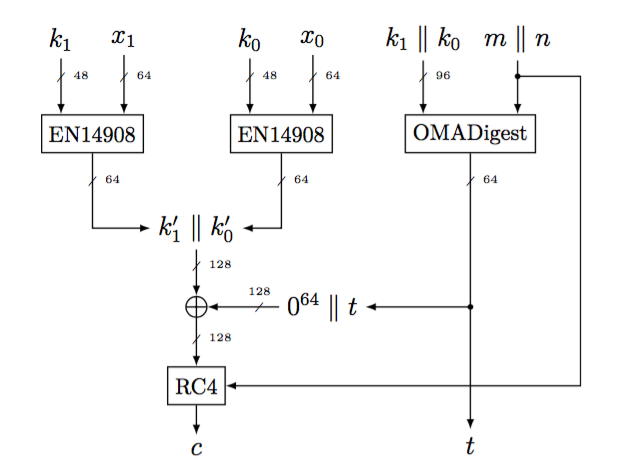
\includegraphics[scale=.5]{imgs/attack/osgp.png}
	\caption{Lo schema AE di OSGP. Notazione: $x_0 = \{${\tt 81, 3F, 52, 9A, 7B, E3, 89, BA}$\},$ $x_1 = \{${\tt 72, B0, 91, 8D, 44, 05, AA, 57}$\},$ $k = k_1 \| k_0$ : Open Media Access Key (OMAK), $m$: messaggio, $n$: numero di sequenza, $t$: tag di autenticazione, $k^\prime = k^{\prime}_{1} \| k^{\prime}_{0}$: Base Encryption Key (BEK), $c$: ciphertext.}
	\label{osgp_img}
\end{figure}
La sicurezza dello schema AE di OSGP dipende dalla \textit{Open Media Access Key} (OMAK) a 96 bit $k = k_1 \| k_0$, da cui deriva tutto ciò legato alla chiave. La OMAK è solitamente univoca per ogni device ma non \textit{hardcoded} e può essere cambiata.\\
Dalla OMAK derivano due cose: inizialmente, è computata una \emph{Base Encryption Key} (BEK) $k^\prime =  k^{\prime}_{1} \| k^{\prime}_{0}$, che è una chiave a 128 bit che compone la base della chiave di cifratura di RC4. La BEK è costruita (la specifica OSGP non è chiara su come la BEK sia rilevata, la descrizione presentata è basata sulle investigazioni svolte in \cite{dumbcrypto}. L'osservazione chiave qui è che la BEK è derivata dall'OMAK. Non è importante il modo, ed è solamente descritto per completezza) utilizzando l'algoritmo EN 14908, che sembra essere la base dell'OMA digest ma usa chiavi più piccole a 48 bit e processa i byte dei messaggi in ordine inverso. L'algoritmo EN 14908 è applicato ad ognuna delle metà $k_0$ e $k_1$ dell'OMAK e delle due costanti $x_0 = ${\tt \{ 81, 3F, 52, 9A, 7B, E3, 89, BA \}}, ed $x_1 = $ {\tt \{ 72, B0, 91, 8D, 44, 05, AA, 57 \}}. I due risultati a 64 bit sono concatenati per formare $k^{\prime}$, come mostrato in Figura \ref{osgp_img}. La BEK dipende solo dall'OMAK ed è quindi fissata fin quando $k$ resta invariato.\\
In secondo luogo, un tag di autenticazione $t$ è prodotto utilizzando il digest OMA sul messaggio $m$ concatenato ad una \emph{sequence number} $n$ e la OMAK $k$. Si denoti con $l$ la taglia di $m\|n$ in byte. Il digest OMA inizia con gli 8 byte $a = (a_0, \ldots, a_7)$ del suo stato interno impostati a 0. Per prima cosa, $m\|n$ è \emph{zero-padded} ad un multiplo di 144 byte, cioé\\
\indent $m^\prime = m \| n \| 0^{-l\, mod\, 144}$.\\
Il primo, e potrebbe anche ultimo, blocco da 144 byte del messaggio è denotato da $m^\prime = m^\prime_0 \| \cdots \| m^\prime_{143}$. Lo stato interno è continuamente aggiornato utilizzando una funzione nonlineare $f_{b,c}$ dove $b = k_{i\, mod\, 12, 7-j}$ è un bit chiave e $c = j$ è la posizione corrente nello stato. La sua specifica è riportata di seguito:\\
\indent   $f_{b,c}(x,y,z)=
\begin{cases}
	y + z + (\neg(x + c)) \lll 1\quad if\quad b=1\\
	y + z - (\neg(x + c)) \ggg 1\quad altrimenti.
\end{cases}$\\
Per aggiornare l'elemento di stato $a_j$, la funzione $f$ prende, per $0 \leq i \leq 17$ e $7 \geq j \geq 0$, due elementi di stato adiacenti $a_j$ ed $a_{j+1\, mod\, 8}$ ed un byte del messaggio $m^\prime_{8i+7-j}$ in input, ad esempio, $a_j = f_{k_{i\,mod\,12,7-j},j}$, ed in funzione del valore del bit chiave $k_{i\,mod\,12,7-j}$ uno dei due rami mostrati sopra viene valutato. Il prossimo blocco da 144 byte del messaggio è processato in maniera simile, con lo stato interno proveniente dal blocco precedente. Lo pseudocodice del digest OMA è mostrato nell'Algoritmo \ref{oma_algo1} ed una visualizzazione del ciclo più interno, dove i byte del messaggio sono processati, è mostrata in Figura \ref{inneroma_img}.
\begin{figure}[hbtp]
	\centering
	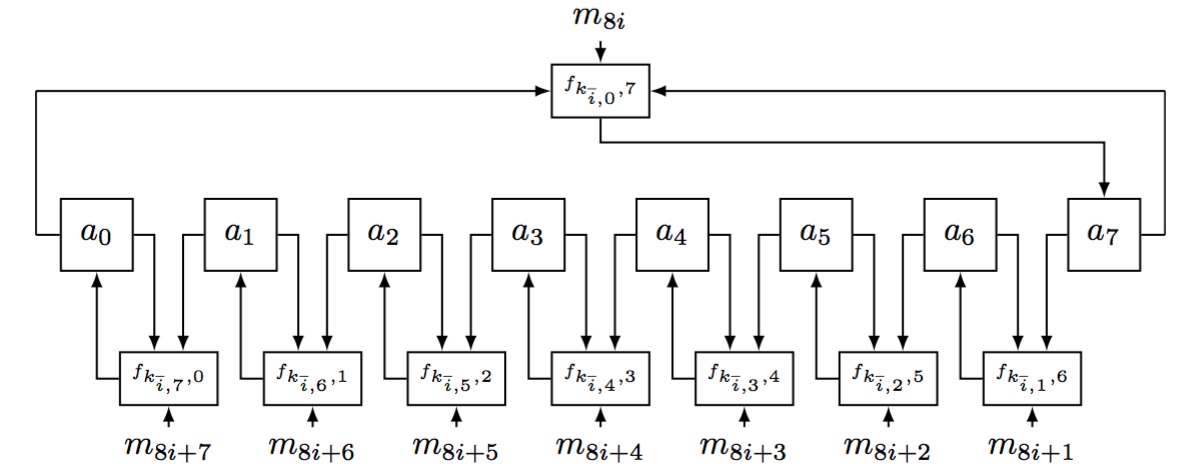
\includegraphics[scale=.3]{imgs/attack/oma_innerloop.png}
	\caption{Processing dei dati (da destra verso sinistra) nel digest OMA, con $\bar i = i\,mod\,12$.}
	\label{inneroma_img}
\end{figure}
Dopo la generazione del tag $t$, ne viene effettuato lo XOR con la metà bassa della BEK $k^\prime$ che poi produce la chiave di cifratura di RC4 a 128 bit $k^{\prime} = k^\prime_1 \| (k^\prime_0 \oplus t)$, come mostrato in Figura \ref{osgp_img}.
\begin{algorithm}[H]
\Fn{{\tt OMADigest} ($m,\,k$)}{
	$a \gets (0,0,0,0,0,0,0,0)$\\
	$m \gets m\,\|\,0^{-|m|\,mod\,144}$\\
	\ForEach{144-byte block b of m}{
		\For{$i \gets 0$ \KwTo 17}{
			\For{$j \gets 7$ \KwTo 0}{
				\eIf{$k_{i\,mod\,12,7-j} = 1$}
				{$a_j \gets a_{(j+1)\,mod\,8}+b_{8i+(7-j)}+(\neg(a_j+j)) \lll 1$}
				{$a_j \gets a_{(j+1)\,mod\,8}+b_{8i+(7-j)}-(\neg(a_j+j)) \ggg 1$}
				}
			}
		}
	\Return{a}
	}
\caption{Il digest OMA di OSGP. $a$ 8 byte (output tag della funzione), $a_j$ e $j$ ognuno da 8 bit, $\neg(a_j+j)$ negazione bit a bit della rappresentazione binaria della somma dei due interi da 8 bit.}
\label{oma_algo1}
\end{algorithm}\mbox{}\\
Questa scelta è intesa per fornire ad RC4 materiale chiave in continuo cambiamento, così producendo un \textit{keystream} nuovo ad ogni messaggio, per cui, in accordo alla specifica OSGP, il numero di sequenza $n$, concatenato ad $m$, è continuamente incrementato.\\
I sequence number sono condivisi tra mittente e destinatario in OSGP. Il destinatario di un messaggio verifica che il corretto sequence number sia stato concatenato a quest'ultimo. I messaggi con sequence number nel range $\{n, \ldots, n+8\}$ sono accettati come richieste valide. Se un messaggio con sequence number $n-1$ è ricevuto, il destinatario non esegue la richiesta, ma reinvia la risposta della richiesta (eseguita precedentemente) numero $n-1$. I numeri di sequenza fuori di tale range fanno scattare un errore ed i dispositivi OSGP rispondono con un codice di fallimento ed il corretto sequence number.\\
Dopo che la fase di setup è terminata, $k^{\prime\prime}$ è utilizzato per cifrare $m\|n$ tramite RC4 per ottenere il ciphertext $c$. Infine, $c\|t$ è trasmesso. La taglia massima consentita dei messaggi $m\|n$ processati in OSGP è di 114 byte.
\newpage
\subsection{Analisi}
OSGP utilizza RC4 per la cifratura. RC4 è soggetto ad attacchi di \textit{statistical key recovery} e \textit{plaintext key recovery}, ed è dimostrato come tali siano fattibili \cite{rc4tls}, \cite{weakrc4}, \cite{rc4rand}, \cite{rc4statistical}. Comunque, in questa analisi non ci si concentra su RC4, ma sul digest OMA (vedi Algoritmo \ref{oma_algo1}). L'algoritmo del digest OMA presenta più falle. Per iniziare, utilizza un semplice padding a zero byte, che risulta in messaggi con un qualsiasi numero di zeri finali che condividono lo stesso tag. Inoltre, data una tupla $(a, m, k)$ dove $a$ è lo stato del digest OMA o il tag di autenticazione, $m$ un messaggio e $k$ la OMAK, la funzione non impedisce agli attaccanti di ottenere il messaggio originale (si veda l'Algoritmo \ref{oma_algo2}) il che è una proprietà molto comoda per loro. Allo stesso modo, è anche possibile prendere uno stato interno arbitrario e continuare a processarlo come per riprendere un messaggio di cui si è fatto un digest parziale. Ciò è mostrato nell'Algoritmo \ref{oma_algo3}.
\begin{algorithm}[!h]
	\Fn{{\tt OMABackward} ($a,m,k,n$)}{
		\tcc{Assumes $|m|\leq144$}
		$m \gets m\,\|\,0^{-|m|\,mod\,144}$\\
		\For{$l \gets 0$ \KwTo $n-1$}{
			$i,j \gets \lfloor l/8\rfloor,\,l\,mod\,8$\\
			\eIf{$k_{(17-i)\,mod\,12,7-j} = 1$}
				{$x \gets (a_j - a_{(j+1)\,mod\,8}-m_{143-8i-j}) \ggg 1$}
				{$x \gets (a_{(j+1)\,mod\,8}+m_{143-8i-j}-a_j) \lll 1$}
			$a_j \gets \neg x - j$
		}
		\Return{a}
	}
	\caption{Il ``backward'' digest OMA di OSGP, ripristina lo stato interno di $n$ byte dei messaggi.}
	\label{oma_algo2}
\end{algorithm}
\newpage
\begin{algorithm}[!h]
	\Fn{{\tt OMAForward} ($a,m,k,n$)}{
		\tcc{Essentially Algorithm \ref{oma_algo1}, but start at byte $m_n$ with a known state $a$, and assume $|m| \leq 144$.}
		$m \gets m\,\|\,0^{-|m|\,mod\,144}$\\
		\For{$l\gets n$ \KwTo 143}{
			$i,j \gets \lfloor l/8\rfloor,\,7-l\,mod\,8$\\
			\eIf{$k_{i\,mod\,12,7-j} = 1$}
				{$a_j \gets a_{(j+1)\,mod\,8}+m_{8i+7-j}+(\neg(a_j+j)) \lll 1$}
				{$a_j \gets a_{(j+1)\,mod\,8}+m_{8i+7-j}-(\neg(a_j+j)) \ggg 1$}
		}
		\Return{a}
	}
	\caption{Il ``forward'' digest OMA di OSGP, inizia con uno stato iniziale noto e processa byte di messaggi a partire dalla posizione $n$.}
	\label{oma_algo3}
\end{algorithm} 
Di seguito è riportato un attacco mirato a recuperare la OMAK, mediante cifratura di un testo in chiaro scelto dall'attaccante.
\subsubsection{Chosen-Plaintext Key Recovery Attack}
Sia $a=\left(a_0,\ldots,a_7\right)$ lo stato interno a 8 byte del digest OMA. L'attacco discusso in seguito, utilizza messaggi scelti a 144 byte della forma $m=m_0 \|\cdots \|m_{143}$ e sfrutta le debolezze differenziali nel digest OMA.
\newline \newline
\textbf{Bitwise Key Recovery}.
Tale attacco recupera l'intera chiave un bit alla volta, attraverso la crittoanalisi differenziale. Nello specifico, sfrutta lo XOR-\textit{differential}$\left(\Delta_{m_i}, \Delta_{a_j}\right) =\,$\texttt{(80,80)}, in cui $\Delta_{m_i}$ e $\Delta_{a_j}$ sono, rispettivamente, le differenze in input e output per j = 7-i mod 8. La differenza in output è ottenuta subito dopo il \textit{processing} del byte $m_i$ del messaggio (vedi Algoritmo \ref{oma_algo1}), e può essere scritto come
\begin{equation*}
\begin{split}
&f_{k,j}\left(a_j, a_{j+1 \, mod \, 8}, m_i \oplus \texttt{80} \right) \\
=\,&a_{j+1\,mod\,8} + \left( m_i \oplus \texttt{80} \right) \, \pm \, \left(\texttt{FF} \oplus (a_j+j) \lll r \right) \\
=\,&\left(a_{j+1\,mod\,8} + m_i \pm ( \texttt{FF} \oplus (a_j+j) \lll r)\right)\oplus \texttt{80} \\
=\,&f_{k,j}\left(a_j, a_{j+1 \, mod \, 8}, m_i\right) \oplus \texttt{80}
\end{split}
\end{equation*}
in cui la rotazione ciclica $r\,\in \, \{1,7\}$ e l'operazione $\pm$, dipendono dal valore del bit chiave $k \, \in \, \{0,1\}$. Questo XOR-\textit{differential} ha probabilità 1, in accordo a proprietà differenziali ben note dell'addizione modulo $2^n$ \cite{diff}, e si propaga nettamente attraverso lo stato \textit{a} per le successive 8 iterazioni, restituendo come risultato la seguente differenza
\begin{equation*}
\Delta_a \, = \, (\texttt{80},\texttt{80},\texttt{80},\texttt{80},\texttt{80},\texttt{80},\texttt{80},\texttt{80}).
\end{equation*}
L'iterazione successiva dell'algoritmo rivela un bit chiave della OMAK. Linearizzando attraverso lo XOR la funzione \textit{f} di aggiornamento dello stato, la nuova differenza in output $\Delta_{a'_j}$ è della forma
\begin{equation*}
\begin{split}
\Delta_{a'_j} \, = \, & ((a_{j+1 \, mod \, 8} \oplus \texttt{80}) \oplus m_i \oplus (\texttt{FF} \oplus ((a_j \oplus \texttt{80}) \oplus j) \lll r)) \, \oplus \\
&(a_{j+1 \, mod \, 8} \oplus m_i \oplus (\texttt{FF} \oplus (a_j \oplus j) \lll r))
\end{split}
\end{equation*}
dove $r\,\in \, \{1,7\}$. Di conseguenza, si ha che $\Delta_{a'_j}\,=\,\texttt{81}$ se il bit 7-i mod 8 di $k_{\lfloor i/8 \rfloor \, mod \, 12}$ è pari a 1, e $\Delta_{a'_j}\,=\,\texttt{C0}$, se lo stesso bit chiave è 0. Sebbene l'addizione e lo XOR tra interi si comportino diversamente rispetto alla propagazione delle differenze XOR, il bit meno significativo dell'addizione tra interi e dello XOR si comportano allo stesso modo in questo caso e possono essere utilizzati per recuperare il bit chiave con probabilità 1. \newline
Tale \textit{leak}, combinato con l'Algoritmo \ref{oma_algo2}, può trasformarsi in un \textit{chosen- plaintext key-recovery attack} che restituisce la OMAK \textit{k} bit a bit in al più 96+1 query. L'algoritmo \ref{oma_algo4} descrive questo attacco in dettaglio. Guardando in Figura \ref{osgp_img}, si può immediatamente vedere che la ricostruzione di \textit{k} rompe lo schema completo OSGP AE.
\begin{algorithm}[h]
\Fn{{\tt RecoverKey}(\textit{$\mathcal{O}$})}{
   %\tcc{O è un oracolo che restituisce un messaggio OMADigest con chiave k.}
   \tcc{$\mathcal{O}$ is an oracle returning a message’s OMADigest under key $k$}
   $k\, \leftarrow \, \{0\}^{12}$\\
   $m \, \xleftarrow{\$} \, \{0..255\}^{144}$\\
   $a \, \leftarrow \, \mathcal{O}(m)$\\
   \For{$i \leftarrow 0$ \KwTo 11}{
   		\For{$j \leftarrow 0$ \KwTo 7}{
   			$m' \, \leftarrow \, m$ \\
   			$m'_{136-8i-1-j} \, \leftarrow \, m'_{136-8i-1-j} \oplus \texttt{80}$\\
   			$a' \, \leftarrow \, \mathcal{O}(m')$\\
   			$b \, \leftarrow \, \texttt{OMABackward}(a,m,k,8i)$ \\
   			$b' \, \leftarrow \, \texttt{OMABackward}(a',m',k,8i)$ \\
   			$k_{(17-i) \, mod \, 12,7-j} \, \leftarrow \, (b_{j,0} \oplus b'_{j,0})$
   }
   }
   \Return{\textit{k}}
}\caption{Bitwise Key Recovery attack}
\label{oma_algo4}
\end{algorithm}
\newpage
\section{Attacking Smart Meters and Smart Devices}
Uno dei maggiori argomenti utilizzati per mettere in sicurezza gli smart meter è che i consumatori avranno accesso fisico, e potenzialmente anche logico, a tali dispositivi. Sebbene i consumatori avessero accesso ai vecchi meter, questi ultimi non operavano utilizzando tecnologie familiari ai consumatori o a cui potessero avere accesso. A causa della prevalenza di queste tecnologie ben note, gli smart meter possono essere trattati come obiettivi tradizionali, quando ci si trova ad applicare metodologie di \emph{security testing} su di essi.\\
Di seguito vengono analizzate due tra le più comuni metodologie di security testing e come queste possano essere applicate al testing degli smart meter.

\subsection{Open Source Security Testing Methodology Manual}
Nel Gennaio 2001, in USA e Spagna, fu fondato l'Institute for Security and Open Methodologies (ISECOM): organizzazione no-profit il cui scopo è quello di fornire soluzioni pratiche per security awareness, ricerca, certificazione e business integrity. Il loro \emph{Open Source Security Testing Methodology Manual} (OSSTMM) fornisce agli utenti le metodologie per effettuare security testing. L'OSSTMM contiene sei sezioni che recensiscono un numero enorme di aspetti di sicurezza, incluse reti, dispositivi wireless, e sicurezza fisica. Per tali aspetti, è possibile applicare l'OSSTMM al security testing degli smart meter.\\
Sezioni dell'ISECOM \emph{Open Source Security Testing Methodology Manual}:
\begin{enumerate}
	\item Information Security
	\item Process Security
	\item Internet Technology Security
	\item Communications Security
	\item Wireless Security
	\item Physical Security
\end{enumerate}
Eseguire security testing in accordo all'OSSTMM richiede che ogni modulo contenuto in ogni sezione sia testato secondo sei approcci comuni al testing: dal Double Blind, in cui sia target che attaccante non abbiano informazioni prima di condurre il testing, al Tandem, dove il target e l'attaccante condividono informazioni riguardo il testing apertamente. L'approccio mostrato di seguito è quello Double Blind in quanto è quello che più si avvicina ad una situazione reale. Le prime tre sezioni dell'ISECOM OSSTMM saranno analizzate in dettaglio nei paragrafi successivi.
\paragraph{6.2.1.1 Information Security}\mbox{}\\
In questa sezione risiedono sette moduli:
\begin{enumerate}
	\item Posture assessment
	\item Information integrity review
	\item Intelligence survey
	\item Internet document grinding
	\item Human resources review
	\item Competitive intelligence review
	\item Privacy controls review
	Information controls review
\end{enumerate}
La sezione di Information Security dell'OSSTMM si concentra su \emph{information gathering} e \emph{validation}. Dalla prospettiva di un attaccante, include l'ottenimento e la revisione di informazioni riguardo la marca e modello dello smart meter target per studiarne il funzionamento, gli standard utilizzati e determinare quali attacchi possano essere più adatti rispetto ad altri.


\paragraph{6.2.1.2 Process Security Testing}\mbox{}\\
La seconda sezione dell'ISECOM \emph{Open Source Security Testing Methodology Manual} si concentra sull'analisi di sicurezza dei processi del target e contiene i seguenti cinque moduli:
\begin{enumerate}
	\item Posture review
	\item Request testing
	\item Reverse Request testing
	\item Guided Suggestion testing
	\item Trusted Persons testing
\end{enumerate}

La seconda sezione, quindi, si occupa di ciò che solitamente è chiamata ``social engineering". Ogni modulo punta ad ottenere informazioni da persone attraverso la coercizione e l'inganno. In relazione all'attacco di smart meter, ciò include impersonare il tecnico di una compagnia o un consumatore.\\
Con questi metodi, sarebbe possibile ottenere informazioni di valore come specifiche tecniche o amministrative, o credenziali degli utenti.

\paragraph{6.2.1.3 Internet Technology Security Testing}\mbox{}\\
La maggior parte dei moduli applicabili al testing della sicurezza degli smart meter è contenuta nei quattordici moduli di questa sezione:
\begin{enumerate}
	\item Network Surveying
	\item Port Scanning
	\item Services Identification
	\item System Identification
	\item Vulnerability Research and Verification
	\item Internet Application Testing
	\item Router Testing
	\item Trusted Systems Testing
	\item Firewall Testing
	\item Intrusion Detection System Testing
	\item Containment Measures Testing
	\item Password Cracking
	\item Denial of Service Testing
	\item Security Policy Review
\end{enumerate}

\paragraph{Network Surveying}\mbox{}\\
Punta all'identificazione dei sistemi target accessibili in rete. Nel caso di smart meter, questi sono accessibili agli attaccanti attraverso sia reti wireless che le home area network. In entrambi i casi, il Network Surveying consiste nell'ottenere informazioni sui target (\emph{information gathering}).
Ciò può essere realizzato in uno dei seguenti modi: passivamente, ascoltando il traffico di passaggio sulla rete, o attivamente, facendo \emph{IP probing} in attesa di una response.\\

\begin{figure}[hbtp]
	\centering
	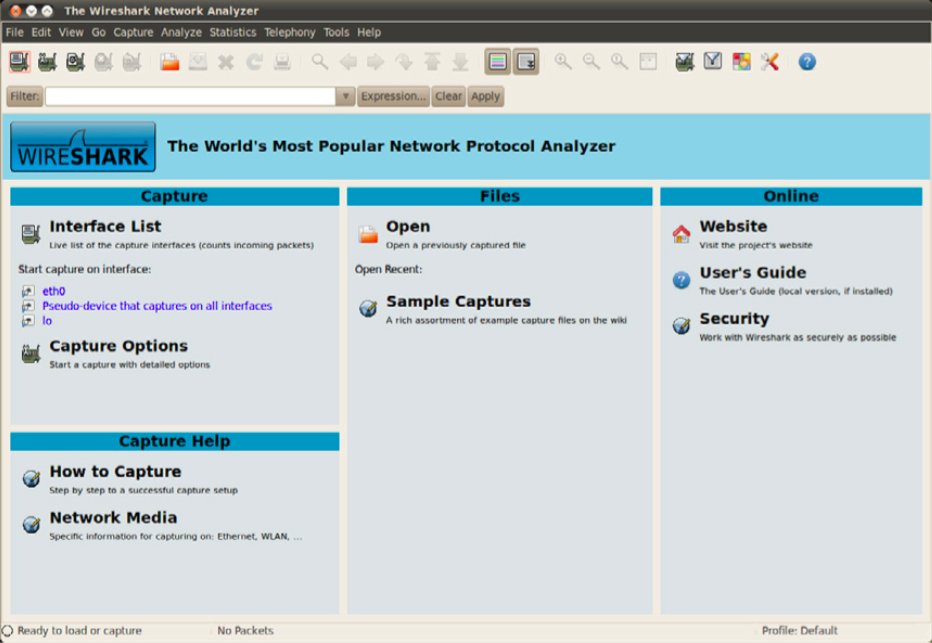
\includegraphics[scale=.3]{imgs/attack/wireshark.png}
	\caption{Wireshark sniffing tool}
	\label{wireshark_img}
\end{figure}

Per l'identificazione passiva, può essere utilizzato Wireshark, Figura \ref{wireshark_img}.\cite{wireshark} Wireshark cattura il traffico che attraversa qualsiasi rete in tempo reale e fornisce l'ispezione di centinaia di protocolli. È possibile inoltre specificare gli indirizzi IP di cui effettuare lo sniffing, così da limitare la raccolta di informazione ai possibili target.\\
Internet Control Message Protocol (ICMP) per individuare i target attivi in rete analizzando le loro response. Nel caso in cui il traffico ICMP sia bloccato, è spesso utilizzato il ping di TCP. Per entrambi i casi è utilizzato il tool di sicurezza Nmap\cite{nmap}.

\paragraph{Port Scanning}\mbox{}\\
Consiste nel fare \emph{probing} sul target in attesa di risposte sulle 65,536 porte TCP e/o UDP. Ottenere una response significa che dei servizi sono in esecuzione sulle porte associate e che potrebbero contenere debolezze che esporrebbero il target. Il tool di port-scanning più utilizzato è Nmap, che permette di effettuare scan TCP completando l'\emph{handshake}, o attraverso scan TCP SYN che utilizza solamente i messaggi iniziali di SYN e SYN ACK dell'\emph{handshake} TCP.\\
L'OSSTMM suggerisce che la scelta di quali delle 65,536 porte da analizzare è a discrezione dell'attaccante e dipende dal contesto.

\paragraph{Services Identification and System Identification}\mbox{}\\
Lo scopo di questi due moduli è di enumerare i servizi in esecuzione sulle porte TCP o UDP che hanno prodotto una response nella fase di port scanning, così come identificare il sistema operativo del target.\\
Entrambi i compiti sono svolti dal tool Nmap, attivando lo switch \textbf{-sV} che fornisce informazioni addizionali ad esempio il numero di versione, come è possibile verificare nella Figura \ref{nmap_sv_img}.\\
In questo caso il target utilizzato, \emph{webserver.domain.com}, fornisce informazioni quali il sistema operativo in quanto esposte dal server web Apache. Un attaccante userebbe le informazioni ottenute per verificare la presenza di falle nelle specifiche versioni dei servizi, per poi preparare un attacco.
\begin{figure}[hbtp]
	\centering
	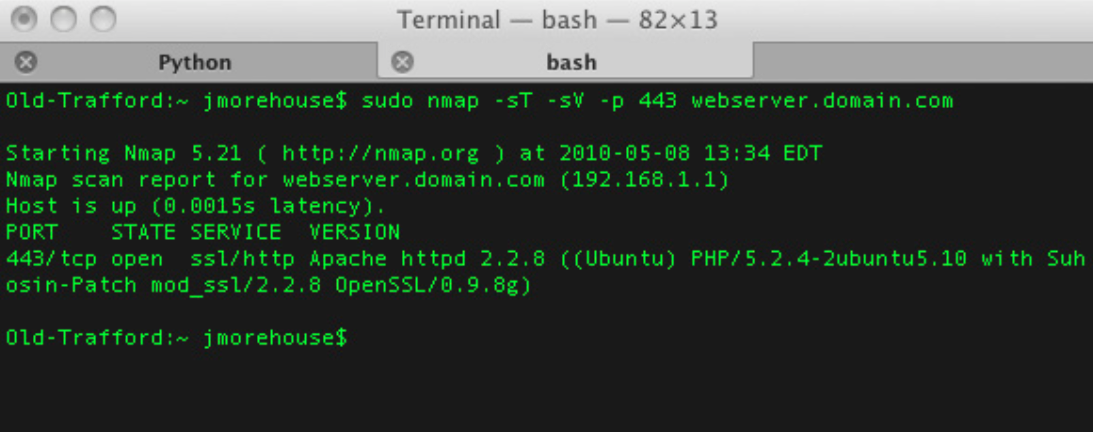
\includegraphics[scale=.3]{imgs/attack/nmap_sv.png}
	\caption{Nmap version detection ouput}
	\label{nmap_sv_img}
\end{figure}

\paragraph{Vulnerability Research and Verification}\mbox{}\\
Una volta noti sistema operativo e servizi in esecuzione con relative versioni si passa alla ricerca  e verifica di vulnerabilità tramite testing manuale ed automatizzato.\\
Un tool comunemente utilizzato per effettuare tale scan è Nessus \cite{nessus}, sviluppato dalla Tenable Network Security, mostrato in Figura \ref{nessus_img}. Sebbene Nessus sia ottimo per eseguire scanning automatizzato per determinare debolezze come una versione non aggiornata di Apache, il testing manuale dovrebbe coadiuvare quello automatizzato per individuare debolezze che potenzialmente potrebbero essere trascurate.\\
\begin{figure}[hbtp]
	\centering
	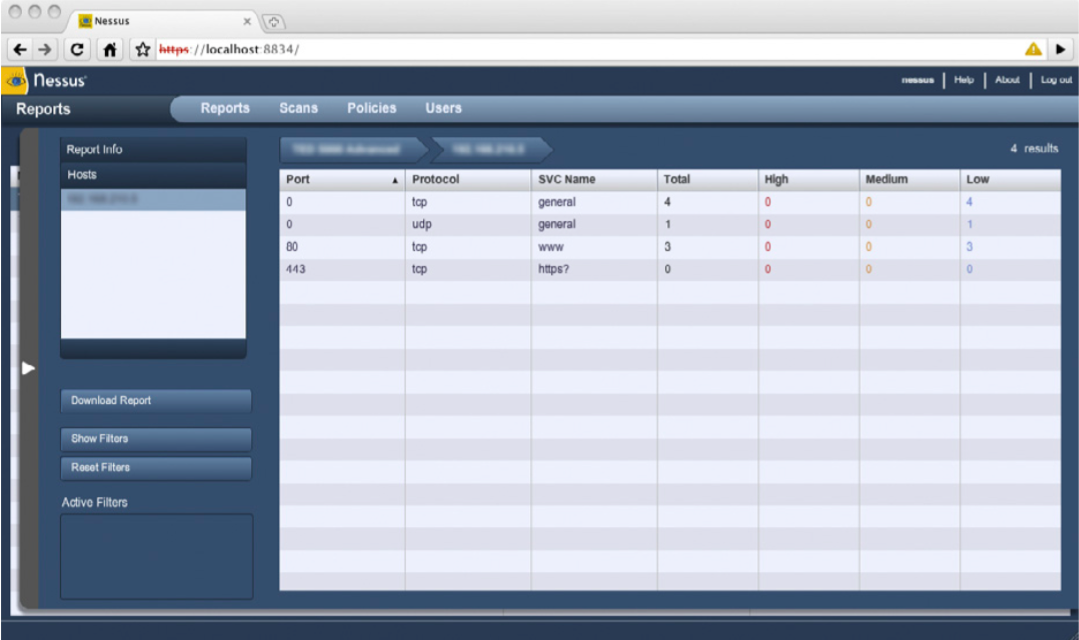
\includegraphics[scale=.3]{imgs/attack/nessus.png}
	\caption{Interfaccia web di Nessus}
	\label{nessus_img}
\end{figure}
L'OSSTMM consiglia che il testing automatizzato venga effettuato da almeno due scanner, seguito poi da una verifica manuale. Le tecniche utilizzate per la verifica manuale di vulnerabilità variano molto in funzione della vulnerabilità che si sta cercando, come ad esempio l'uso di Telnet per osservare la versione di uno specifico servizio connettendocisi, o l'utilizzo di un client FTP per connettersi ad un server FTP anonimo.\\
Nel processo di attacco a smart meter, la fase in esame è un passo critico in quanto fornisce i potenziali punti d'ingresso nello smart meter che potrebbero essere sfruttati nel modulo che segue.

\paragraph{Internet Application Testing}\mbox{}\\
Spesso, gli scanner di vulnerabilità non includono la possibilità di eseguire identificazione di vulnerabilità e verifica per Web application.\\
Con l'aumentare delle misure di sicurezza adottate dai produttori di sistemi all'interno del proprio ciclo di sviluppo, il numero di servizi in esecuzione a disposizione di attaccanti si è man mano ridotto. Ciò ha portato questi ultimi a concentrarsi sulle web application in esecuzione sui dispositivi target. Nel caso degli smart meter, tali applicazioni consentono al consumatore di visualizzare o configurare le informazioni di utilizzo, o permettono ai tecnici di configurare il dispositivo. Lo scopo di questo modulo è lo stesso del precedente, ma in un ambiente differente.\\
Effettuare identificazione e verifica di vulnerabilità su web application è significativamente più complesso che eseguire lo stesso test su servizi in esecuzione. Questo è il risultato del livello di personalizzazione trovato in ogni web application: è raro il caso che una web application sia esattamente come un'altra, ed anche nel caso di due \emph{webapp} identiche trovate in esecuzione, la loro infrastruttura di backend potrebbe differire. Per questo il testing manuale gioca un ruolo significativo e i tool a supporto di tale operazione sono molteplici. L' Open Web Application Security Project (OWASP) ha sviluppato una guida al testing per le web application, disponibile a questo indirizzo \url{https://www.owasp.org/index.php/Category:OWASP_Testing_Project}.

\paragraph{Password Cracking}\mbox{}\\
Questo modulo consiste nell'individuazione delle credenziali valide di un servizio in esecuzione o di una web application. Il testing può essere effettuato sia a partire da una lista precompilata di password, noto come attacco basato su dizionario, che provando ogni possibile combinazione di un certo alfabeto di caratteri, noto come attacco brute force.\\
Quando si esegue password cracking, è bene tenere a mente che molti servizi e web application implementano un servizio di blocco temporaneo o permanente, che disabilita un account se si verificano troppi tentativi di accesso con password invalide durante un determinato periodo di tempo.\\
Un tool comunemente utilizzato nell'ambito del password cracking, che supporti sia attacchi con dizionario che brute force, è Cain \& Abel \cite{cainabel}, mostrato in Figura \ref{cainabel_img}.\\
\begin{figure}[hbtp]
	\centering
	\includegraphics[scale=.3]{imgs/attack/cainabel.png}
	\caption{Il tool di password cracking Cain \& Abel}
	\label{cainabel_img}
\end{figure}
Il password cracking ha un ruolo fondamentale nell'attacco ad uno smart meter quando ci si trova davanti ad un prompt di autenticazione. Se un attaccante riesce ad ottenere le credenziali di uno smart meter, egli può istantaneamente avere accesso al dispositivo.

\paragraph{Denial of Service Testing}\mbox{}\\
Il modulo di Denial of Service si occupa di identificare i punti deboli che potrebbero essere del device stesso o all'interno dell'infrastruttura sottostante. Tale operazione potrebbe coinvolgere l'utilizzo degli strumenti precedentemente descritti, Wireshark e Nmap. Ad esempio, Wireshark potrebbe essere utilizzato per determinare i regolari pattern di traffico da e verso lo smart meter. Nmap invece potrebbe essere utilizzato per incrementare gradualmente il traffico verso lo smart meter nell'intento di sovraccaricare il dispositivo o la sua infrastruttura.\\
Se l'obiettivo dell'attaccante è semplicemente di negare il servizio ad uno smart meter, sarebbe molto semplice condurre un attacco del genere se comparato con attacchi che mirano alla compromissione della confidenzialità e/o integrità dello smart meter.

\paragraph{Exploit Testing}\mbox{}\\
Tutti i moduli descritti fin'ora gettano le basi per l'esecuzione dell'exploit testing. L'exploit testing punta ad utilizzare le vulnerabilità identificate per compromettere lo smart meter. Esempio di exploit testing includono l'utilizzo di codice per sfruttare un buffer overflow in un servizio in esecuzione o utilizzando SQL injection per accedere ad una shell di comando attraverso una falla nella validazione di un input all'interno di una web application.\\
Metasploit è un exploit tool disponibile gratuitamente che offre ai tester di sicurezza e agli attaccanti un considerevole numero di \emph{vulnerability exploit} e \emph{payload} \cite{metasploit}.
\begin{figure}[hbtp]
	\centering
	\includegraphics[scale=.3]{imgs/attack/metasploit.png}
	\caption{Il tool di vulnerability exploit Metasploit}
	\label{metasploit_img}
\end{figure}
Per un security tester, lo scopo finale è spesso quello di compromettere il target, laddove per un attaccante, la sola compromissione dello smart meter possa essere un altro passo nella propria metodologia personale di raggiungere l'obiettivo preposto.

%%%%%%%%%%%%%%%%%%%%%%%%%%%%%%%%%%%%%%%%%%%%%%%%%%%%%%%%%%%%%%%%%%%%%%%%%%%%%%%%%

\section{False Data Injection}
Nelle moderne Smart Grid, la rete elettrica tradizionale è potenziata dai più recenti progressi nei campi del sensing, della misurazione e dei dispositivi di controllo con una comunicazione bidirezionale tra produttore e consumatore. La produzione di elettricità, la sua trasmissione, la distribuzione ed il consumo, scambiano informazioni sullo stato della griglia che vengono recapitate agli utenti del sistema, agli operatori ed ai dispositivi.\\
La stima dello stato ha una funzione chiave nella costruzione di modelli \emph{real-time} della rete elettrica nei centri di gestione dell'energia (EMC) \cite{monticelli}. Un modello \emph{real-time} è una rappresentazione matematica quasi statica delle attuali condizioni all'interno di una rete elettrica interconnessa. Questa rappresentazione matematica è solitamente ottenuta dai dati provenienti dalle misurazioni e dalla telemetria che avvengono a distanza di pochi secondi nel centro di controllo dell'energia (ECC). Modelli \emph{real-time} della rete possono essere utilizzati per fare scelte ottimali, rispettando vincoli tecnici come congestione delle linee di trasmissione, voltaggio e stabilità transiente. In pratica, sia economicamente che in termini di fattibilità, non è possibile misurare tutti i possibili stati nella rete; quindi, la stima dello stato è uno strumento utile per stimare tali quantità, a partire da un insieme limitato di misurazioni. Solitamente sono usati due tipi di informazione per la stima dello stato:
\begin{itemize}
	\item Dati analogici di sistemi come flussi Megavar sulle linee principali, il carico \emph{P} e \emph{Q} sui generatori e trasformatori, e i voltaggi dei bus di sistema;
	\item Lo stato on/off dei dispositivi di switch come interruttori di circuito, switch di disconnessione, e tap dei trasformatori che determinano la topologia di rete.
\end{itemize}
A causa dell'importanza della stima dello stato, gli effetti negativi dell'\emph{iniettare} misurazioni scorrette sono studiati in letteratura \cite{baddatainj}.  Le misurazioni scorrette possono avvenire a causa di anormalità di misura impreviste, o iniezioni dovute ad attacchi malevoli. Ad esempio, \cite{falsedatainj} è il lavoro pionieristico nello studio degli attacchi di \emph{bad data injection} che non possono essere rilevati (chiamati \emph{stealth attacks}), e mostra come un attaccante possa portare a compimento tali attacchi ``\emph{stealth}" falsificando le misure del flusso elettrico alle unità terminali remote (RTUs), manomettendo l'eterogenea rete di comunicazione o infiltrandosi all'interno del sistema della supervisione di controllo e dell'acquisizione dati (SCADA) attraverso la LAN dell'ufficio del centro di controllo. Si consideri che un sistema SCADA o un sistema di misurazione su larga area (WAMS) ottiene informazioni sulla rete elettrica (valori delle misure, stato degli interruttori, ecc.) a specifici tempi e luoghi. I centri di controllo usano le informazioni collezionate per scopi diversi, ad esempio la risoluzione di un problema di stima dello stato. In \cite{baddatainj2}, viene mostrata la fattibilità degli  attacchi di bad data injection non rilevabili, con l'obiettivo di manipolare i prezzi del mercato elettrico.
\begin{figure}[h]
	\centering
	\includegraphics[scale=.3]{imgs/attack/fourbuspowernet.png}
	\caption{Illustrazione di una rete elettrica a quattro bus, centro di controllo, varie funzioni principali (AGC, OPF, EMS), e l'operatore. G rappresenta un generatore, il punto nero rappresenta misurazioni attive sul flusso di corrente ed il triangolo sul bus rappresenta il carico della regione o città.}
	\label{fourbuspowernet_img}
\end{figure}

\subsection{Stima dello stato e Bad Data Injection}
I sistemi elettrici in generale consistono di tre sottosistemi: generazione, trasmissione e distribuzione. Le linee di trasmissione sono utilizzate per trasmettere la corrente elettrica generata ai consumatori. In teoria, la corrente complessiva trasmessa tra il bus \emph{i} ed il bus \emph{j} dipende dalla differenza di voltaggio tra i due bus, ed è funzione dell'impedenza tra questi bus. In genere, le linee di trasmissione hanno un alto rapporto reattanza/resistenza ($X/R$), e quindi l'impedenza di una trasmissione può essere approssimata con la sua reattanza. La corrente attiva trasmessa dal bus \emph{i} al bus \emph{j} può essere scritta come
\\
\\
\indent$P_{ij} = \frac{V_{i}V_{j}}{X_{ij}}sin(\theta_{i} - \theta_{j})$,
\\
\\
dove $V_{i}$ è la tensione, $\theta_{i}$ è l'angolo di fase del voltaggio nel bus \emph{i}, ed $X_{ij}$ è la reattanza della linea trasmissiva tra il bus \emph{i} ed il bus \emph{j}.\\
Negli studi del flusso di corrente DC (che in questo caso sta per linearità delle equazioni piuttosto che corrente diretta), solitamente si assume che le differenze di fase tra due bus siano piccole, e che le ampiezze dei voltaggi nei bus siano vicine all'unità (dopo essere state normalizzate). Per cui, un'ulteriore semplificazione porta ad una relazione lineare tra gli angoli di fase e la reattanza delle linee,
\\
\\
\indent$P_{ij} = \frac{\theta_{i}\theta_{j}}{X_{ij}}$.
\\
\\
Negli studi sui flussi di potenza, l'angolo di fase del voltaggio ($q_i$) del bus di riferimento è fissato e noto; quindi, solamente $n - 1$ angoli devono essere stimati. I vettori di stato sono definiti come $\textbf{x} = [\theta_1, \ldots, \theta_n]^T$, cioè il vettore degli $n$ angoli di fase dei bus $\theta_i, i = 1, \ldots, n$.\\
Il problema della stima dello stato consiste nello stimare gli $n$ angoli di fase $\theta_i$, osservando $m$ misure in tempo reale, denotate dal vettore $\textbf{z}$ al centro di controllo. Queste misure potrebbero essere sia di corrente attiva trasmessa dal bus $i$ al bus $j$, $P_{ij}$, sia di corrente attiva al bus $i$, $P_i$. La corrente attiva iniettata nel bus $i$ è la super composizione della corrente trasmessa tramite le linee connesse al bus $i$ come $P_i = \sum_j{P_{ij}}$. Il vettore delle osservazioni $\textbf{z}$ può essere descritto come $\textbf{z} = \textbf{h(x)} + \textbf{e}$, dove $\textbf{h(x)}$ è la relazione non lineare tra le misure $\textbf{z}$ e lo stato del sistema $\textbf{x}$, ed $\textbf{e} = [e_1, \ldots, e_m]^T$ è il vettore del rumore Gaussiano delle misure con matrice di covarianza $\Sigma_e$.\\
La matrice del Jacobiano $\textbf{H} \in {\rm I\!R}$ è definita come\\
\indent$\textbf{H}=\frac{\partial\textbf{h(x)}}{\partial\textbf{x}}|_{x=0}$.\\
Se la differenza di fase è piccola, il modello di approssimazione lineare della misura di corrente può essere descritto come\\
\indent Misura sotto Operazioni Normali: $\textbf{z} =  \textbf{Hx} + \textbf{e}$.\\
Da notare che $\textbf{H}$ è generalmente sconosciuta agli attaccanti ma nota all'ISO. Date le misure sul flusso di corrente, il vettore di stato stimato $\widehat{x}$ può essere computato come $\widehat{\textbf{x}} = (\textbf{H}^T\sum_e^{-1}\textbf{H})-1\textbf{H}^T\sum_e^{-1}\textbf{z}$.\\
La Figura \ref{fourbuspowernet_img} mostra il sistema di test a quattro bus della IEEE: ogni bus ha il corrispondente voltaggio ($V_q$) e l'angolo di fase ($\theta_q$); il centro di controllo invia i dati delle misurazioni ($z_{qr}$) ed in seguito lo stimatore di stato inferisce gli stati del sistema che possono essere utilizzati in differenti funzioni, come ad esempio il controllo della generazione automatico (AGC), il flusso di controllo ottimale (OPF), ed il sistema di gestione dell'energia (EMS). L'operatore effettua la decisione finale per il controllo dei generatori e la gestione del carico (per bilanciare la fornitura e la domanda).
\subsection{Bad Data Detection}
Nella stima dello stato di un sistema elettrico, i ``bad data" come ad esempio bias di misurazione, derive di misura o connessioni errate devono essere identificate. Con il \emph{bad data injection}, gli attaccanti possono iniettare dati all'interno del vettore di misure $r$ ed il sistema può essere descritto come\\
\indent Misura sotto Attacco non-Stealth: $\textbf{z}^\prime = \textbf{H}(\textbf{x}) + \textbf{b} + e$, $\textbf{a} = I\textbf{b}$.\\
Si definisce il vettore residuo $\textbf{r}$ come la differenza tra le qualità misurate ed i valori calcolati dagli stati stimati, precisamente, $\textbf{r} = \textbf{z} - \textbf{H}\widehat{\textbf{x}}$. La media e la covarianza del residuale sono rispettivamente $E(\textbf{r}) = 0$, e $cov(\textbf{r}) = I\sum_{\epsilon}$, dove $I = \textbf{I} - \textbf{M}$, ed $\textbf{M} = \textbf{H}(\textbf{H}^T\sum_e^{-1}\textbf{H})-1\textbf{H}^T\sum_e^{-1}$.\\
I minimi quadrati pesati dell'errore di misura $r^{T}\sum_{e}^{-1}r$ seguono la distribuzione del chi-quadro con $n - m$ gradi di libertà \cite{monticelli}. L'ipotesi a riguardo del rilevamento dei dati fasulli può essere espressa come, $\textbf{r}^T\sum_{e}^{-1}\textbf{r} \ggll \chi_{n-m}^{2},\zeta$, dove $\zeta$ è la probabilità della confidenza del rilevamento.\\
I residuali normalizzati, di tutte le misure, sono utilizzati per identificare i ``bad data". Se la misura corrispondente al maggior residuale normalizzato è maggiore di una soglia di identificazione fissata $\gamma$, \\
\indent $max_i(|\textbf{r}_i|/\sqrt{cov(\textbf{r})}) \geq \gamma$,\\
allora quella misura è considerata come un dato fasullo ed è eliminato dalla stima dello stato.
\subsection{Stealth Bad Data Injection}
Utilizzando lo schema di rilevamento discusso precedentemente, il centro di controllo può difendersi da attacchi \emph{naive} di data injection ed identificare la sorgente di dati corrotti. Questo tipo di attacchi sono chiamati \emph{non stealth}. Però, se un attaccante ha conoscenza della topologia \textbf{H}, può iniettare dati fasulli della forma $\textbf{H}\delta\textbf{x}$ nella misura $\textbf{r}$, più precisamente,\\
\indent Misura sotto Attacco Stealth: $\textbf{z}^\prime = \textbf{H}(\textbf{x} + \delta\textbf{x}) + e$.\\
In questo caso, il test dell'ipotesi fallirebbe il rilevamento dell'attaccante, ed il centro di controllo crederebbe che il vero stato sia $\textbf{x} + \delta\textbf{x}$. Questa è chiamata \emph{stealth bad data injection}. Un'assunzione critica per la fattibilità di questo tipo di attacchi è la disponibilità di informazione completa sulla topologia. Tale assunzione può essere rilassata dal punto di vista dell'attaccante.
\subsection{Meccanismo Difensivo}
La strategia difensiva presentata in \cite{baddatainjattackdef} si basa sull'analisi statistica online della sequenza di dati simultanea al controllo del ritardo di rilevamento e la probabilità di errore entro i livelli desiderati. I metodi di stima dello stato convenzionali \cite{convdef1}, \cite{convdef2} per la \emph{bad data detection} utilizzano le misure per bilanciare il tasso di falsi allarme o il rapporto dei rilevamenti persi. Invece, l'approccio presentato in \cite{baddatainjattackdef} punta a minimizzare il delay di rilevamento soggetto al vincolo sulla probabilità di errore.\\
Si rappresenti con $z_t$ il vettore di osservazioni $m$-dimensionale al tempo $t$. In assenza di un avversario, $z_t$ può essere modellato, per trattabilità, come una distribuzione Gaussiana multivariata a media zero $\mathcal{N}(0, \sum_z)$. Si assume che l'avversario sia inattivo inizialmente; ad un tempo casuale sconosciuto $t$, diventa attivo ed inietta dati malevoli. L'ipotesi binaria può essere formulata come $\mathcal{H}_0: \textbf{Z}_t \sim \mathcal{N}(0, \sum_t)$ ed $\mathcal{H}_1: \textbf{Z}_t \sim \mathcal{N}(\textbf{a}_t, \sum_z)$, dove $\textbf{a}_t = [a_{t,1}, a_{t,2}, \ldots, a_{t,m}]^T \in R^m$ è il vettore dei dati malevoli sconosciuti iniettati dall'attaccante al tempo $t$, ed $\sum_z$ è $\textbf{H}\sum_x\textbf{H}^T + \sum_e$. In altre parole, si vuole rilevare un cambiamento nella distribuzione da $\mathcal(N)(0, \sum_z)$ a $\mathcal(N)(\textbf{a}_t, \sum_z)$ ad un tempo non noto $t$ con $\textbf{a}_t$ sconosciuto.\\
Sia $T_h$ lo \emph{stopping time}, il tempo in cui viene rilevato il cambiamento. Se $T_h < \tau$, è un falso allarme. La lunghezza di esecuzione media (ARL) è $T_d = E[T_h - \tau]$. Basandosi sulla formulazione di Lorden \cite{lorden}, è possibile minimizzare il delay nel caso peggiore, che può essere descritto come $T_d = sup_{\tau \geq 1} E_{\tau}[T_h - \tau | T_d \geq \tau]$. Per computare il minimo $T_d$, l'algoritmo CUSUM di Page è la miglior tecnica per affrontare questo tipo di problemi \cite{lorden}. La maggior parte dei modelli basati su CUSUM assume la conoscenza perfetta delle funzioni di likelihood. Nella detection della bad data injection, i parametri della distribuzione $\mathcal{H}_1$ non possono essere completamente definiti a causa dei parametri degli attaccanti e del modello statistico che non sono noti. Per cui, bisogna progettare meccanismi per il più rapido rilevamento in presenza di parametri non noti.\\
Il CUSUM test adattivo è ricorsivo per sua natura. Ogni ricorsione comprende due step interfogliati:
\begin{itemize}
	\item test CUSUM multi-thread
	\item risolutore lineare di parametri non noti
\end{itemize}
Il CUSUM test multi-thread estende l'algoritmo di Page. Esso considera il tasso di likelihood di $m$ misure a tempo $t$ così da determinare il tempo di stop $T_h$, che può essere descritto come $T_h = Inf\lbrace t \geq 1 | S_t > h \rbrace$, in cui la soglia di rilevamento $h$ è una funzione del tasso di falso allarme (FAR), del tasso di rilevamenti persi (MDR), e la varianza del processo, con statistiche cumulative al tempo $t$: $S_t = max_{1\geq k \geq T_h}\sum_{t=k}^{T_h}$, con $L_t$ pari alla somma della funzione del tasso di likelihood per tutte le misure $(z_{t,j}, j \in \lbrace1, 2, \ldots, m\rbrace)$ al tempo $t$. È possibile esprimere $L_t(\textbf{Z}_t)$ come\\
\indent $\sum_{j=1}^{m}log\frac{f_1(z_{t,j})}{f_0(z_{t,j})}$,\\
dove $f_1(z_{t,j})$ e $f_0(z_{t,j})$ corrispondono alla distribuzione della $j$-esima osservazione al tempo $t$ sotto attacco. Al tempo $t$, la statistica cumulativa $S_t$ può essere risolta ricorsivamente come $max[0, S_{t-1} + L_t(\textbf{Z}_t)]$, dove $S_0 = 0$ quando $t = 0$. Il centro di controllo fa scattare un allarme quando l'accumulazione supera una determinata soglia $h$.\\
A causa di un modello statistico avversario sconosciuto, il test del tasso di likelihood generalizzato (GLRT) può essere utilizzato nell'algoritmo CUSUM di Page \cite{lorden}. L'idea è quella di applicare GLRT sostituendo il parametro sconosciuto secondo la stima a maximum likelihood. Quindi, l'espressione ricorsiva del CUSUM test non è più valida in quanto GLRT ha bisogno di computare ogni elemento non noto di ogni misurazione al tempo $t$ stimandolo dalle osservazioni fino al tempo corrente $t$. In altre parole, GLRT richiede la memorizazione delle osservazioni e l'esecuzione della stima ML dei parametri sconosciuti ad ogni punto temporale. Per cui, GLRT è troppo costoso computazionalmente da implementare in pratica per effettuare rilevamento veloce.\\
Per ridurre la complessità computazionale, è possibile applicare il test Rao \cite{lorden}, che è un modello di test asintoticamente equivalente a GLRT. Il Rao test computa le derivate rispetto al parametro non noto valutato in zero, e può essere implementato efficientemente. Inoltre, il Rao test non coinvolge la complessa computazione della stima a maximum likelihood.\\
\subsection{Strategia di attacco}
Gli attacchi stealth sono attuabili quando gli attaccanti hanno piena conoscenza della topologia. Una domanda importante che sorge spontanea è: \textit{se la topologia non è disponibile, può un attaccante effettuare comunque stealth bad data injection?} Sorprendentemente, \textit{si}. L'idea principale presentata in \cite{esmalifalak}, si basa su parametri del sistema variabili in un piccolo range dinamico, infatti, l'informazione sulla topologia è incorporata nelle correlazioni tra le misure di flusso di potenza. Siano $\textbf{z}(t)$ e $\textbf{x}(t)$ le misure ed i vettori di stato al tempo $t$, dove $\textbf{x}(t)$ è sconosciuto. Ad un certo tempo $t$, è impossibile inferire $\textbf{H}$ solamente a partire da $\textbf{z}(t)$. Comunque, con il passare del tempo, e la conoscenza delle proprietà stocastiche del processo casuale $\textbf{x}(t)$, si potrebbe essere in grado di inferire \textbf{H}.\\
Nei sistemi elettrici, le variabili di stato sono generalmente una funzione non lineare dei carichi \textbf{y} e della topologia \textbf{H: x = } \emph{f}(\textbf{y, H}). Mentre la topologia è nota per essere statica in un determinato periodo temporale, i carichi possono essere modellati come \textit{indipendentemente} variabili. Se tali variazioni sono sufficientemente piccole, \emph{f} può essere approssimata utilizzando $\textbf{x} = \textbf{Ay}$, dove \textbf{A} è la matrice dei coefficienti di primo ordine dell'espansione di Taylor in \textbf{y} ($\textbf{z = HAy + e}$).\\
Con \textbf{HA} ed \textbf{y}, è possibile portare a compimento l'attacco modificando i dati misurati come $\textbf{z}^\prime + \textbf{HA}\delta\textbf{y}$, dove $\delta\textbf{y}$ è scelto arbitrariamente.
Il vettore di stato è stimato come $\widehat{\textbf{x}} = (\textbf{H}^T\sum_e^{-1}\textbf{H})-1\textbf{H}^T\sum_e^{-1}\textbf{z}^\prime$. Sia $\delta\textbf{x} = A\delta\textbf{y}$. Siccome $r = \textbf{z}^\prime - \textbf{H}\wedge x = \textbf{z} + \textbf{H}(\widehat{\textbf{x}} + \delta\textbf{x}), E(\textbf{r}) = 0, cov(\textbf{r}) = (\textbf{I} - \textbf{M})\sum_e$. In altre parole, la media e la varianza di \textbf{r} sono le stesse del caso senza attaccanti. Quindi, utilizzando il metodo del residuale massimo, l'attacco non può essere rilevato.\\
Per inferire \textbf{HA} ed \textbf{y}, è possibile adottare la tecnica della \emph{linear independent component analysis} (ICA). La Linear ICA \cite{lica} è un metodo sviluppato di recente che ha lo scopo di trovare una rappresentazione lineare dei dati cosicché le componenti siano quanto più statisticamente indipendenti possibile. È un caso speciale della \emph{blind source separation}, formulata come segue.
\indent $\textbf{u} = \textbf{Gv}$,\\
con $\textbf{u} = [u_i, i = 1,2, \ldots, m]$ che è il vettore delle osservazioni degli $m$ segnali di monitoraggio, $\textbf{G} = [g_{ij}, i = 1, 2, \ldots,m, j = 1 ,2, \ldots, n]$ è la matrice di mixing non nota, e $v = [v_i, i = 1, 2, \ldots, n]$ è il vettore delle $n$ variabili indipendenti latenti.\\
Dato il modello e la realizzazione di \textbf{u}, ICA può inferire sia la matrice di mixing \textbf{G} che il vettore \textbf{v} calcolando in maniera adattiva il vettore dei pesi \textbf{w} che massimizza una misura di \emph{non Gaussianità} del $\textbf{w}^T\textbf{u}$ calcolato.\\
\begin{figure}[htbp]
	\centering
	\fbox{\begin{minipage}{15em}
			Input: \textbf{z} = data matrix
			\begin{enumerate}
				\item $\lbrack \textbf{G}$ and $\textbf{y} \rbrack$ = FastICA(\textbf{z})
				\item If max(\textbf{z} - \textbf{Gy})  $>$ $\epsilon$ then exit
				\item Generate $\delta$\textbf{y} $\sim N(0, \sigma^2)$
				\item $\textbf{z}^\prime$ = \textbf{z} + \textbf{G}(\textbf{y} + $\delta$\textbf{y})

			\end{enumerate}
			Output: false data $\textbf{z}^\prime$
		\end{minipage}
	}
	\caption{Stealth false data injection.}
	\label{algo1}
\end{figure}
L'algoritmo è mostrato in Figura \ref{algo1}: FastICA \cite{lica}, alla riga 1, è un algoritmo popolare ed efficiente per la ICA che iterativamente trova la direzione in cui il vettore dei pesi \textbf{w} massimizza la non Gaussianità della proiezione $\textbf{w}^T\textbf{z}$ per i dati \textbf{z}. \textbf{G} deve soddisfare $\textbf{w}^T\textbf{G} = \textbf{I}$, con \textbf{I} matrice identità. Le entrate di \textbf{G} minori di una certa soglia $\epsilon$ sono rimosse. Infine, il vettore di stato \textbf{y} può essere stimato da $\textbf{w}^T\textbf{z}$.\\
La riga 2 verifica che \textbf{z} segua un modello lineare. Se le assunzioni di linearità sono valide, $max(\textbf{z} - \textbf{Gy})$ dovrebbe essere piccolo.\\
La riga 3 genera un attacco random tramite una variabile casuale Gaussiana, ed è aggiunto alla variabile inferita \textbf{y} alla riga 4, risultando così in un attacco stealth che non può essere rilevato.


%%%%%%%%%%%%%%%%%%%%%%%%%%%%%%%%%%%%%%%%%%%%%%%%%%%%%%%%%%%%%%%%%%%%%%%%%%%%%%%%%
\section{Disconnect Attack}
Gli smart meter sono la parte più visibile della transizione verso la moderna Smart Grid. Questi sono tipicamente controllati ed interrogati attraverso comunicazioni wireless o su power-line: tali comunicazioni e possibilità di controllo remoto introducono potenziali fonti di attacco con conseguenze gravi per i consumatori ed i proprietari delle infrastrutture.\\
In particolare, lo switch di servizio e la possibilità di connessione/disconnessione remota (RCD) associata degli smart meter, ha colpito l'attenzione della comunità della sicurezza negli ultimi anni \cite{offswitch}, \cite{remotecontrol}, \cite{amithreats}. Un attacco RCD potrebbe causare un blackout diffuso su larga scala o addirittura la minaccia di compiere il suddetto attacco in cambio di soldi \cite{offswitch}. Questo tipo di attacco potrebbe potenzialmente danneggiare la rete elettrica o altri carichi elettrici causando deviazioni nel voltaggio o nella frequenza \cite{remotecontrol}. In tutti i casi, un attacco portato a termine avrebbe serie conseguenze politiche ed economiche.\\
Mentre le misure di sicurezza come la cifratura dei dati ed i sistemi di rilevamento delle intrusioni (IDS) offrono un certo livello di protezione per i sistemi AMI, essi non sono d'aiuto nel caso in cui un attaccante sia capace di compromettere il sistema e far eseguire comandi malevoli a centinaia di migliaia (o milioni) di dispositivi.\\
Le contromisure adottate, presenti in letteratura, fanno uso di ritardi casuali per l'esecuzione dei comandi RCD rendendo così la Smart Grid più resistente:\\
\begin{enumerate}
	\item Prevenendo rapidi cambiamenti nel carico che potrebbero destabilizzare il sistema elettrico;
	\item Dando il tempo di rilevare e fermare un attacco in corso.
\end{enumerate}
Tali meccanismi di ritardo sono tecnicamente fattibili: alcuni meter supportano un ritardo configurabile prima di rispristinare il servizio dopo un guasto \cite{disconnectfaqs}.
\subsection{Modellare attacchi di Remote Disconnect su AMI}
Si descrivono di seguito i modelli del sistema e degli attaccanti utilizzati per studiare le contromisure di \emph{time delay} per attacchi RCD.
\subsubsection{Modello del sistema}
Si consideri il sistema semplificato di una Smart Grid, in Figura \ref{simplesg_img}, in cui una compagnia utilizza un'unità AMI per controllare un insieme di smart meter a casa dei propri clienti. La comunicazione tra l'unità ed il meter è instradata da più \emph{data concentrator unit} (DCU) intermedi, posizionati in \emph{neighborhood area networks} (NANs). L'unità può effettuare richieste di disconnessione, tramite un DCU, di qualunque meter. Il modello permette di astrarre da protocolli, tecnologie di comunicazione e funzionalità di sicurezza disponibili.\\
\begin{figure}[h]
	\centering
	\includegraphics[scale=.3]{imgs/attack/simpleSG.png}
	\caption{Ambiente semplificato. Smart Grid con AMI, sistema di gestione guasti ed un attaccante che sta inviando comandi di disconnessione da remoto ai meter.}
	\label{simplesg_img}
\end{figure}
Il modello del sistema include un \emph{outage management system} (OMS), presso la compagnia, raggiungibile dai clienti tramite telefono o internet. Tale OMS consente alla compagnia di aggregare ed analizzare i report degli utenti.
\subsubsection{Modello dell'attaccante}
Si consideri un attaccante con due scopi possibili:
\begin{enumerate}
	\item Denial-of-electrical-service per i clienti di un'azienda durante un determinato periodo di tempo;
	\item Disturbo fisico della frequenza della rete elettrica attraverso l'eliminazione del carico.
\end{enumerate}
L'impatto del primo attacco, un attacco di disconnessione su vasta scala in una importante città, può essere devastante ed è discusso in dettaglio in \cite{offswitch}. Oltre questo scenario da caso pessimo, gli attacchi RCD su scala minore (ad esempio a livello del vicinato) possono comunque avere serie ripercussioni, ed essere meno impegnativi per gli attaccanti \cite{amithreats}. Il secondo attacco, la connessione/disconnessione mirata di meter per modificare i parametri del sistema elettrico, discusso in \cite{remotecontrol}. Tale attacco richiederebbe un alto livello di conoscenza del sistema così come un alto numero di dispositivi compromessi.\\
Si modella un attaccante forte per entrambi gli scenari come segue: si assuma che l'attaccante abbia la conoscenza esatta dell'infrastruttura della compagnia (inclusa la topologia di rete, le specifiche degli smart meter e le strategie di controllo) e delle contromisure impiegate dal sistema. L'attaccante può trasmettere messaggi di disconnessione ad ogni meter e tali comandi sono accettati come autentici. Questa astrazione tiene conto di un vasto numero di vettori d'attacco possibili; ad esempio, la compromissione della master key dell'unità AMI, lo sfruttamento di una falla di un protocollo debole e attacchi dall'interno da parte di un operatore AMI. L'attaccante può prevenire la trasmissione di messaggi sul canale di comunicazione primario, se necessario (ad esempio, facendo uso di jammer). L'attaccante è limitato all'interazione con l'unità, DCU e smart meter, inoltre, non può attaccare direttamente l'OMS, la compagnia o canali di comunicazione secondari.
\subsection{Contromisura Delayed Disconnect}
Molte sono le contromisure a disposizione delle compagnie preoccupate per attacchi RCD. Autenticazione e schemi di gestione delle chiavi ben progettati sono componenti essenziali della soluzione, ma in assenza di potenti meccanismi di rilevamento, c'è poco da poter fare nel caso in cui un attaccante ottenga accesso al sistema. I sistemi di \emph{intrusion detection} (IDS) sono un'area di ricerca molto attiva, ma un attaccante potrebbe essere capace di eludere o disabilitare il sistema.\\
Per tale ragione, \cite{delay} concentra la sua attenzione su un altro tipo di contromisura - un delay a tempo casuale per tutte le operazioni RCD. Questo delay dovrebbe essere implementato in ogni smart meter, e la configurazione dei parametri di delay dovrebbe richiedere la presenza fisica per prevenire che un attaccante li modifichi da remoto. Anche se l'IDS o le misure di autenticazione fallissero, questo meccanismo di delay renderebbe la Smart Grid più resistente prevenendo rapidi cambiamenti nel carico e fornendo il tempo necessario al rilevamento di un attacco in corso così da poterlo fermare.\\
Le specifiche dei meccanismi di rilevamento e rispristino dipendono da molti fattori e dal sistema della compagnia. In \cite{delay} è analizzato un meccanismo di rilevamento che comprende il processo di gestione dei guasti della società, come mostrato in Figura \ref{simplesg_img}.\\
Se un attaccante disconnette con successo lo smart meter di un cliente, questo sarà in grado di contattare la compagnia e riferire la perdita di corrente entro un intervallo di tempo ragionevole. Se l'attaccante colpisce un gran numero di clienti, l'OMS della compagnia inizia a ricevere un alto numero di comunicazioni, che innescano un'investigazione. Una volta che l'investigazione stabilisce che i guasti erano di origine malevola, la compagnia può reagire. Si assume che la compagnia sia in grado di far scattare da remoto una modalità \textit{fail-safe}, che cancella tutte le richieste di disconnessione dei meter in sospeso. Questo \emph{trigger} può essere inviato attraverso il canale di comunicazione primario, o nel caso questo sia in controllo dell'attaccante, su un canale secondario. Una possibilità potrebbe essere quella di utilizzare radio secondarie o riconfigurabili \cite{radio}. Un'altra è l'attivazione manuale da parte dell'utente.\\
Ed è proprio la presenza di umani nella rete che rende questa contromisura impegnativa per un attaccante - a patto che il periodo di delay sia lungo abbastanza da far terminare il processo di rilevamento/intervento. Questo fa nascere spontanea la domanda su quanto il delay colpisca le operazioni giornaliere della compagnia, che fa uso di RCD per varie applicazioni.
\subsection{Impatto del delay sui tempi di operazioni RCD}
Si discutono quattro casi d'uso per compagnie RCD (raggruppati in tabella \ref{tab:usecases}) e stimata la loro sensibilità ai time delay. Usando queste stime, sono sviluppate contromisure che migliorano la resistenza del sistema con basso impatto sulle operazioni giornaliere.\\
\subsubsection{Routing Service Switching}
Quando un cliente si trasferisce, la compagnia necessita di fare un \emph{routine service toggling}. Le aziende possono ridurre significativamente i costi operazionali effettuando tali compiti da remoto, piuttosto che inviare tecnici sul luogo. Mentre lo switch del servizio da remoto è portato a termine in minuti \cite{toggle1}, \cite{toggle2}, non è un'operazione particolarmente \emph{time-critical}. Se un'abitazione è stata sgomberata, avrà una richiesta energetica residuale molto bassa. Inoltre, mentre alla comagnia è noto un periodo di trasferimento giorni prima, non lo è l'ora esatta del giorno. Per cui, è ragionevole aspettarsi una finestra RCD di alcune ore.
\subsubsection{Clienti non paganti}
Senza la possibilità di disconnessione da remoto, l'azienda deve disporre di personale addetto alla disconnessione dei clienti non paganti. A volte, questi tecnici sono minacciati quando provano ad accedere al meter. Quindi la disconnessione remota fornisce un guadagno assicurato, così come un beneficio di sicurezza importante. Se un cliente che dispone di uno smart meter \emph{RCD-enabled} non paga le sue bollette, l'azienda può disporre di un ``hard'' switch-off, o di un ``soft'' switch. Così come per il routine service switching, anche questo caso d'uso non è particolarmente time-critical. Senza RCD, potrebbe tranquillamente richiedere ore o addirittura giorni identificare un cliente non pagante, schedulare la disconnessione manuale, e spedire un tecnico in quella particolare area. Per cui questo caso d'uso dovrebbe consentire una finestra RCD di qualche ora.
\begin{table}[hbtp]
	\centering
	\begin{adjustbox}{max width=\textwidth}
		\begin{tabular}{|l|l|l|l|l|}
			\hline
			Num. & Caso d'uso & Beneficio Aziendale & Requisito Temporale & Alternative \\ \hline
			1 & Routine service switching & Risparmi di costi & Ore & Switch Manuale \\ \hline
			2 & Clienti non paganti & Sicurezza del dipendente, garanzia di guadagno & Ore & Switch Manuale\\ \hline
			3 & Limitazione della domanda & Gestione demand-side & Minuti - Ore & Prezzo Dinamico\\ \hline
			4 & Cancellazione dle carico & Controllo del carico a basso livello & Minuti - Ore & Interruttori delle sottostazioni\\ \hline
		\end{tabular}
	\end{adjustbox}
	\caption{Casi d'uso per Smart Meter Remote Connect/Disconnect}
	\label{tab:usecases}
\end{table}
\subsubsection{Limitazione della domanda}
Molti meter supportano una modalità \emph{demand limiting}, che penalizza clienti (sia attraverso la disconnessione o forzando un prezzo più alto dell'elettricità) che eccedono un livello massimo predefinito. È importante tenere presente che la domanda è definita come il carico del cliente in media su un determinato periodo di tempo \cite{demand}. In pratica, questo intervallo temporale sarebbe tra i 5 ed i 30 minuti. Se uno smart meter rileva una violazione del limite della domanda, dovrebbe essere capace di eseguire la conseguenza appropriata nel prossimo intervallo. Comunque, delay più lunghi prima dello \emph{shutoff} potrebbero verificarsi in alcuni casi, come ad esempio un governo che imponga un limite obbligatorio per abitazione. In uno scenario del genere, la disconnessione del meter agisce da deterrente più che da meccanismo di response real-time.
\subsubsection{Cancellazione del carico}
Sebbene le compagnie siano sempre state capaci di eliminare il carico aprendo gli interrutori di circuito, la presenza di smart meter RCD-enabled consente di avere una response più precisa. Il tempo d'esecuzione richiesto per la cancellazione del carico differisce in funzione dell'applicazione. Ad esempio, in situazioni di emergenza la compagnia deve essere in grado di eliminare il carico in real-time. In un sistema con carenze di forniture che necessita di andare in blackout, gli smart meter RCD-enabled consentono un preciso controllo del carico con vincoli temporali meno stringenti.
\subsection{Progettazione delle contromisure di delay}
Introdurre delay prima dell'esecuzione di comandi RCD dovrebbe avere un basso impatto sui casi d'uso visti nella sezione precedente, finché il delay è tenuto al di sotto di una certa soglia. Questo delay massimo è indicato da $d_{max}$, che è variabile dalle decine di minuti alle 2 ore circa, in base agli scenari. Si vede ora come usare questo periodo di delay per migliorare la capacità di recupero della Smart Grid.\\
\subsubsection{Contromisura Delay: il modello}
Si consideri una compagnia con $n$ RCD-enabled smart meter. Lo scopo dell'azienda è di minimizzare il numero totale di meter disconnessi progettando una distribuzione appropriata dei delay temporali su $[0, d_{max}]$. Come anticipato nel Modello del sistema, si considera un processo di rilevamento che coinvolge un sistema di gestione delle interruzioni, che riceve comunicazioni sui guasti da parte degli utenti. \cite{delay} sviluppa due modelli per il processo di rilevamento da parte dell'OMS, con differenti livelli di astrazione: un modello semplificato per la valutazione analitica, ed un altro più dettagliato da utilizzare all'interno di simulazioni.\\
Nel modello semplificato si assume che l'azienda sia capace di rilevare e fermare un attacco in corso entro $d$ minuti $(d < d_{max})$ una volta che $\tau$ meter siano stati disconnessi in una determinata finestra temporale. In questo modello, $d$ include il tempo necessario affinché i clienti interessati (disconnessi) possano segnalare il guasto, ed il tempo necessario alla compagnia per investigare e concludere che sta avvenendo un attacco, ed inviare comandi che fermino tutte le connessioni in maniera \emph{fail-safe}.\\
Nel modello più dettagliato, si assume che l'attacco sia rilevato una volta che siano state ricevute $\tau^\prime$ segnalazioni di guasto da parte dei clienti tramite l'OMS durante un periodo temporale (i tempi di segnalazione individuali sono campionati da una specifica distribuzione).
Quando questa condizione è verificata, l'azienda ha tempo aggiuntivo, $d^\prime$, per investigare prima di inviare comandi \emph{fail-safe}. In ogni caso, il valore di $\tau$ $(o$ $\tau^\prime)$ dovrebbe corrispondere ad una piccola frazione del numero totale di meter, ma deve essere grande abbastanza da escludere la maggior parte dei guasti non relativi alla sicurezza. Il tempo di risposta $d$ $(o$ $d^\prime)$ dovrebbe essere circa dello stesso ordine di $d_{max}$. L'intervallo temporale impostato per il rilevamento in accordo alla finestra temporale dell'obiettivo dell'attaccante, che si assume essere nell'ordine delle ore.
\subsubsection{Meccanismi di delay}
Le performance della contromisura RCD time delay dipende dalla distribuzione del delay, che deve essere progettata contro un attaccante che può selezionare il numero di meter da colpire e pianificare quando inviare i comandi di disconnessione. Si considerino ora, tre distribuzioni di delay: uniforme, Bernoulli e geometrica. Si sviluppano i limiti analitici per il numero di meter che un attaccante può disconnettere con successo seguendo una sua strategia ottimale. La Figura \ref{distributions_img} mostra le funzioni di probabilità densità/massa dei tre meccanismi.
\begin{figure}[hbtp]
	\centering
	\includegraphics[scale=.45]{imgs/attack/distributions.png}
	\caption{Meccanismi di delay RCD.}
	\label{distributions_img}
\end{figure}
\paragraph{Delay Uniforme.} Secondo questo meccanismo di delay molto basico, una volta che un meter riceve un comando di disconnessione autenticato, esso seleziona un back-off di delay casuale uniformemente da $[0, d_{max}]$. Ogni meter seleziona il suo delay di back-off indipendentemente e si disconnette dopo tale tempo.\\
Si esamini il momento in cui $\tau$ meter si sono appena disconnessi. Secondo il modello di rilevamento e notifica, l'azienda sarebbe in grado di fermare l'attacco entro altri $d$ minuti, annullando tutti i comandi di disconnessione che sono ancora in corso. Durante questi $d$ minuti, l'attaccante può continuare a disconnettere $nd/d_{max}$ meter aggiuntivi in media, assumendo che un attaccante abbia già inviato i comandi di disconnessione a tutti i meter. Siccome non c'è miglior strategia di attacco, questo fornisce un limite superiore al numero totale di meter disconnessi pari a $\tau + dn/d_{max}$, che cresce linearmente con $n$ dato $d/d_{max}$ costante.
\paragraph{Delay Bernoulli.} Una distribuzione alternativa per ridurre il numero di meter disconnessi è la distribuzione di Bernoulli. In pratica, ogni meter lancia una moneta truccata per scegliere tra due possibili intervalli, ognuno di almeno 10 secondi per evitare problemi di stabilità. In particolare, con probabilità $\alpha$ (parametro di sistema), il meter si disconnette quasi immediatamente, Altrimenti, esso pospone la sua disconnessione verso la fine del periodo consentito $(delay \approx d_{max})$. L'intuizione alla base è semplice: se sono attaccati un gran numero di meter, quelli che si disconnettono quasi immediatamente innescherebbero il rilevamento da parte dell'OMS, che a sua volta ferma l'attacco in corso per la maggior parte dei meter che pospongono la disconnessione.\\
In questo caso la miglior strategia per un attaccante è di non inviare comandi di disconnessione a tutti gli $n$ meter in un solo colpo: continuando ad utilizzare questa strategia consentirebbe alla compagnia di impostare $\alpha$ ad un valore molto basso così da ridurre il numero di meter disconnessi. Invece, un attaccante può massimizzare il numero di meter disconnessi lanciando un attacco \emph{two-batch}: l'attaccante sceglie il numero totale di meter in un primo gruppo così che il sottoinsieme di meter disconnessi immediatamente non faccia scattare la notifica. Nel momento in cui il sottoinsieme di meter del primo gruppo che sceglie di posporre inizia a disconnettersi (e notificherà presto all'azienda), l'attaccante invia i comandi a tutti gli altri meter. Sotto un attacco del genere, tutti i meter nel primo gruppo e, ci si aspetta, un sottoinsieme di una frazione $\alpha$ dei meter nel secondo gruppo si sarebbero disconnessi prima che i comandi di disconnessione in attesa siano annullati. Sommando questi due termini otteniamo un limite superiore al numero totale di meter disconnessi pari a $\tau/\alpha + (n - \tau/\alpha)\alpha$. L'azienda potrebbe scegliere strategicamente $\alpha = \sqrt{\tau/n}$ per minimizzare il limite a $2\sqrt{\tau n} - \tau$, che cresce in maniera sublineare in $n$.
\paragraph{Delay Geometrico.} Se il delay RCD massimo $d_{max}$ è poche volte maggiore di $d$, la compagnia può ridurre ulteriormente il numero di meter disconnessi applicando una distribuzione geometrica sui periodi di delay consentiti. Sia $k = [d_{max}/d]$. Con questo meccanismo di delay, un meter sceglierà tra $k$ possibili intervalli, con l'$i$-esimo $(i = 1, \ldots, k)$ intervallo di delay di durata circa $(i - 1)d/d_{max}$ e scelto con probabilità $(\beta^i - \beta^{i-1})/(\beta^k - 1)$. In questo caso, $\beta$ è un parametro di sistema che può essere ottimizzato in accordo a $k$ ed altri parametri (ad esempio $n$ e $\tau$). Si noti che quando $k = 2$, l'ottimizzazione di $\beta$ degenererebbe il meccanismo di delay geometrico nel meccanismo di delay Bernoulliano.\\
Utilizzando questa distribuzione geometrica ed il modello definito in precedenza, a prescindere dalla strategia adottata dall'attaccante, in media meno di $\tau(1+\beta) + (n - \tau)(\beta - 1)/(\beta^k - 1)$ meter sarebbero disconnessi. Il primo termine limita il numero di meter a cui è stato inviato il comando di disconnessione prima che $\tau$ meter siano disconnessi, ed il secondo termine limita il numero di meter a cui è stato inviato il comando di disconnessione dopo di ciò. Con la costante $\beta$, il primo termine cresce linearmente con $\tau$, che è una piccola frazione di $n$, ed il secondo termine decade geometricamente con $k$, che sarà anch'esso una piccola frazione di $n$, anche per piccoli valori di $k$.
\paragraph{Riepilogo.}
\begin{figure}[hbtp]
	\centering
	\includegraphics[scale=.5]{imgs/attack/dist_perf.png}
	\caption{Riepilogo dell'analisi con un setting d'esempio di $d = 10$ min, $d_{max} = 60$ min, $\tau = 1000$ ed $n = 600.000$.}
	\label{dist_perf_img}
\end{figure}
La Figura \ref{dist_perf_img} riassume i risultati analitici per i tre meccanismi di delay. Per ognuno di essi, il numero di meter disconnessi cresce ad un tasso asintotico differente rispetto ad $n$. Come illustrato nel setting d'esempio, secondo il meccanismo di delay geometrico, fin quando $d_{max}$ è poche volte (ad esempio, $6\times$) maggiore di $d$, il numero di meter disconnessi sarà piccolo $(< 1\%$ di $n)$. In confronto, secondo il meccanismo di delay uniforme, un numero significativamente maggiore di meter $(> 10\%$ di $n)$ sarebbe disconnesso. Per il meccanismo di delay di Bernoulli, il numero di meter disconnessi è nell'ordine di $\sqrt{\tau n}$, quindi dipende altamente dalla soglia di rilevamento $\tau$. Quando $\tau$ è circa lo $0.2\%$ di $n$ (come nei setting d'esempio), il numero di meter disconnessi può comunque raggiungere circa l'$8\%$ di $n$. Un confronto di questi tre meccanismi di delay suggerisce:
\begin{enumerate}
	\item Se possibile, un'azienda dovrebbe rendere $d_{max}$ svariate volte maggiore di $d$, ed utilizzare il meccanismo di delay geometrico;
	\item Altrimenti, se $\lceil d_{max}/d \rceil = 2$ ed il meccanismo di distribuzione geometrico degenera al Bernoulliano, la compagnia deve portare la sua soglia di rilevamento $\tau$ al valore minore possibile per favorire la propria capacità di recupero sotto attacchi RCD.
\end{enumerate}
%%%%%%%%%%%%%%%%%%%%%%%%%%%%%%%%%%%%%%%%%%%%%%%%%%%%%%%%%%%%%%%%%%%%%%%%%%%%%%%%%
%\section{Replay Attack}
%%%%%%%%%%%%%%%%%%%%%%%%%%%%%%%%%%%%%%%%%%%%%%%%%%%%%%%%%%%%%%%%%%%%%%%%%%%%%%%%%
\section{Jamming}
L'infrastruttura di comunicazione svolge un ruolo predominante nelle Smart Grid. Si occupa principalmente di broadcast real-time del prezzo della corrente, di riportare i consumi energetici e di monitorare lo stato del sistema. Grazie allo scambio di informazioni in tempo reale un utente è in grado di determinare il proprio consumo energetico ottimale.\newline
Così come i vantaggi, l'infrastruttura di comunicazione presenta alcune vulnerabilità. In questa sezione, si analizza in dettaglio una strategia di attacco che manipola il mercato elettrico utilizzando la tecnica del \emph{Jamming}. Questo attacco causa cambiamenti nei consumi energetici e tende quindi a destabilizzare le power grid (vedi Figura \ref{fig:jm}).
\begin{figure}[h]
	\centering
	\includegraphics[scale=0.320]{imgs/attack/jm.png}
	\caption{Un'illustrazione della manipolazione del mercato attraverso il Jamming} \label{fig:jm}
\end{figure}\\
Si assume che è utilizzato un sistema di comunicazione wireless, come WiMAX, per effettuare il broadcast delle informazioni relative ai prezzi. Un attaccante, utilizzando un jammer molto potente in un'area abbastanza vasta, disturba l'invio real-time dei prezzi\cite{jamming}. Si assume che ogni consumer continua a far riferimento al vecchio prezzo in quanto le informazioni aggiornate sul prezzo non arrivano a destinazione. L'attaccante continua a fare jamming fin quando non c'è una variazione reale sul prezzo. Una volta ricevuto il nuovo prezzo, gli utenti coinvolti modificheranno e/o si adegueranno, causandone una diminuzione o un incremento, facile da predire. In questo modo un attaccante può cambiare il prezzo della corrente quando e nella direzione in cui vuole.
%\subsection{Modello del sistema}
%Si considera una power grid con $N$ bus. Ogni bus è connesso ad un generatore elettrico. Sul bus \emph{n}, la corrente generata è denotata da \emph{$G_{n}$} e il costo unitario per la generazione è indicato con \emph{$C_{n}$}. Si assume vi siano \emph{M} utenti su ogni bus. L'$m$-esimo utente sul bus $n$ ha un consumo energetico $d_{nm}(t)$ nello slot temporale \emph{t}. Il consumo energetico totale sul bus \emph{n} è dato da $D_{n} = \sum_{m=1}^{M}d_{nm}$. Ci sono \emph{K} linee di trasmissione. L'upper bound realativo alla corrente trasmessa sulla linea \emph{k} è denotato con $F_{k}^{max}$. Il generation shift factor dal bus \emph{n} alla linea di trasmissione \emph{k} si indica con $GSF_{n \rightarrow k}$ se quel bus è adiacente a tale linea. Un esempio della power grid con 5 bus è mostrato in Figura \ref{fig:pjm}.
%\begin{figure}[h]
%	\centering
%	\includegraphics[scale=0.400]{imgs/attack/pjm.png}
%	\caption{Un'illustrazione di un sistema PJM con 5 bus} \label{fig:pjm}
%\end{figure}
%\newpage
%La generazione di corrente è determinata dal seguente problema di programmazione lineare\cite{jam}.
%\begin{equation*}
%\begin{array}{ll@{}ll}
%\text{min}  & \displaystyle\sum\limits_{n=1}^{N} C_{n} \times G_{n} &\\
%\text{s.t.}& \displaystyle\sum\limits_{n=1}^{N} G_{n} -  \sum\limits_{n=1}^{N} D_{i} = 0,&\\
%               & GSF_{n \rightarrow k} \times (G_{n} - D_{n}) \leq F_{k}^{max},\forall k&\\
%\end{array}
%\end{equation*}
%Si assume che il consumo energetico è determinato da un'utility function relativa al consumer, denotata con $U(w,d)$, in cui $w$ rappresenta l'internal power requirement e $d$ rappresenta il consumo. Si assume che questa funzione cresce con l'aumentare di $d$ e decresce con l'aumentare di $w$. Inoltre, si assume che il guadagno di un utente è dato da $R(w,d,p) = U(w,d) - dp$, che è il valore della funzione a cui si va a sottrarre il prezzo relativo al consumo energetico. Quindi, il livello di consumo energetico ottimale dovrebbe massimizzare il guadagno totale $d^{*} = arg max \Big[U(w,d) - dp\Big]$ al variare di $d$. Per semplicità si può pensare che tutti gli utenti hanno la stessa utility function. Si assume anche che il consumo energetico ottimale è funzione continua, decrescente e convessa del prezzo, dato un fissato valore $w$. La randomness sui consumi deriva dalla randomness relativa all'internal power requirement caratterizzata dal parametro $w$. Si assume che $w$ sia una catena di Markov, che ha $L$ valori $w_{1} \leq w_{2} \leq w_{3} \leq \cdots \leq w_{L}$. La probabilità di transizione di stato è denotata con $p_{nm}$ per gli stati $n$ e $m$ e può avvenire solo tra stati adiacenti.
%\newpage
\subsection{Strategia di attacco}
Descrizione relativa alla procedura d'attacco:
\begin{enumerate}
	\item L'attaccante fa jamming in un'area molto popolata;
	\item L'utente coinvolto è a conoscenza del vecchio prezzo della corrente dal momento in cui il nuovo prezzo non gli è noto;
	\item L'attaccante monitora il mercato elettrico e continua a fare jamming;
	\item Nel momento in cui il prezzo cambia significativamente, si smette di fare jamming;
	\item Ogni utente adatta il suo consumo energetico in base al nuovo prezzo. Se il nuovo prezzo è superiore al vecchio, l'utente diminuisce i suoi consumi, facendo calare il prezzo della corrente con alta probabilità. Viceversa, se il nuovo prezzo è più piccolo, un utente incrementa i suoi consumi, aumentando con alta probabilità il prezzo dell'energia;
	\item L'attaccante può avere dei profitti dalla manipolazione del mercato.
\end{enumerate}
%\subsection{Impatto}
%Si suppone che il bus \emph{n} ha subito jamming. Si denotano con $p_{0}$ e $p_{n}$ il vecchio e il nuovo prezzo, prima e dopo aver cessato il jamming. $\pi_{i}$ è la proporzione di utenti sul jammed bus che sono nello stato $i$. Quando il numero di utenti $M$ nel bus è sufficientemente grande, la proporzione può essere approssimata da una probabilità stazionaria della catena di Markov. Il cambiamento del cosumo energetico totale dopo aver ottenuto il prezzo della corrente è:\newline
%\indent$\delta D = \sum\limits_{i=n}^{N} \Big[ d_{l_{n}(t+1)}(p_{n}) - d_{l_{n}(t)}(p_{0})\Big]$,\newline
%dove $l_{n}(t)$ è il power requirement index dell'utente $n$ al tempo $t$, $d_{i}$ è la funzione del consumo energetico ottimale quando il power requirement index corrente è $i$. L'expectation sul cambiamento del consumo energetico risulta:\newline
%\indent$E[\delta D] = M \sum\limits_{i=1}^{L} \pi_{i} \Big[\sum\limits_{j} P_{ij}d_{j}(p_{n}) - d_{i}(p_{0})\Big]$.\newline\newline
%Quando $M$ è sufficientemente grande, il cambiamento del consumo energetico può essere approssimato da una distribuzione Gaussiana, con expectation descritta precedentemente e varianza pari a:\newline
%\indent$Var[\delta D] = \sqrt{M} \sum\limits_{i=1}^{L} \pi_{i} \Big\{\sum\limits_{j}P_{ij}d_{j}^{2}(p_{n}) - \Big[\sum\limits_{j}P_{ij}d_{j}^{2}(p_{n})\Big]^2\Big\}$.\newpage
%In questo caso si è assunto che $\Delta D > 0$. L'analisi si può anche applicare nel caso $\Delta D < 0$. Se l'attaccante ha un profitto nel momento in cui $\Delta D > \Delta D_{min}$ allora in accordo all'approssimazione Gaussiana, la probabilità che egli riesca nell'attacco è data da $P_{s} \approx 1 - Q \bigg(\frac{\Delta D_{min} - E[\Delta D]}{\sqrt{Var[\Delta D]}}\bigg)$.
\subsection{Contromisure}
A causa dei potenziali gravi danni che questo attacco può infliggere al mercato elettrico, il meccanismo price-response deve essere in grado di impedire un tale attacco. L'essenza della contromisura sta nell'evitare di modificare il consumo di energia in maniera simultanea. L'idea è basata sui protocolli come l'Aloha e CSMA, in cui i diversi trasmettitori utilizzano backoff casuali per evitare le collisioni dovute a trasmissioni simultanee.
%\newline\newline
%E' stato proposto uno schema di backoff casuale, in cui ogni consumer sceglie un tempo casuale per cambiare la propria power response. T è una variabile casuale che dipende dalla differenza tra il nuovo e il vecchio prezzo, denotata da $\delta p$, e dal tempo in cui il segnale relativo al prezzo non è stato ricevuto, noto come $\tau$. Si assume che il tempo è esponenzialmente distribuito con\newline
%\indent$p(T = t) = (e^{\lambda} - 1) e^{- \lambda t}, t = 1,2,3,\cdots$
%\newline
%dove $\lambda$ è funzione di $\delta p$ e $\tau$. Se un attaccante ferma il jamming al tempo 0, allora il cambiamento del carico elettrico sul jammed bus nello slot temporale t, confrontato con il carico al tempo 0, è dato da:\newline
%\indent$\delta D(t) = \sum\limits_{i=n}^{N} I(T_{n} < t) \Big[d_{l_{n}(t)}(p_{n}) - d_{l_{n}(0)}(p_{0})\Big]$,
%\newline
%con expectation:\newline
%\indent$E[\delta D] = P(T \leq t) \times M \sum\limits_{i=1}^{L} \pi_{i} \Big[\sum\limits_{j} P_{ij}^{t}d_{j}(p_{n}) - d_{i}(p_{0})\Big]$,\newline
%dove $P_{ij}^{t}$ è la probabilità di transizione tra i livelli di consumo $i$ e $j$ dopo $t$ slot temporali, e varianza:\newline
%\indent$Var[\delta D] = P(T < t) \times \sqrt{M} \sum\limits_{i=1}^{L} \pi_{i} \Big\{\sum\limits_{j}P_{ij}^{t}d_{j}^{2}(p_{n}) - \Big[\sum\limits_{j}P_{ij}^{t}d_{j}^{2}(p_{n})\Big]^2\Big\}$.\newline
%L'idea è quindi quella di diffondere le informazioni relative ai cambiamenti dei consumi energetici in un intervallo di tempo molto più grande lasciando che la randomness intrinseca del mercato possa contrattaccare i cambiamenti dei jammed user.
Ogni consumer sceglie un tempo casuale per cambiare la propria power response evitando che l’attaccante possa predire il comportamento dell’utente e quindi capire in che modo varia il prezzo della corrente.
%%%%%%%%%%%%%%%%%%%%%%%%%%%%%%%%%%%%%%%%%%%%%%%%%%%%%%%%%%%%%%%%%%%%%%%%%%%%%%%%%
% \section{Web Application} già discussa nell'OSSTMM
%%%%%%%%%%%%%%%%%%%%%%%%%%%%%%%%%%%%%%%%%%%%%%%%%%%%%%%%%%%%%%%%%%%%%%%%%%%%%%%%%
%\section{Rilevamento}
%%%%%%%%%%%%%%%%%%%%%%%%%%%%%%%%%%%%%%%%%%%%%%%%%%%%%%%%%%%%%%%%%%%%%%%%%%%%%%%%%
%\section{Power Fingerprinting}
%%%%%%%%%%%%%%%%%%%%%%%%%%%%%%%%%%%%%%%%%%%%%%%%%%%%%%%%%%%%%%%%%%%%%%%%%%%%%%%%%
%\section{Optimal Malicious Attack Construction and Robust Detection in Smart Grid Cyber Security Analysis}
%%%%%%%%%%%%%%%%%%%%%%%%%%%%%%%%%%%%%%%%%%%%%%%%%%%%%%%%%%%%%%%%%%%%%%%%%%%%%%%%%
%----------------------------------------------------------------------------------------
%	REFERENCE LIST
%----------------------------------------------------------------------------------------

\begin{thebibliography}{99}
\bibitem{securingSG} Tony Flick and Justin Morehouse. \emph{Securing the Smart Grid. Next Generation Power Grid Security.} Elsevier Inc, 2011.
\bibitem{smartgrids} Stuart Borlase. \emph{Smart Grids: Infrastructure, Technology, and Solutions.} CRC Press, 2013.
\bibitem{smartgrid} Janaka Ekanayake, Kithsiri Liyanage, Jianzhong Wu, Akihiko Yokoyama and Nick Jenkins. \emph{Smart Grid: Technology and Applications.} Wiley, 2012.
\bibitem{pathsg} Hassan Farhangi. The Path of the Smart Grid. In \emph{IEEE power \& energy magazine}, pages 18-28, january/february 2010.
\bibitem{surveymotiv} Ye Yan, Yi Qian, Hamid Sharif, and David Tipper. A Survey on Smart Grid Communication Infrastructures: Motivations, Requirements and Challenges. In \emph{IEEE communications surveys \& tutorials,} vol.15, no.1, 2013.
\bibitem{surveyrouting} Nico Saputro, Kemal Akkaya and Suleyman Uludag. \emph{A survey of routing protocols for smart grid communications}. In Computer Networks 56, pages 2742–2771, 2012.
\bibitem{improvedgrid} Xi Fang, Satyajayant Misra, Guoliang Xue and Dejun Yang. \emph{Smart Grid – The New and Improved Power Grid: A Survey}. In IEEE communications surveys \& tutorials, vol.14, no.4, 2012.
\bibitem{topologies} Fundamental of Electricity: Radial, Loop, \& Network Systems. \url{http://epb.apogee.net/foe/ftdstr.asp}
\bibitem{nist} NIST Website about Smart Grids. \url{http://www.nist.gov/smartgrid/}
\bibitem{gungor} Gungor VC, et al. \emph{A survey on smart grid potential applications and
communication requirements}. IEEE Trans Ind Inform. 2013;9(1):28–42.
\bibitem{smartmet} M. Lee, O. Aslam, B. Foster, D. Kathan, J. Kwok, L. Medearis,
R. Palmer, P. Sporborg, and M. Tita. \emph{Assessment of demand response
and advanced metering}. Federal Energy Regulatory Commission, Tech. Rep., 2013 \url{https://www.ferc.gov/legal/staff-reports/12-20-12-demand-response.pdf}
\bibitem{energycons} C. McKerracher, J. Torriti. \emph{Energy consumption feedback in perspective: integrating australian data to meta-analyses on in home displays}. Energy Effic. 2012;6(2), 387–405.
\bibitem{vehicl} Morgan Trevor. \emph{Smart Grids and Electric Vehicles Made for Each Other}. Germany: International Transport Forum on Seamless Transport, Discussion Paper; 2012.
\bibitem{visionfr} F. Li, W. Qiao, H. Sun, H. Wan, J. Wang, Y. Xia, Z. Xu, and P. Zhang.
\emph{Smart transmission grid: Vision and framework}. IEEE Trans. on Smart Grid, 1(2):168–177, 2010.
\bibitem{voltsta} K. Vu, M. M. Begovic, D. Novosel, and M. M. Saha. \emph{Use of local measurements to estimate voltage-stability margin} IEEE Trans. Power Syst., vol. 14, no. 3, pp. 1029–1035, Aug. 1999. 
\bibitem{stavolt} B. Milosevic and M. Begovic. \emph{Voltage-stability protection and control using a wide-area network of phasor measurements} IEEE Trans. Power Syst., vol. 18, no. 1, pp. 121–127, Feb. 2003. 
\bibitem{tras1} D. Povh, D. Retzmann, J. Kreusel. \emph{Integrated AC/DC transmission systems — Benefits of power electronics for security and sustainability of power supply}. PSCC 2008, Glasgow, U.K., July 14–17, 2008. 
\bibitem{tras2} European Technology Platform. \emph{Vision and Strategy for Europe’s Electricity Networks of the Future}. European Commission. \url{https://ec.europa.eu/research/energy/pdf/smartgrids_en.pdf}
\bibitem{tras3} W. Breuer, D. Povh, D. Retzmann, and E. Teltsch. \emph{Trends for future HVDC Applications}. 16th CEPSI, Mumbai November 6–10, 2006.
\bibitem{dist1} Yvonne-Anne Pignolet, Holger Elias, Timo Kyntäjä, Ignacio Martín Díaz de Cerio, Jürgen Heiles, Didier Boëda, Raphael Caire. \emph{Future Internet for Smart Distribution Systems}. IEEE PES Innovative Smart Grid Technologies (ISGT) Europe Conference, 2012.
\bibitem{802.3} Low, D. (2011) IEEE 802.3 Ethernet, IEEE, March 2011, \url{http://www.ieee802.org/minutes/2011-March/802\%20workshop/index.shtml}.
\bibitem{zb} ZigBee. \url{http://www.zigbee.org}
\bibitem{wimax} Cudak, M. (ed.) (2010) IEEE 802.16m System Requirements, IEEE 802.16 Task Group M, January 2010, \url{http://ieee802.org/16/tgm/docs/80216m-07_002r10.pdf}.
\bibitem{dnp} IEEE Power \& Energy Society (2010) IEEE Std 1815TM-2010. \emph{IEEE Standard for Electric Power Systems Communications-Distributed Network Protocol (DNP3)}, June.
\bibitem{iec61850} Jianqing Zhangand Carl A. Gunter. \emph{IEC 61850 - communication networks and systems in substation: an overview of computer science}.
University of Illinois at Urbana Champaign, Jan. 2010.
\bibitem{tls} T. Dierks, E. Rescorla. \emph{RFC 5246: The Transport Layer Security (TLS) Protocol}. Version 1.2, August 2008.
\bibitem{standard14908} International Organization for Standardization. \emph{ISO/IEC 14908-1:2012: Information technology – Control network protocol – Part 1: Protocol stack}, 2012.
\bibitem{cbcpadding} Vaudenay, S.: \emph{Security Flaws Induced by CBC Padding — Applications to SSL, IPSEC, WTLS ... }In: Knudsen, L.R. (ed.) Advances in Cryptology — EUROCRYPT 2002, International Conference on the Theory and Applications of Cryptographic Techniques, Amsterdam, The Netherlands, April 28 – May 2, 2002, Proceedings. Lecture Notes in Computer Science, vol. 2332, pp. 534–546. Springer (2002)
\bibitem{osgp} ETSI: Open Smart Grid Protocol (OSGP). Reference DGS/OSG-001, European Telecommunications Standards Institute, Sophia Antipolis Cedex – France (January 2012). \url{http://www.osgp.org/}
\bibitem{dumbcrypto} Jovanovic, Philipp, and Samuel Neves. \emph{Dumb Crypto in Smart Grids: Practical Cryptanalysis of the Open Smart Grid Protocol}.
\bibitem{wep1} Andreas Klein. \emph{Attacks on the RC4 stream cipher}. Des. Codes Cryptography, 48(3):269–286, 2008.
\bibitem{wep2} Erik Tews, Ralf-Philipp Weinmann, and Andrei Pyshkin. \emph{Breaking 104 bit WEP in less than 60 seconds.} In Sehun Kim, Moti Yung, and Hyung-Woo Lee, editors, Information Security Applications, 8th International Workshop, WISA 2007, Jeju Island, Korea, August 27-29, 2007, Revised Selected Papers, volume 4867 of Lecture Notes in Computer Science, pages 188–202. Springer, 2007.
\bibitem{rc4tls} AlFardan, N.J., Bernstein, D.J., Paterson, K.G., Poettering, B., Schuldt, J.C.N.: \emph{On the Security of RC4 in TLS}. In: King, S.T. (ed.) Proceedings of the 22th USENIX Security Symposium, Washington, DC, USA, August 14–16, 2013. pp. 305–320. USENIX Association (2013).
\bibitem{weakrc4} Fluhrer, S.R., Mantin, I., Shamir, A.: \emph{Weaknesses in the Key Scheduling Algorithm of RC4}. In: Vaudenay, S., Youssef, A.M. (eds.) Selected Areas in Cryptography, 8th Annual International Workshop, SAC 2001 Toronto, Ontario, Canada, August 16-17, 2001, Revised Papers. Lecture Notes in Computer Science, vol. 2259, pp. 1–24. Springer (2001)
\bibitem{rc4statistical} Fluhrer, S.R., McGrew, D.A.: \emph{Statistical Analysis of the Alleged RC4 Keystream Generator}. In: Schneier, B. (ed.) Fast Software Encryption, 7th International Workshop, FSE 2000, New York, NY, USA, April 10–12, 2000, Proceedings. Lecture Notes in Computer Science, vol. 1978, pp. 19–30. Springer (2000)
\bibitem{rc4rand} Gupta, S.S., Maitra, S., Paul, G., Sarkar, S.: \emph{(Non-)Random Sequences from (Non-)Random Permutations – Analysis of RC4 Stream Cipher}. J. Cryptology 27(1), 67–108 (2014).
\bibitem{aircrackng} Aircrack-ng. \url{http://www.aircrack-ng.org/}
\bibitem{kali} Kali Linux. \url{https://www.kali.org/}
\bibitem{wireshark} Wireshark. \url{https://www.wireshark.org/}
\bibitem{nmap} Nmap. \url{https://www.nmap.org/}
\bibitem{nessus} Nessus. \url{https://www.nessus.org/}
\bibitem{cainabel} Cain \& Abel. \url{http://www.oxid.it/}
\bibitem{metasploit} Metasploit. \url{http://www.metasploit.com/}
\bibitem{monticelli} A. Monticelli. \emph{Electric Power System State Estimation}. Proc. IEEE, vol. 88, Feb. 2000, pp. 262–82.
\bibitem{baddatainj} M. Esmalifalak, Z. Han, and L. Song, \emph{Effect of Stealthy Bad Data Injection On Network Congestion In Market Based Power System}. IEEE WCNC 2012, Paris, France, Apr. 2010.
\bibitem{falsedatainj} Y. Liu, M. K. Reiter, and P. Ning. \emph{False Data Injection Attacks Against State Estimation in Electric Power Grids}. 16th ACM Conf. Computer and Commun. Security, Gaithersburg, MD, Nov. 2009, pp. 21–30.
\bibitem{baddatainj2} L. Xie, Y. Mo, and B. Sinopoli. \emph{False Data Injection Attacks in Electricity Markets}. 1st IEEE Int’l. Conf. Smart Grid Commun., Gaithersburg, MD, Oct. 2010, pp. 226–31.
\bibitem{baddatainjattackdef} Huang, Yi, et al. \emph{Bad data injection in smart grid: attack and defense mechanisms}. Communications Magazine, IEEE 51.1 (2013): 27-33.
\bibitem{convdef1} A. Abur and A. G. Exposito. \emph{Power System State Estimation: Theory and Implementation}. Marcel Dekker, 2004.
\bibitem{convdef2} A. J. Wood and B. F. Wollenberg. \emph{Power Generation, Operation, and Control}. Wiley, 1996.
\bibitem{lorden} H. V. Poor and Q. Hadjiliadis. \emph{Quickest Detection}. Cambridge Univ. Press, 2008.
\bibitem{esmalifalak} Esmalifalak, M., Huy Nguyen, Rong Zheng, Zhu Han.\emph{Stealth false data injection using independent component analysis in smart grid} Smart Grid Communications (SmartGridComm) 2011 IEEE International Conference on , vol., no., pp.244-248, 17-20 Oct. 2011.
\bibitem{lica} J. Himberg and A. Hyvarinen, \emph{Independent Component Analysis for Binary Data: An Experimental Study}. 3rd Int’l. Conf. Independent Component Analysis and Blind Signal Separation, Malm, Sweden, June 2001.
\bibitem{offswitch} R. Anderson and S. Fuloria, \emph{Who controls the off switch?}. Proc. of the Conference on Smart Grid Communications (SmartGridComm), 2010.
\bibitem{remotecontrol} M. Costache, V. Tudor, M. Almgren, M. Papatriantafilou and C. Saunders. \emph{Remote control of smart meters: friend or foe?}. Proc. of the European Conference on Computer Network Defense (EC2ND), 2011.
\bibitem{amithreats} D. Grochocki, J. H. Huh, R. Bobba, W. H. Sanders, A. A. Cardenas, and J. G. Jetcheva, \emph{AMI threats, intrusion detection requirements and deployment recommendations}. Proc. of the Conference on Smart Grid Communications (SmartGridComm), 2012.
\bibitem{disconnectfaqs} \emph{GE I-210+ remote disconnect FAQs} \url{http://www.tantalus.com/pdf/products/TUNet_TC_1110-1210RD_plus-R3-2.pdf}.
\bibitem{delay} Temple, William G., Binbin Chen and Nils Ole Tippenhauer. \emph{Delay makes a difference: Smart grid resilience under remote meter disconnect attack}. Smart Grid Communications (SmartGridComm). IEEE International Conference on. IEEE, 2013.
\bibitem{radio} A. Ghassemi, S. Bavarian, and L. Lampe, \emph{Cognitive radio for smart grid communications}. Proc. of the Conference on Smart Grid Communications (SmartGridComm), 2010.
\bibitem{toggle1} \emph{Avista utilities update to idaho public utility commission staff on remote reconnect/disconnect pilot} \url{http://www.puc.idaho.gov/fileroom/cases/elec/AVU/AVUE0709/company/20130211UPDATE\%20ON\%20REMOTE\%20RECONNECT\%20DISCONNECT.PDF}.
\bibitem{toggle2} \emph{Texas-new mexico power company’s request for approval of an advanced metering system (ams) deployment and ams surcharge} \url{https://www.smartgrid.gov/files/TexasNew_Mexico_Power_Company_Request_For_Approval_Advance_201005.pdf}.
\bibitem{demand} W. H. Kersting. \emph{Distribution system modeling and analysis}. CRC Press, LLC, 2012.
\bibitem{jam} F. Li and R. Bo. \emph{Congestion and price prediction under load variation}. IEEE Control System Magazine, vol.19, pp.59–70, Oct. 2009.
\bibitem{diff} Lipmaa, H., Moriai, S.: E cient Algorithms for Computing Differential Properties of Addition. In: Matsui, M. (ed.) Fast Software Encryption, 8th International Workshop, FSE 2001 Yokohama, Japan, April 2–4, 2001 Revised Papers. Lecture Notes in Computer Science, vol. 2355, pp. 336–350. Springer (2001).
\end{thebibliography}
%----------------------------------------------------------------------------------------

\end{document}